% 华数杯论文正文（不含第一页，不含 AI 相关部分）
% 用法：建议在主 LaTeX 文件中 % 华数杯论文正文（不含第一页，不含 AI 相关部分）
% 用法：建议在主 LaTeX 文件中 % 华数杯论文正文（不含第一页，不含 AI 相关部分）
% 用法：建议在主 LaTeX 文件中 % 华数杯论文正文（不含第一页，不含 AI 相关部分）
% 用法：建议在主 LaTeX 文件中 \input{论文正文_不含第一页.tex}
% 说明：本文件从正文部分开始，不包含标题页、摘要页、关键词页、承诺页等第一页内容。

\section{问题重述与建模目标}

题目研究边长为 $10000\,\mathrm{nm}$ 的立方体微构体中导电介质随机填充后的贯通行为。微构体区域记为
\[
\Omega=[-5000,5000]^3,\qquad V_0=10^{12}\,\mathrm{nm}^3.
\]
体系中包含两类导电介质：
\begin{itemize}
    \item 介质 A：直圆柱，长度 $L_A=5000\,\mathrm{nm}$，半径 $R_A=30\,\mathrm{nm}$；
    \item 介质 B：球体，半径 $R_B=200\,\mathrm{nm}$。
\end{itemize}
左右带电面取为垂直于 $X$ 轴的两个平面
\[
x=-5000,\qquad x=5000.
\]
当两个导电介质之间，或导电介质与电极之间的最短距离满足
\[
d\le \delta,\qquad \delta=1.8\,\mathrm{nm}
\]
时，认为二者电学导通。若左右电极之间存在至少一条由导电介质组成的完整连接路径，则称微构体导通。

本题的四个问题可以统一归纳为：在既定几何规则和随机分布假设下，如何从局部导通判据出发，建立能够解释宏观贯通行为并完成参数优化的模型。围绕这一目标，本文建立如下统一技术路线：
\[
\boxed{
\begin{aligned}
\text{几何导通判据}
&\rightarrow
\text{局部连接概率云}
\rightarrow
\text{等效连接体积}\\
&\rightarrow
\text{随机几何图/连续渗流解释}
\rightarrow
\text{Monte Carlo 验证}\\
&\rightarrow
\text{临界填充率与成本优化}
\end{aligned}
}
\]
其中，问题 1 解决确定性结构的导通判定，问题 2 研究给定填充率时的导通概率，问题 3 求满足 $P_{\mathrm{conn}}\ge 0.90$ 时介质 A 的最低填充率，问题 4 在 $P_{\mathrm{conn}}\ge 0.90$ 的约束下求 A/B 混合体系的最低成本组合。

\section{模型假设}

为建立明确的概率测度并保持模型可计算，作如下假设：
\begin{enumerate}
    \item 所有介质位置独立均匀分布于微构体内；
    \item 介质 A 姿态服从球面各向同性分布；
    \item 介质之间允许重叠和贯穿，不考虑排斥体积效应；
    \item 不考虑重力、动态重排及时间演化，系统视为静态随机结构；
    \item 最短距离不超过 $1.8\,\mathrm{nm}$ 即视为理想导通；
    \item 同一导电介质内部视为整体等势导体；
    \item 除题目给出的边界截断/回绕规则外，不额外引入表面效应；
    \item Monte Carlo 各次试验彼此独立。
\end{enumerate}

需要指出的是，第 1、2 条是建立导通概率模型的核心统计假设。本文中的概率云与连接矩阵用于描述\textbf{局部连接能力及渗流趋势}，有限尺寸微构体中沿电极方向的实际贯通概率最终仍由 Monte Carlo 仿真确定。因此，本文不作如下过强结论：$\bar{k}>1$ 时系统一定导通，或 $\lambda_{\max}>1$ 等价于 $90\%$ 导通。

\section{问题 1：三组确定性结构的导通判定}

\subsection{附件数据解释与边界模式}

附件 \texttt{附件.xlsx} 给出三组介质 A 的端点坐标数据，每行包含一根圆柱轴线段的两个端点。对数据核对后发现，附件中的部分轴线段长度小于 $5000\,\mathrm{nm}$，且存在多行端点在周期回绕后完全重合、长度和恰好为 $5000\,\mathrm{nm}$ 的现象。这说明附件中的一行并不总是完整圆柱，而可能是\textbf{经过边界截断后的在箱片段}。

因此，对边界规则作两种解释并分别计算：
\begin{enumerate}
    \item \texttt{PERIODIC\_CONNECTED}：跨边界后仍视为同一根导体，周期回绕后重合的片段合并为同一节点；
    \item \texttt{WRAPPED\_GEOMETRY\_ONLY}：仅做几何回绕，每一行数据都视为独立节点，不承认跨边界电学连续。
\end{enumerate}
这种双模式处理既保留了题目描述下的物理解释，也便于后续做敏感性分析。

\subsection{几何导通判据与建图}

将圆柱体用 capsule 近似表示为“轴线段向外膨胀半径 $R_A$”得到的几何体，则两根介质 A 导通的条件为
\[
d_{\mathrm{seg}} \le 2R_A+\delta = 61.8\,\mathrm{nm},
\]
其中 $d_{\mathrm{seg}}$ 为两条轴线段最短距离。介质 A 与电极平面导通条件为
\[
d_{\mathrm{axis\mbox{-}plane}} \le R_A+\delta = 31.8\,\mathrm{nm}.
\]
在计算实现中，先根据边界模式构造节点，再依据圆柱--圆柱和圆柱--电极的导通判据建立无向图，最后通过并查集和多源 BFS 判断左右电极是否处于同一连通分量并提取一条贯通路径。

\subsection{问题 1 结果与解释}

三组数据的判定结果如表 \ref{tab:q1_result} 所示。

\begin{table}[htbp]
    \centering
    \caption{问题 1 三组结构的导通判定结果}
    \label{tab:q1_result}
    \begin{tabular}{cccc}
        \hline
        分组 & 数据行数 & \texttt{PERIODIC\_CONNECTED} & \texttt{WRAPPED\_GEOMETRY\_ONLY} \\
        \hline
        组1 & 12  & 导通 & 不导通 \\
        组2 & 49  & 导通 & 导通 \\
        组3 & 535 & 导通 & 导通 \\
        \hline
    \end{tabular}
\end{table}

进一步统计表明，周期连续模式下组 1 的 12 行数据会被合并为 9 个节点，组 2 的 49 行会被合并为 39 个节点，组 3 的 535 行会被合并为 357 个节点。这说明附件数据中确实存在大量被边界截断后拆开的圆柱片段。

这一问的主要意义不在于三组结果本身，而在于为后续随机填充问题建立了一个可靠的几何基线：\textbf{边界处理方式、圆柱判距方法、建图与贯通判定框架已经得到验证}。其中，组 1 在两种边界解释下结论不同，恰好说明边界规则可能对个别确定性结构敏感；而组 2、组 3 在两种模式下均导通，说明其贯通性更为稳健。

\section{问题 2：给定填充率时的导通概率}

\subsection{随机生成模型}

对问题 2，仅考虑介质 A 的随机填充。设其体积分数为 $\phi$，则圆柱数目取为
\[
N_A=\mathrm{round}\!\left(\frac{\phi V_0}{V_A}\right),\qquad
V_A=\pi R_A^2L_A\approx 1.4137\times 10^7\,\mathrm{nm}^3.
\]
圆柱中心在盒内均匀分布，方向采用球面均匀采样。为避免极区聚集，不直接令极角 $\theta\sim U(0,\pi)$，而采用
\[
z=\cos\theta\sim U(-1,1),\qquad \varphi\sim U(0,2\pi),
\]
从而保证方向关于立体角均匀。

\subsection{局部连接概率云与等效连接体积}

固定两根介质 A 的中心距为 $r$，并令两根圆柱方向独立球面均匀，则定义径向连接概率云
\[
q_{AA}(r)=P(\text{两根 A 导通}\mid \text{中心距为 }r).
\]
对应的等效连接体积定义为
\[
V_{AA}=4\pi\int_0^\infty r^2 q_{AA}(r)\,\mathrm{d}r.
\]
本文通过 Monte Carlo 对 $q_{AA}(r)$ 逐点采样，再用数值积分得到
\[
V_{AA}=2.5493\times 10^9\,\mathrm{nm}^3.
\]
进一步定义平均连接度
\[
\bar{k}=\rho_A V_{AA},\qquad \rho_A=\frac{N_A}{V_0}.
\]
它反映了随机体系中单个节点的平均连接能力，可用于解释渗流临界附近的宏观行为变化。

\begin{figure}[htbp]
    \centering
    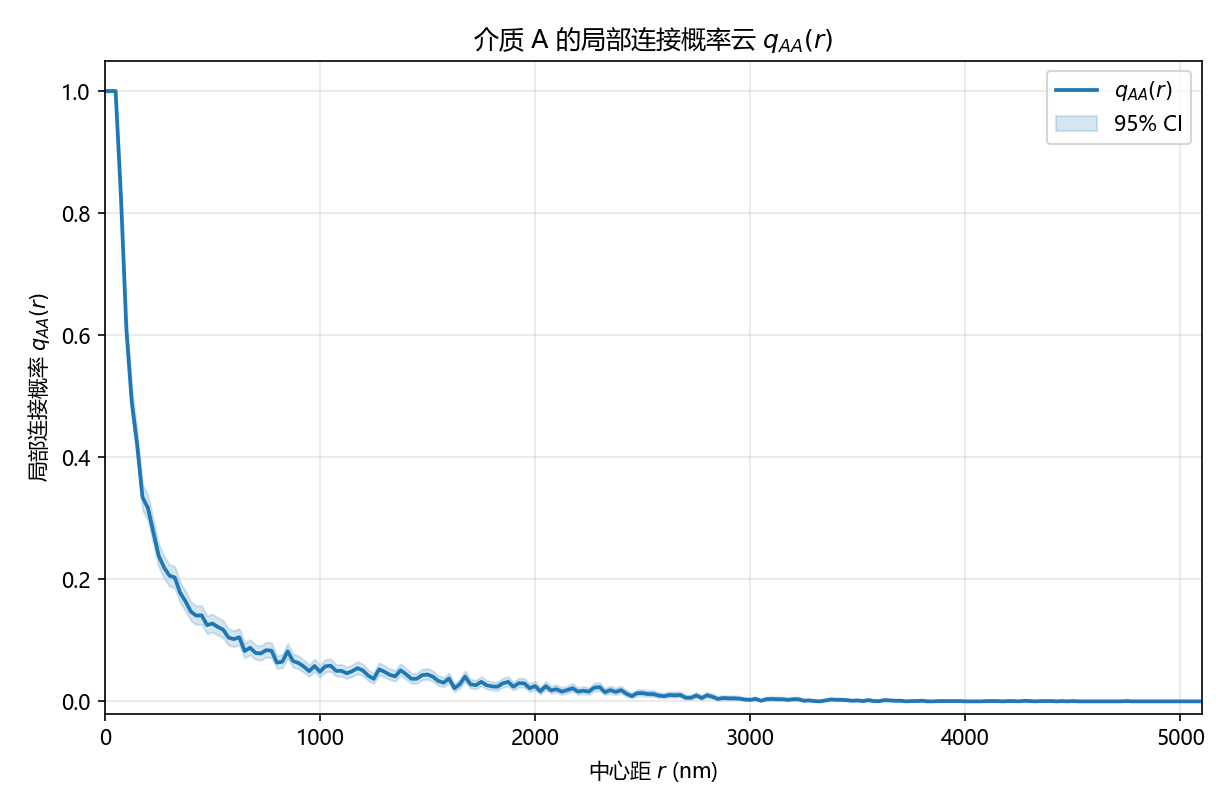
\includegraphics[width=0.75\textwidth]{version_log/2.0.0/conductive_microstructure/results/figures/problem2_q_aa.png}
    \caption{介质 A 的局部连接概率云 $q_{AA}(r)$。当中心距较小时两根圆柱几乎必连接，随着中心距增加，连接概率快速下降并形成长尾。}
    \label{fig:q2_qaa}
\end{figure}

\begin{figure}[htbp]
    \centering
    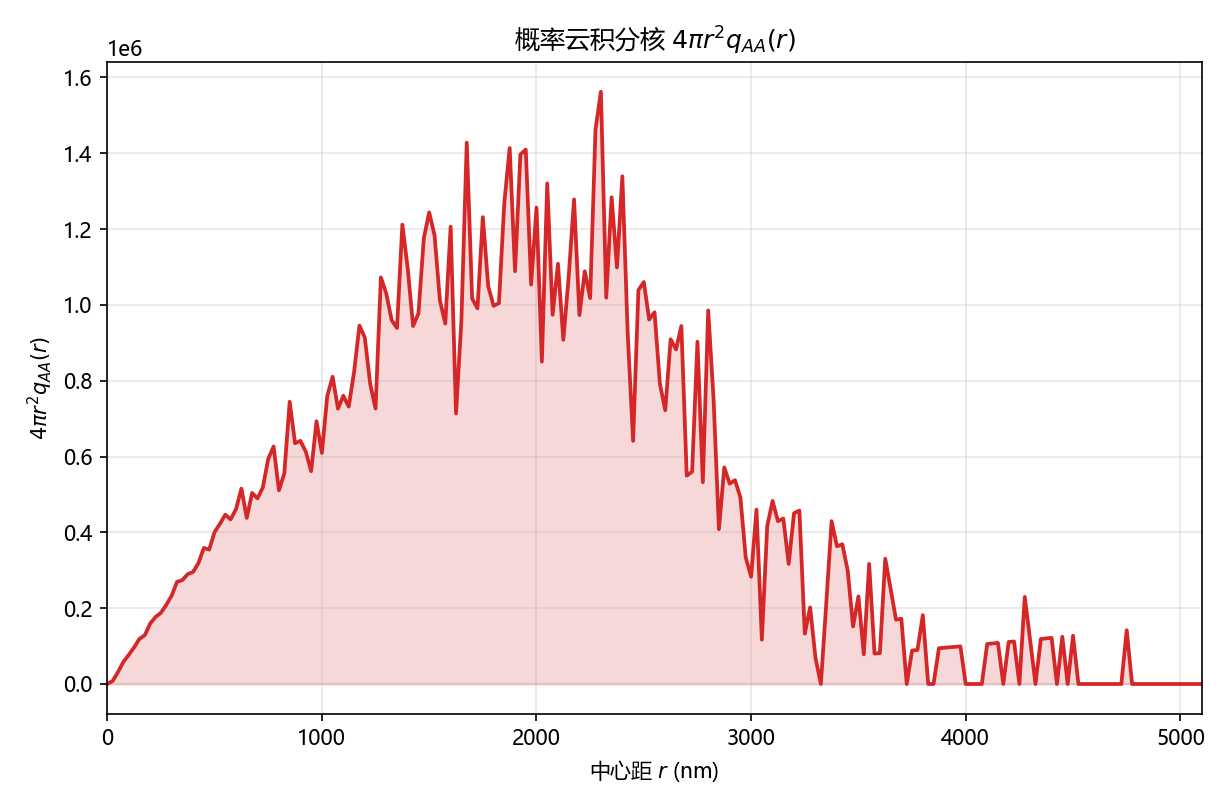
\includegraphics[width=0.75\textwidth]{version_log/2.0.0/conductive_microstructure/results/figures/problem2_4pir2q.png}
    \caption{概率云积分核 $4\pi r^2 q_{AA}(r)$。该曲线对 $r$ 的积分即为等效连接体积 $V_{AA}$。}
    \label{fig:q2_4pir2q}
\end{figure}

\subsection{Monte Carlo 贯通概率仿真}

对每组参数 $(\phi,\text{boundary mode})$，随机生成 $N_A$ 根圆柱并在边界回绕后切分为在箱片段；随后利用 AABB 宽相位筛选候选片段对，结合精确判距建立随机几何图，再判断左右电极是否连通。重复多次试验后，以
\[
\hat{P}_{\mathrm{conn}}=\frac{\text{贯通次数}}{\text{试验总次数}}
\]
估计导通概率，并给出 Wilson $95\%$ 置信区间。

\subsection{问题 2 结果与理论验证}

在 $\phi\in\{0.50\%,0.60\%,0.70\%,1.00\%\}$ 下得到的结果如表 \ref{tab:q2_result} 所示。

\begin{table}[htbp]
    \centering
    \caption{问题 2 在不同体积分数下的导通概率结果}
    \label{tab:q2_result}
    \begin{tabular}{ccccc}
        \hline
        $\phi(\%)$ & $N_A$ & 周期连续 $\hat{P}_{\mathrm{conn}}$ & 仅几何回绕 $\hat{P}_{\mathrm{conn}}$ & $\bar{k}$ \\
        \hline
        0.50 & 354 & 0.9150 & 0.9180 & 0.902 \\
        0.60 & 424 & 0.9505 & 0.9575 & 1.081 \\
        0.70 & 495 & 0.9750 & 0.9765 & 1.262 \\
        1.00 & 707 & 0.9965 & 0.9970 & 1.802 \\
        \hline
    \end{tabular}
\end{table}

结果显示：随着体积分数增加，系统导通概率单调上升；两种边界模式下的差异均小于 $0.7\%$，说明对于随机填充体系，边界解释对总体结论影响较小。更重要的是，当 $\bar{k}$ 从 $0.90$ 增加到 $1.08$ 时，导通概率恰好由“刚过 $90\%$ 阈值”跃升至接近 $95\%$。这说明：
\begin{quote}
    概率云给出的平均连接度 $\bar{k}$ 能有效刻画局部连接能力，并能正确预测宏观导通从临界区向高概率贯通区的转变趋势。
\end{quote}
与此同时，最大连通分量占比 $S_{\max}/N$ 也随体积分数单调升高：在 $\phi=0.50\%$ 时，两种边界模式下已分别达到 $0.9057$ 与 $0.9333$；到 $\phi=1.00\%$ 时则上升至 $0.9829$ 与 $0.9888$。这说明在临界区附近，网络并不是由大量彼此分离的小团簇组成，而是已经形成占主导地位的连通骨架。

因此，问题 2 为后续问题 3 和问题 4 提供了坚实的理论基础：概率云模型不仅可以解释仿真结果，而且可以作为后续优化搜索的理论先导。

\begin{figure}[htbp]
    \centering
    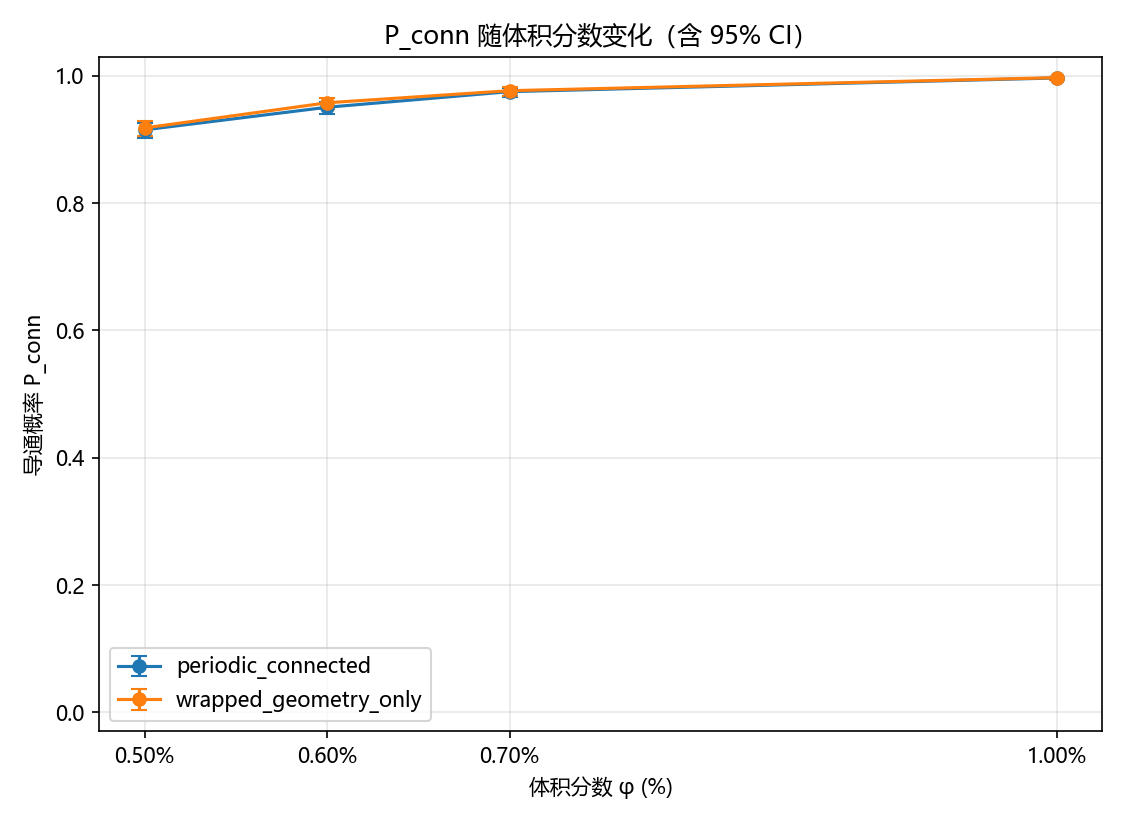
\includegraphics[width=0.72\textwidth]{version_log/2.0.0/conductive_microstructure/results/figures/problem2_p_conn.png}
    \caption{问题 2 中导通概率 $P_{\mathrm{conn}}$ 随体积分数 $\phi$ 的变化，两种边界模式下结果均随 $\phi$ 增大而单调上升。}
    \label{fig:q2_pconn}
\end{figure}

\begin{figure}[htbp]
    \centering
    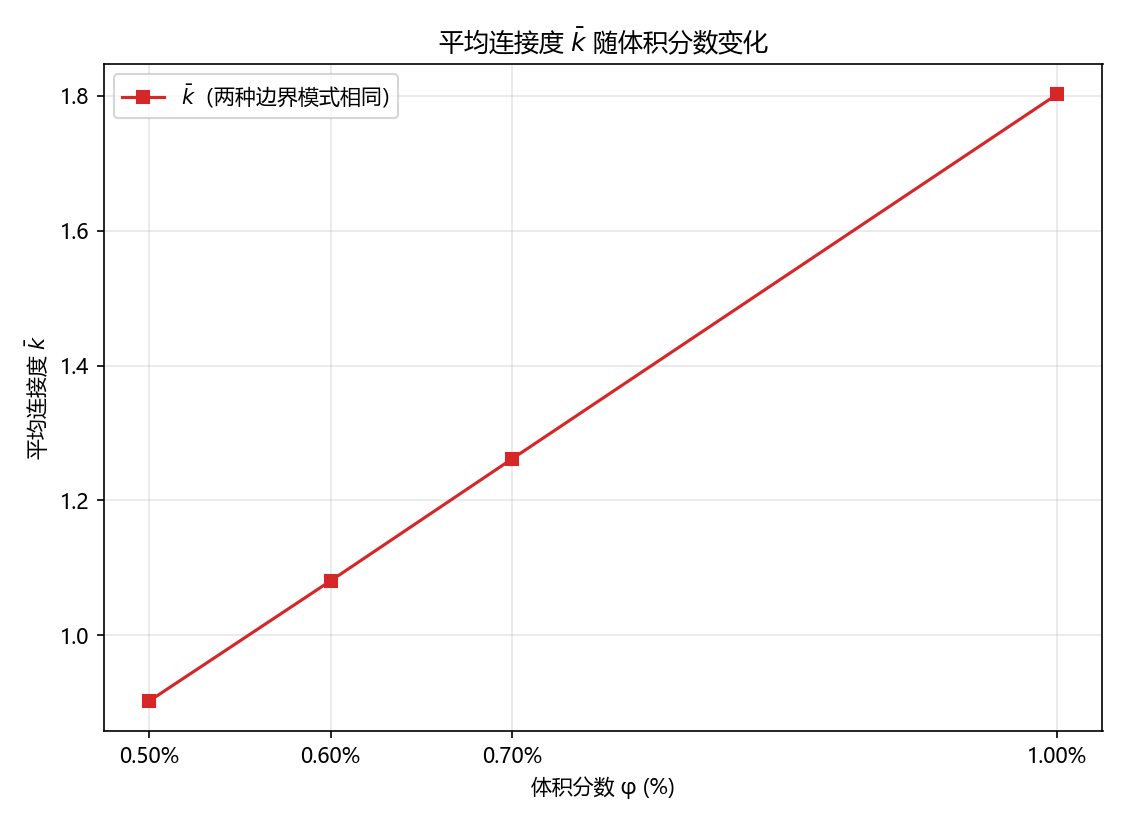
\includegraphics[width=0.72\textwidth]{version_log/2.0.0/conductive_microstructure/results/figures/problem2_kbar.png}
    \caption{问题 2 中概率云理论平均连接度 $\bar{k}$ 随体积分数 $\phi$ 的变化。随着填充率增加，单个节点的平均连接能力随之增强。}
    \label{fig:q2_kbar}
\end{figure}

\begin{figure}[htbp]
    \centering
    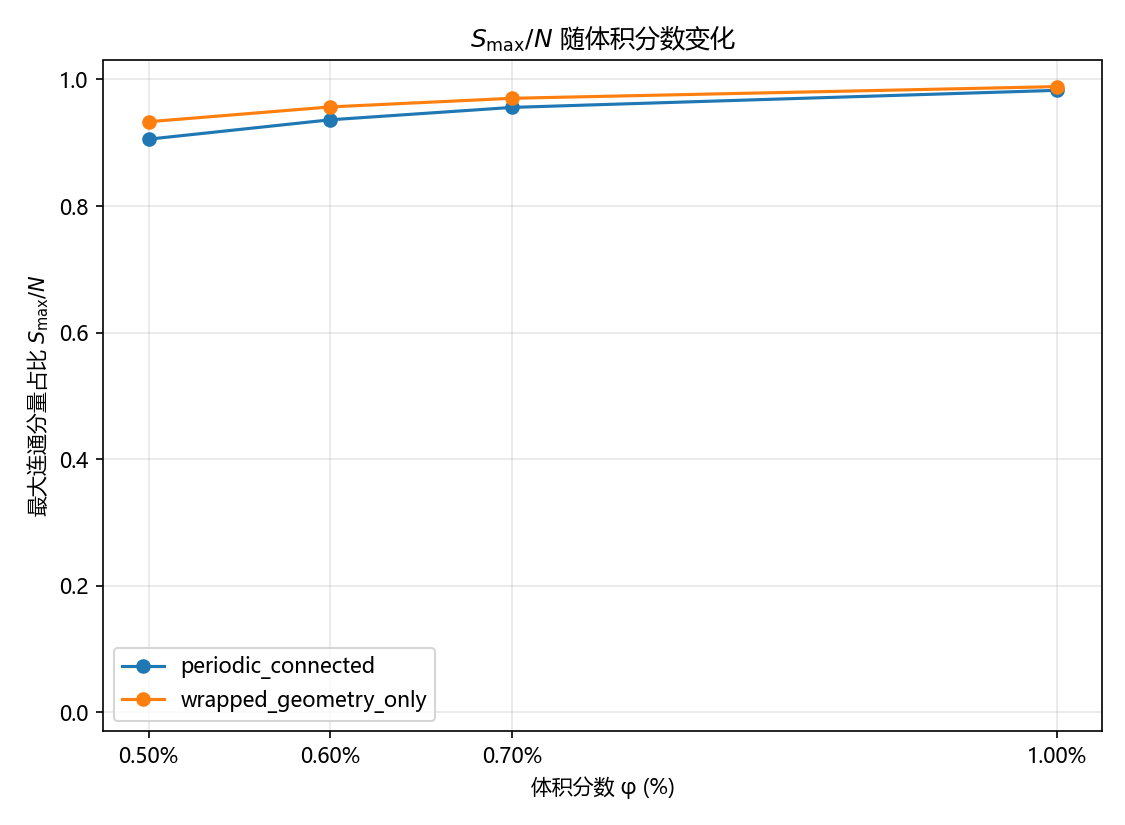
\includegraphics[width=0.72\textwidth]{version_log/2.0.0/conductive_microstructure/results/figures/problem2_smax_ratio.png}
    \caption{问题 2 中最大连通分量占比 $S_{\max}/N$ 随体积分数 $\phi$ 的变化。该指标反映了网络从分散小团簇向主导连通骨架演化的过程。}
    \label{fig:q2_smax}
\end{figure}

\begin{figure}[htbp]
    \centering
    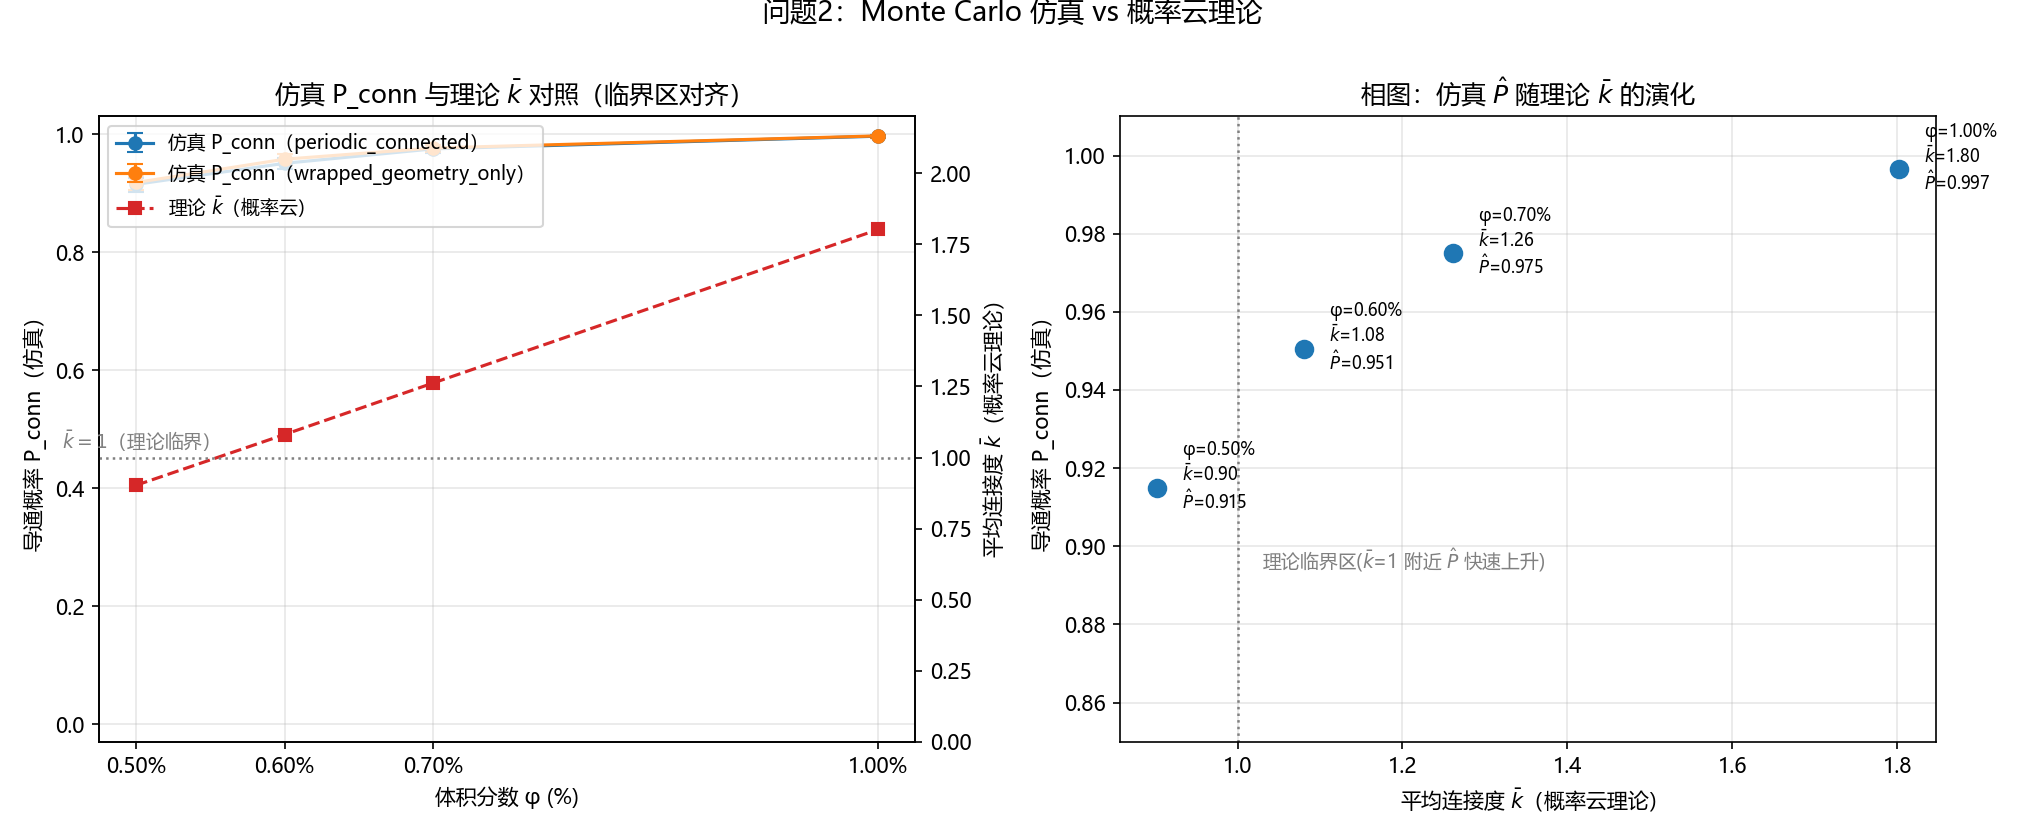
\includegraphics[width=0.92\textwidth]{version_log/2.0.0/conductive_microstructure/results/figures/problem2_theory_vs_simulation.png}
    \caption{问题 2 中 Monte Carlo 仿真与概率云理论的对照。左图展示导通概率与平均连接度随体积分数的变化，右图给出 $\hat{P}_{\mathrm{conn}}$ 与 $\bar{k}$ 的对应关系。}
    \label{fig:q2_theory_vs_sim}
\end{figure}

\section{问题 3：满足 \texorpdfstring{$P_{\mathrm{conn}}\ge 90\%$}{Pconn>=90\%} 的最低填充率}

\subsection{二分搜索与单侧置信判据}

问题 3 的目标是求满足
\[
P_{\mathrm{conn}}\ge 0.90
\]
时介质 A 的最低体积分数 $\phi_{\min}$。由于填充率越大，体系整体连边越多，贯通概率总体上单调不减，因此可在区间
\[
[\phi_{\mathrm{low}},\phi_{\mathrm{high}}]=[0.20\%,0.70\%]
\]
上采用二分搜索。

为了避免仅凭点估计作出过于乐观的判断，本文使用 Wilson 单侧 $95\%$ 置信下界
\[
p_{\mathrm{lower},95\%}\ge 0.90
\]
作为“达标”的统计判据。若直接使用 $\hat{P}_{\mathrm{conn}}\ge 0.90$，则在真实概率恰处于临界附近时，容易因抽样波动而误判；而采用单侧置信下界可以保证结论更稳健。

\subsection{理论临界值}

由问题 2 已得
\[
V_{AA}=2.5493\times 10^9\,\mathrm{nm}^3.
\]
令平均连接度满足
\[
\bar{k}=1,
\]
即可得到理论临界填充率
\[
\phi_{\mathrm{theory}}=\frac{V_A}{V_{AA}}\approx 0.005546=0.5546\%.
\]
这并不是“$90\%$ 导通”的精确解析公式，而是一个用于描述渗流临界位置的理论参考值。

\subsection{问题 3 结果}

在二分中点使用 $1000$ 次试验判定，收敛后对候选点使用 $4000$ 次试验复核，得到表 \ref{tab:q3_result}。

\begin{table}[htbp]
    \centering
    \caption{问题 3 的最低填充率结果}
    \label{tab:q3_result}
    \begin{tabular}{cccccc}
        \hline
        边界模式 & $\phi_{\min}$ & $N_A$ & $\hat{P}_{\mathrm{conn}}$ & $p_{\mathrm{lower},95\%}$ & $\phi_{\mathrm{theory}}$ \\
        \hline
        周期连续 & 0.5125\% & 363 & 0.9155 & 0.9080 & 0.5546\% \\
        仅几何回绕 & 0.4969\% & 351 & 0.9075 & 0.8997 & 0.5546\% \\
        \hline
    \end{tabular}
\end{table}

可以看到，两种模式下的最低填充率都落在 $0.50\%$ 附近，且略低于理论临界值 $0.5546\%$。这表明概率云理论给出的临界参考与真实仿真结果在量级和变化方向上是一致的。其偏低的原因在于：介质 A 长径比较大，链式连接能力较强，因此在有限尺寸盒体中，达到 $90\%$ 贯通概率时所需的体积分数可以略低于均值场意义下的 $\bar{k}=1$ 临界点。

需要如实说明的是，\texttt{wrapped\_geometry\_only} 模式下最终 $4000$ 次复核得到
\[
p_{\mathrm{lower},95\%}=0.8997,
\]
略低于 $0.90$。这说明该点位于统计临界附近，属于由有限样本波动带来的边界现象，而不是模型失效。相较于问题 2 的趋势验证，问题 3 进一步给出了概率云理论与实际临界填充率之间的定量对应关系。

\begin{figure}[htbp]
    \centering
    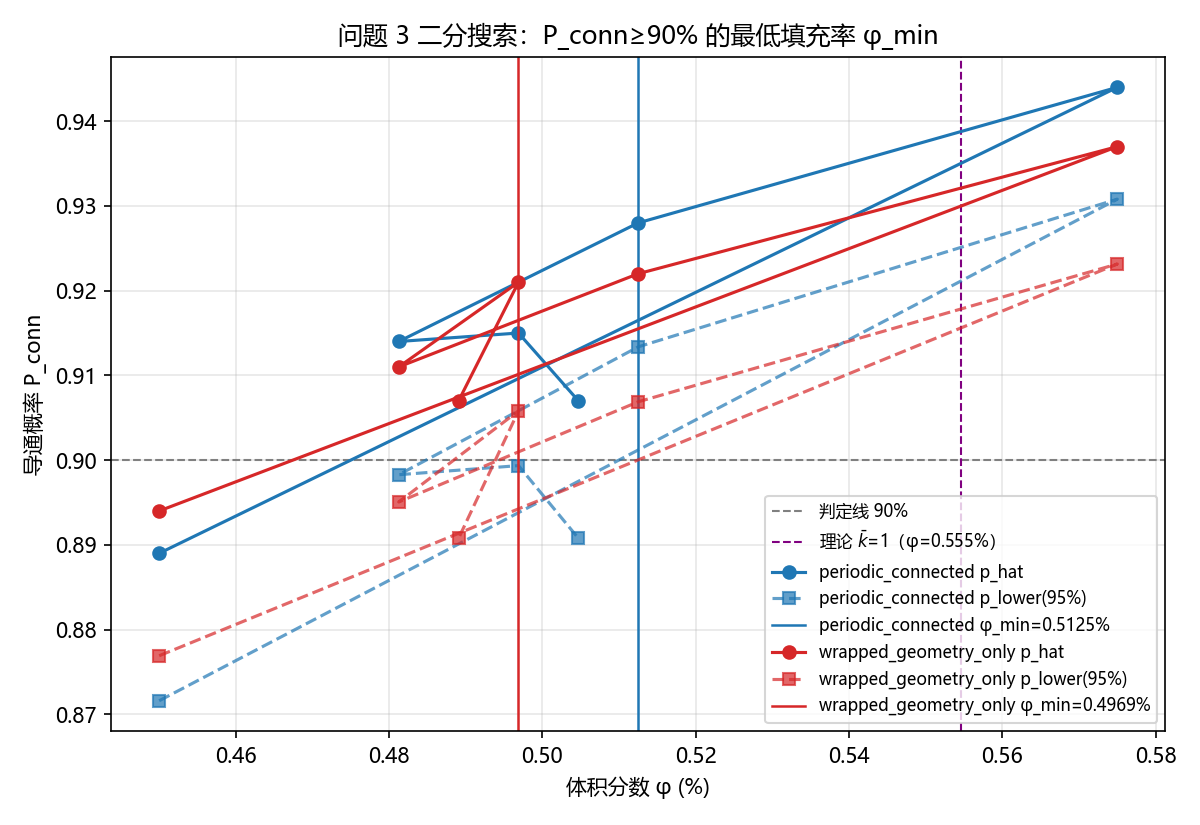
\includegraphics[width=0.72\textwidth]{version_log/2.0.0/conductive_microstructure/results/problem3/problem3_bisection.png}
    \caption{问题 3 中最低填充率的二分搜索过程示意图。图中展示了不同候选填充率下的判定结果及最终收敛区间。}
    \label{fig:q3_bisection}
\end{figure}

\section{问题 4：A/B 混合体系的最低成本组合}

\subsection{A/B 混合导通判据与成本函数}

在问题 4 中，除介质 A 外引入介质 B。其球心均匀分布在
\[
[-4800,4800]^3
\]
内，以保证球体完全落在盒内。混合体系的导通判据为：
\[
d_{AA}\le 61.8\,\mathrm{nm},\qquad
d_{AB}\le 231.8\,\mathrm{nm},\qquad
d_{BB}\le 401.8\,\mathrm{nm},
\]
且 B 球与电极平面导通的条件为球面到平面距离不超过 $\delta$，对应球心到电极面的距离阈值为 $201.8\,\mathrm{nm}$。

总成本函数写为
\[
C(N_A,N_B)=1.05\cdot N_A\frac{V_A}{10^9}+0.05\cdot N_B\frac{V_B}{10^9},
\]
其中
\[
V_B=\frac{4}{3}\pi R_B^3\approx 3.351\times 10^7\,\mathrm{nm}^3.
\]
目标是在
\[
P_{\mathrm{conn}}\ge 0.90
\]
的约束下，使成本最小。

\subsection{双介质概率云与连接矩阵}

在问题 2 的概率云思想基础上，定义混合体系中的三种等效连接体积：
\[
V_{AA},\qquad V_{AB},\qquad V_{BB}.
\]
其中 $V_{AA}$ 由问题 2 已得；$V_{BB}$ 可解析计算为半径 $401.8\,\mathrm{nm}$ 球体的体积；$V_{AB}$ 通过采样 A 的方向与 B 相对位置方向后数值积分得到。本文计算结果为
\[
V_{AA}=2.5493\times 10^9\,\mathrm{nm}^3,
\]
\[
V_{AB}=9.0877\times 10^8\,\mathrm{nm}^3,
\]
\[
V_{BB}=2.7172\times 10^8\,\mathrm{nm}^3.
\]
进一步构造连接矩阵
\[
M=
\begin{bmatrix}
\rho_A V_{AA} & \rho_B V_{AB}\\
\rho_A V_{AB} & \rho_B V_{BB}
\end{bmatrix},
\]
并以其最大特征值 $\lambda_{\max}$ 作为理论可行区的筛选指标。

\subsection{三级搜索策略}

问题 4 的求解采用“理论筛选 + Monte Carlo 边界搜索 + 成本优化确认”的三级流程：
\begin{enumerate}
    \item 在 $(N_A,N_B)$ 网格上扫描 $\lambda_{\max}$，得到理论可行区；
    \item 对每个 $N_A$ 网格点，在 $N_B\in[0,5000]$ 上用整数二分搜索满足 $p_{\mathrm{lower},95\%}\ge 0.90$ 的最小 $N_B$，得到可行边界；
    \item 沿边界计算成本，选取最小成本候选，并在其邻域用 $4000$ 次试验复核，最终确定最优解。
\end{enumerate}
之所以采用这种流程，是因为纯粹二维暴力扫描计算量极大，而理论可行区能够显著缩小需要精细仿真的范围。

\subsection{问题 4 结果与经济解释}

最终得到的最优解如表 \ref{tab:q4_result} 所示。

\begin{table}[htbp]
    \centering
    \caption{问题 4 的最低成本组合结果}
    \label{tab:q4_result}
    \begin{tabular}{cccccc}
        \hline
        边界模式 & $N_A^\ast$ & $N_B^\ast$ & 最低成本/元 & $\hat{P}_{\mathrm{conn}}$ & $p_{\mathrm{lower},95\%}$ \\
        \hline
        周期连续 & 360 & 0  & 5.3438 & 0.9147 & 0.9072 \\
        仅几何回绕 & 340 & 50 & 5.1307 & 0.9095 & 0.9018 \\
        \hline
    \end{tabular}
\end{table}

与此同时，理论层给出的 $\lambda_{\max}\ge 1$ 可行区为
\[
N_A\in[0,360],\qquad N_B\in[400,5000].
\]
与 Monte Carlo 实际边界相比，理论可行区明显偏宽松，但两者在趋势上是一致的：随着 $N_A$ 增大，所需的 $N_B$ 总体下降。这说明连接矩阵仍然成功刻画了局部连接能力的变化方向，只是有限尺寸下的实际贯通要求比均值场阈值更严格。

从工程解释看，最重要的结论不是“B 球越多越好”，而是：
\begin{quote}
    最低成本方案始终以介质 A 为主，介质 B 仅在临界区起到少量桥接补强作用。
\end{quote}
这是因为 B 球虽然单位体积成本较低，但单颗粒体积较大、点接触导电效率不如细长圆柱高；因此若试图依靠大量 B 球单独建立贯通路径，成本反而更高。只有当 A 已经接近形成主骨架时，加入少量 B 球才具有明显的边际收益。

\begin{figure}[htbp]
    \centering
    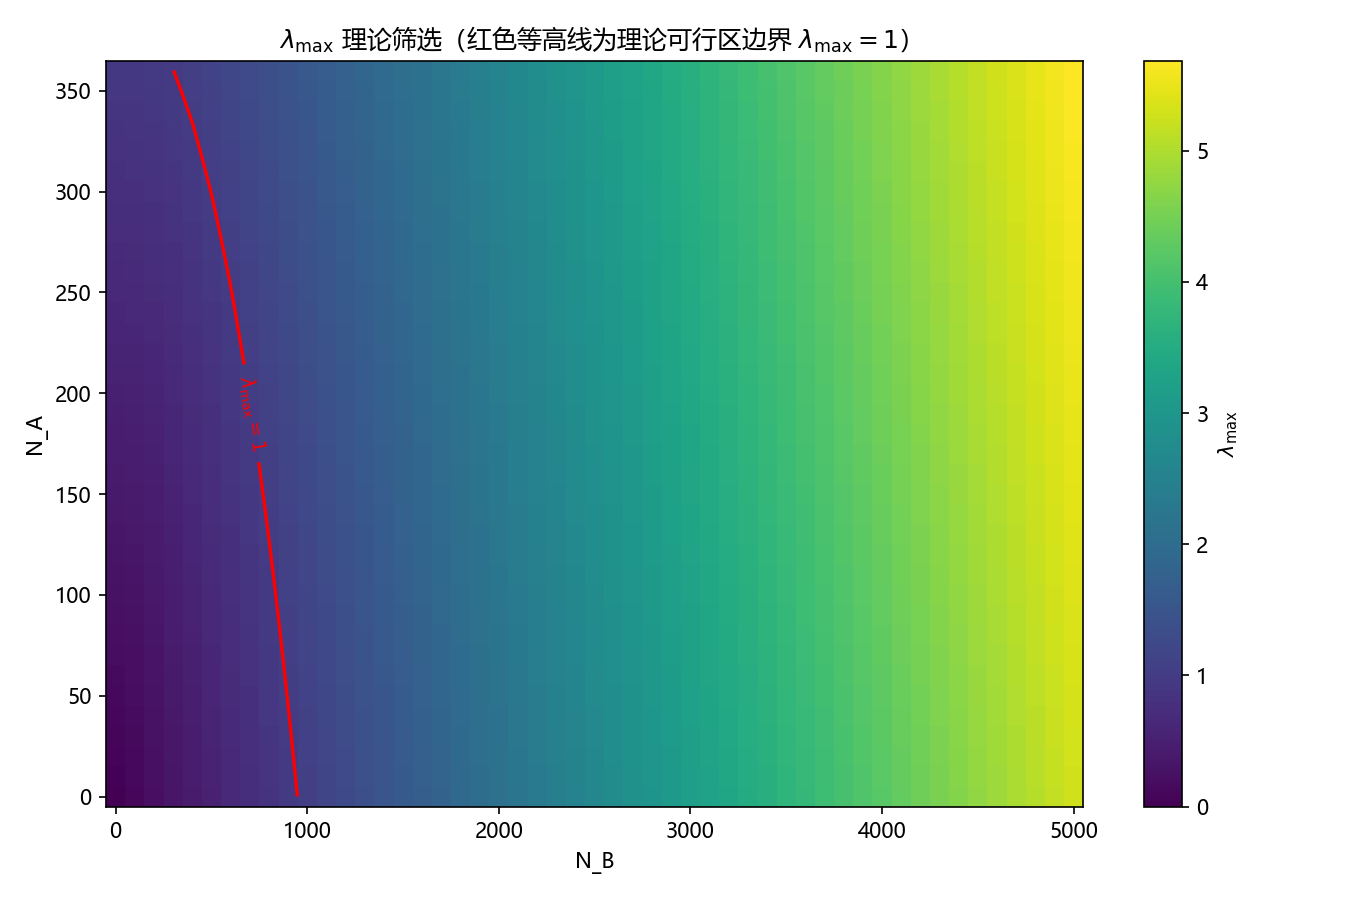
\includegraphics[width=0.78\textwidth]{version_log/2.0.0/conductive_microstructure/results/problem4/problem4_lambda_max_heatmap.png}
    \caption{问题 4 中 A/B 混合体系的 $\lambda_{\max}$ 理论热图。红色等高线对应 $\lambda_{\max}=1$，用于给出理论可行区。}
    \label{fig:q4_lambda}
\end{figure}

\begin{figure}[htbp]
    \centering
    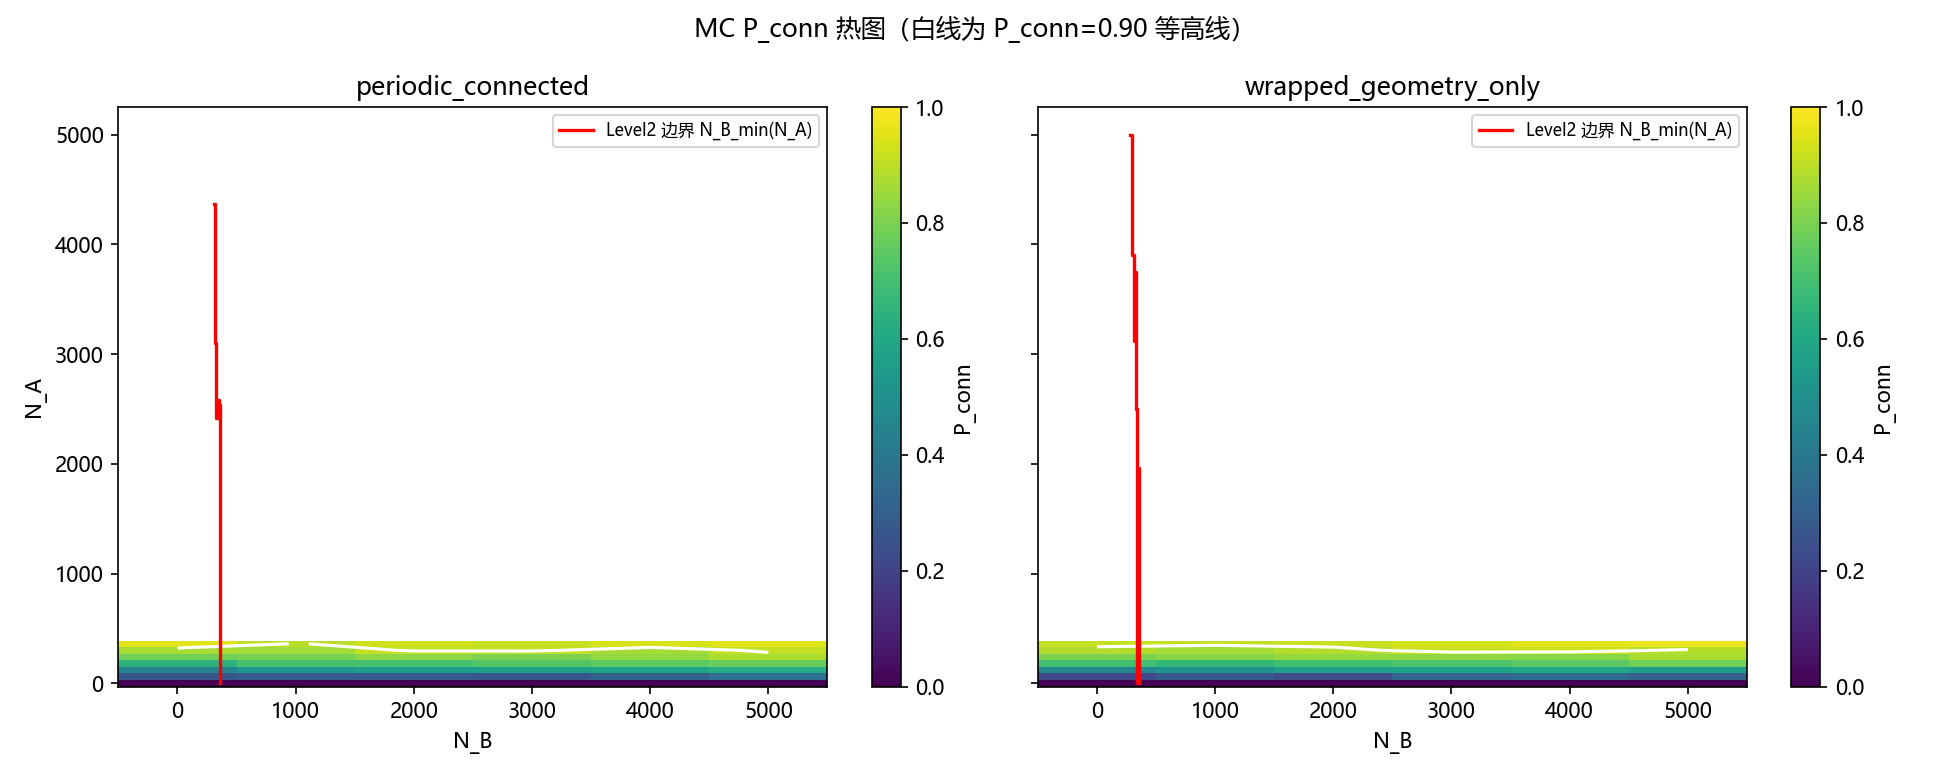
\includegraphics[width=0.92\textwidth]{version_log/2.0.0/conductive_microstructure/results/problem4/problem4_mc_pconn_heatmap.png}
    \caption{问题 4 中 A/B 混合体系的 Monte Carlo 导通概率热图。白色等高线为 $P_{\mathrm{conn}}=0.90$，红色阶梯线为二分搜索得到的可行边界。}
    \label{fig:q4_mc_heatmap}
\end{figure}

\begin{figure}[htbp]
    \centering
    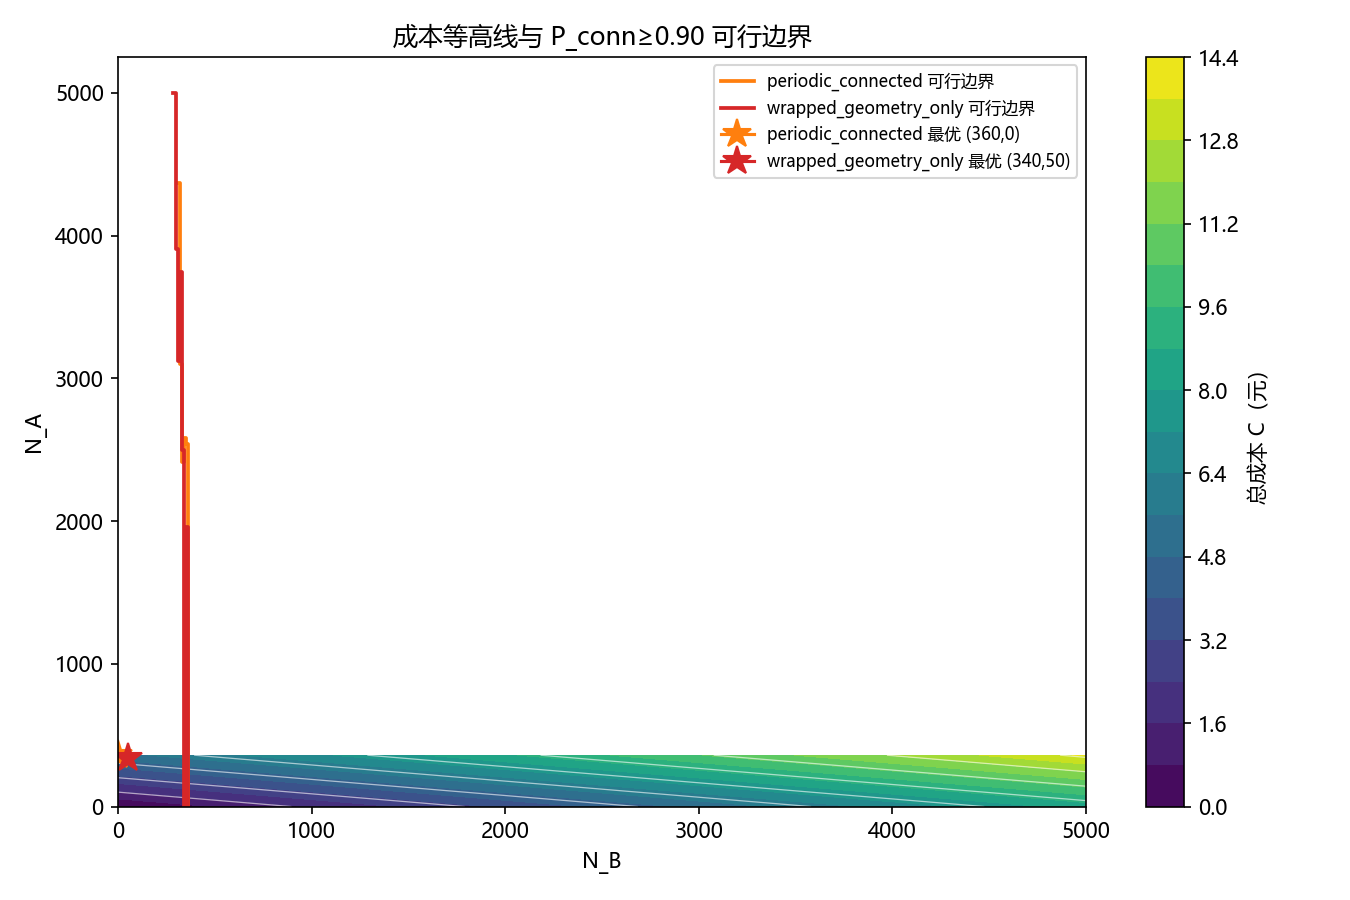
\includegraphics[width=0.78\textwidth]{version_log/2.0.0/conductive_microstructure/results/problem4/problem4_cost_boundary.png}
    \caption{问题 4 中成本等高线与可行边界。图中标出了满足 $P_{\mathrm{conn}}\ge 0.90$ 的最优组合位置。}
    \label{fig:q4_cost_boundary}
\end{figure}

\section{模型评价与结论}

\subsection{模型优点}

本文模型的主要优点体现在以下三个方面：
\begin{enumerate}
    \item 建立了统一的求解框架。问题 1 到问题 4 并非彼此割裂，而是围绕“局部连接 -- 宏观贯通 -- 优化决策”逐层展开；
    \item 理论与仿真互相支撑。概率云和连接矩阵负责解释渗流趋势与缩小搜索范围，Monte Carlo 负责给出有限尺寸盒体中的最终贯通概率；
    \item 结果具有较强可复现性。问题 3 的跨设备独立复现结果逐字节一致，说明当前随机种子派生和评估顺序设计可靠。
\end{enumerate}

\subsection{模型局限}

本文也存在以下局限：
\begin{enumerate}
    \item 圆柱之间的导通判据采用 capsule 近似，在端面附近存在微小几何误差；
    \item 概率云和连接矩阵基于各向同性随机分布的统计假设，未显式处理可能存在的取向偏置；
    \item 当前结论严格对应于题目给定的盒体尺度、几何参数和导通阈值，属于有限尺寸体系的工程结论。
\end{enumerate}

\subsection{全文结论}

综合问题 1 至问题 4 的结果，可以得到以下总体结论：
\begin{enumerate}
    \item 基于几何判距、边界处理和随机几何图的导通判定框架能够稳定刻画微构体中的导电贯通行为；
    \item 由局部连接概率云得到的等效连接体积与平均连接度，能够有效解释介质 A 体系中导通概率随填充率上升的规律；
    \item 满足 $P_{\mathrm{conn}}\ge 0.90$ 时，介质 A 的最低填充率约为 $0.50\%$，与理论临界值 $0.5546\%$ 同量级且方向一致，说明概率云理论已得到充分数值验证；
    \item 在 A/B 混合体系中，满足 $P_{\mathrm{conn}}\ge 0.90$ 的最低成本方案并不是以 B 为主体，而是以 A 为主、B 为辅的混合策略。
\end{enumerate}

因此，本文建立的“几何导通判据 -- 概率云 -- 渗流解释 -- Monte Carlo 验证 -- 优化求解”方法链，对微构体填充导电介质问题具有较好的统一解释能力和求解能力。

\section*{图表与结果文件对应说明}

正文涉及的主要图表可与现有结果文件对应如下。

公共目录：\texttt{version\_log/2.0.0/conductive\_microstructure/results/}

具体文件清单：
\begin{itemize}
    \small
    \item 问题 2 概率云图：\texttt{figures/problem2\_q\_aa.png}
    \item 问题 2 概率云积分核图：\texttt{figures/problem2\_4pir2q.png}
    \item 问题 2 导通概率图：\texttt{figures/problem2\_p\_conn.png}
    \item 问题 2 平均连接度图：\texttt{figures/problem2\_kbar.png}
    \item 问题 2 最大连通分量占比图：\texttt{figures/problem2\_smax\_ratio.png}
    \item 问题 2 理论--仿真对照图：\texttt{figures/problem2\_theory\_vs\_simulation.png}
    \item 问题 3 二分结果图：\texttt{problem3/problem3\_bisection.png}
    \item 问题 4 理论热图：\texttt{problem4/problem4\_lambda\_max\_heatmap.png}
    \item 问题 4 Monte Carlo 热图：\texttt{problem4/problem4\_mc\_pconn\_heatmap.png}
    \item 问题 4 成本边界图：\texttt{problem4/problem4\_cost\_boundary.png}
\end{itemize}

\section*{参考文献}

\begin{thebibliography}{99}
    \bibitem{huashu2026} 2026 第七届“华数杯”大学生数学建模竞赛 A 题：微构体中填充导电介质的仿真优化.
    \bibitem{attachment} 竞赛附件：\texttt{附件.xlsx}.
    \bibitem{format} 2026 第七届华数杯数学建模竞赛论文格式规范与提交说明.
\end{thebibliography}

% 说明：本文件从正文部分开始，不包含标题页、摘要页、关键词页、承诺页等第一页内容。

\section{问题重述与建模目标}

题目研究边长为 $10000\,\mathrm{nm}$ 的立方体微构体中导电介质随机填充后的贯通行为。微构体区域记为
\[
\Omega=[-5000,5000]^3,\qquad V_0=10^{12}\,\mathrm{nm}^3.
\]
体系中包含两类导电介质：
\begin{itemize}
    \item 介质 A：直圆柱，长度 $L_A=5000\,\mathrm{nm}$，半径 $R_A=30\,\mathrm{nm}$；
    \item 介质 B：球体，半径 $R_B=200\,\mathrm{nm}$。
\end{itemize}
左右带电面取为垂直于 $X$ 轴的两个平面
\[
x=-5000,\qquad x=5000.
\]
当两个导电介质之间，或导电介质与电极之间的最短距离满足
\[
d\le \delta,\qquad \delta=1.8\,\mathrm{nm}
\]
时，认为二者电学导通。若左右电极之间存在至少一条由导电介质组成的完整连接路径，则称微构体导通。

本题的四个问题可以统一归纳为：在既定几何规则和随机分布假设下，如何从局部导通判据出发，建立能够解释宏观贯通行为并完成参数优化的模型。围绕这一目标，本文建立如下统一技术路线：
\[
\boxed{
\begin{aligned}
\text{几何导通判据}
&\rightarrow
\text{局部连接概率云}
\rightarrow
\text{等效连接体积}\\
&\rightarrow
\text{随机几何图/连续渗流解释}
\rightarrow
\text{Monte Carlo 验证}\\
&\rightarrow
\text{临界填充率与成本优化}
\end{aligned}
}
\]
其中，问题 1 解决确定性结构的导通判定，问题 2 研究给定填充率时的导通概率，问题 3 求满足 $P_{\mathrm{conn}}\ge 0.90$ 时介质 A 的最低填充率，问题 4 在 $P_{\mathrm{conn}}\ge 0.90$ 的约束下求 A/B 混合体系的最低成本组合。

\section{模型假设}

为建立明确的概率测度并保持模型可计算，作如下假设：
\begin{enumerate}
    \item 所有介质位置独立均匀分布于微构体内；
    \item 介质 A 姿态服从球面各向同性分布；
    \item 介质之间允许重叠和贯穿，不考虑排斥体积效应；
    \item 不考虑重力、动态重排及时间演化，系统视为静态随机结构；
    \item 最短距离不超过 $1.8\,\mathrm{nm}$ 即视为理想导通；
    \item 同一导电介质内部视为整体等势导体；
    \item 除题目给出的边界截断/回绕规则外，不额外引入表面效应；
    \item Monte Carlo 各次试验彼此独立。
\end{enumerate}

需要指出的是，第 1、2 条是建立导通概率模型的核心统计假设。本文中的概率云与连接矩阵用于描述\textbf{局部连接能力及渗流趋势}，有限尺寸微构体中沿电极方向的实际贯通概率最终仍由 Monte Carlo 仿真确定。因此，本文不作如下过强结论：$\bar{k}>1$ 时系统一定导通，或 $\lambda_{\max}>1$ 等价于 $90\%$ 导通。

\section{问题 1：三组确定性结构的导通判定}

\subsection{附件数据解释与边界模式}

附件 \texttt{附件.xlsx} 给出三组介质 A 的端点坐标数据，每行包含一根圆柱轴线段的两个端点。对数据核对后发现，附件中的部分轴线段长度小于 $5000\,\mathrm{nm}$，且存在多行端点在周期回绕后完全重合、长度和恰好为 $5000\,\mathrm{nm}$ 的现象。这说明附件中的一行并不总是完整圆柱，而可能是\textbf{经过边界截断后的在箱片段}。

因此，对边界规则作两种解释并分别计算：
\begin{enumerate}
    \item \texttt{PERIODIC\_CONNECTED}：跨边界后仍视为同一根导体，周期回绕后重合的片段合并为同一节点；
    \item \texttt{WRAPPED\_GEOMETRY\_ONLY}：仅做几何回绕，每一行数据都视为独立节点，不承认跨边界电学连续。
\end{enumerate}
这种双模式处理既保留了题目描述下的物理解释，也便于后续做敏感性分析。

\subsection{几何导通判据与建图}

将圆柱体用 capsule 近似表示为“轴线段向外膨胀半径 $R_A$”得到的几何体，则两根介质 A 导通的条件为
\[
d_{\mathrm{seg}} \le 2R_A+\delta = 61.8\,\mathrm{nm},
\]
其中 $d_{\mathrm{seg}}$ 为两条轴线段最短距离。介质 A 与电极平面导通条件为
\[
d_{\mathrm{axis\mbox{-}plane}} \le R_A+\delta = 31.8\,\mathrm{nm}.
\]
在计算实现中，先根据边界模式构造节点，再依据圆柱--圆柱和圆柱--电极的导通判据建立无向图，最后通过并查集和多源 BFS 判断左右电极是否处于同一连通分量并提取一条贯通路径。

\subsection{问题 1 结果与解释}

三组数据的判定结果如表 \ref{tab:q1_result} 所示。

\begin{table}[htbp]
    \centering
    \caption{问题 1 三组结构的导通判定结果}
    \label{tab:q1_result}
    \begin{tabular}{cccc}
        \hline
        分组 & 数据行数 & \texttt{PERIODIC\_CONNECTED} & \texttt{WRAPPED\_GEOMETRY\_ONLY} \\
        \hline
        组1 & 12  & 导通 & 不导通 \\
        组2 & 49  & 导通 & 导通 \\
        组3 & 535 & 导通 & 导通 \\
        \hline
    \end{tabular}
\end{table}

进一步统计表明，周期连续模式下组 1 的 12 行数据会被合并为 9 个节点，组 2 的 49 行会被合并为 39 个节点，组 3 的 535 行会被合并为 357 个节点。这说明附件数据中确实存在大量被边界截断后拆开的圆柱片段。

这一问的主要意义不在于三组结果本身，而在于为后续随机填充问题建立了一个可靠的几何基线：\textbf{边界处理方式、圆柱判距方法、建图与贯通判定框架已经得到验证}。其中，组 1 在两种边界解释下结论不同，恰好说明边界规则可能对个别确定性结构敏感；而组 2、组 3 在两种模式下均导通，说明其贯通性更为稳健。

\section{问题 2：给定填充率时的导通概率}

\subsection{随机生成模型}

对问题 2，仅考虑介质 A 的随机填充。设其体积分数为 $\phi$，则圆柱数目取为
\[
N_A=\mathrm{round}\!\left(\frac{\phi V_0}{V_A}\right),\qquad
V_A=\pi R_A^2L_A\approx 1.4137\times 10^7\,\mathrm{nm}^3.
\]
圆柱中心在盒内均匀分布，方向采用球面均匀采样。为避免极区聚集，不直接令极角 $\theta\sim U(0,\pi)$，而采用
\[
z=\cos\theta\sim U(-1,1),\qquad \varphi\sim U(0,2\pi),
\]
从而保证方向关于立体角均匀。

\subsection{局部连接概率云与等效连接体积}

固定两根介质 A 的中心距为 $r$，并令两根圆柱方向独立球面均匀，则定义径向连接概率云
\[
q_{AA}(r)=P(\text{两根 A 导通}\mid \text{中心距为 }r).
\]
对应的等效连接体积定义为
\[
V_{AA}=4\pi\int_0^\infty r^2 q_{AA}(r)\,\mathrm{d}r.
\]
本文通过 Monte Carlo 对 $q_{AA}(r)$ 逐点采样，再用数值积分得到
\[
V_{AA}=2.5493\times 10^9\,\mathrm{nm}^3.
\]
进一步定义平均连接度
\[
\bar{k}=\rho_A V_{AA},\qquad \rho_A=\frac{N_A}{V_0}.
\]
它反映了随机体系中单个节点的平均连接能力，可用于解释渗流临界附近的宏观行为变化。

\begin{figure}[htbp]
    \centering
    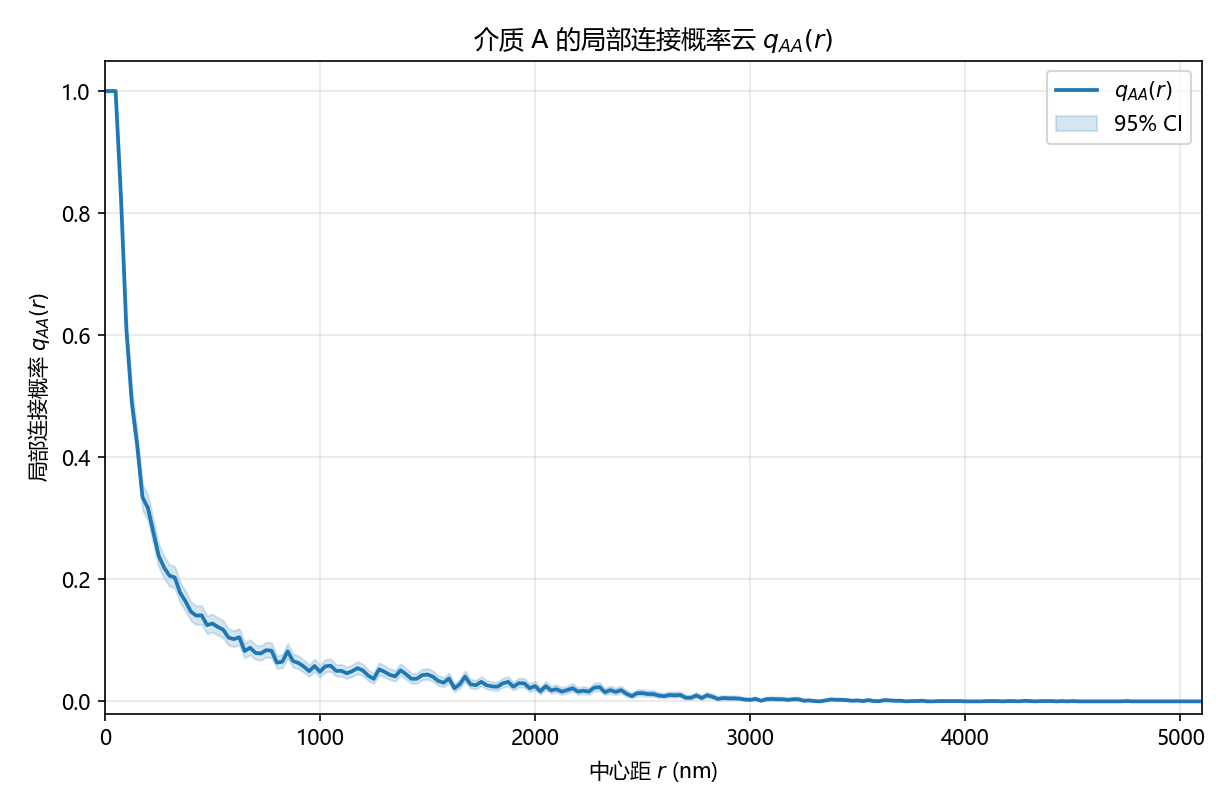
\includegraphics[width=0.75\textwidth]{version_log/2.0.0/conductive_microstructure/results/figures/problem2_q_aa.png}
    \caption{介质 A 的局部连接概率云 $q_{AA}(r)$。当中心距较小时两根圆柱几乎必连接，随着中心距增加，连接概率快速下降并形成长尾。}
    \label{fig:q2_qaa}
\end{figure}

\begin{figure}[htbp]
    \centering
    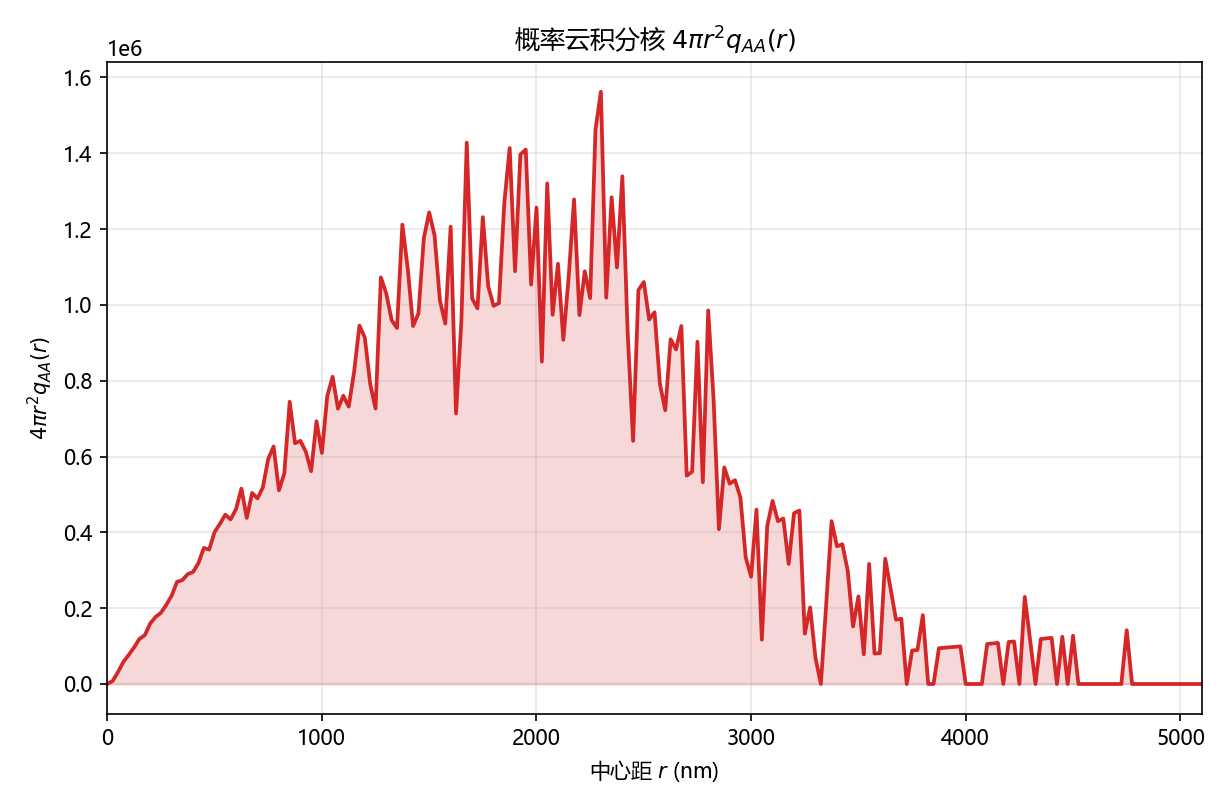
\includegraphics[width=0.75\textwidth]{version_log/2.0.0/conductive_microstructure/results/figures/problem2_4pir2q.png}
    \caption{概率云积分核 $4\pi r^2 q_{AA}(r)$。该曲线对 $r$ 的积分即为等效连接体积 $V_{AA}$。}
    \label{fig:q2_4pir2q}
\end{figure}

\subsection{Monte Carlo 贯通概率仿真}

对每组参数 $(\phi,\text{boundary mode})$，随机生成 $N_A$ 根圆柱并在边界回绕后切分为在箱片段；随后利用 AABB 宽相位筛选候选片段对，结合精确判距建立随机几何图，再判断左右电极是否连通。重复多次试验后，以
\[
\hat{P}_{\mathrm{conn}}=\frac{\text{贯通次数}}{\text{试验总次数}}
\]
估计导通概率，并给出 Wilson $95\%$ 置信区间。

\subsection{问题 2 结果与理论验证}

在 $\phi\in\{0.50\%,0.60\%,0.70\%,1.00\%\}$ 下得到的结果如表 \ref{tab:q2_result} 所示。

\begin{table}[htbp]
    \centering
    \caption{问题 2 在不同体积分数下的导通概率结果}
    \label{tab:q2_result}
    \begin{tabular}{ccccc}
        \hline
        $\phi(\%)$ & $N_A$ & 周期连续 $\hat{P}_{\mathrm{conn}}$ & 仅几何回绕 $\hat{P}_{\mathrm{conn}}$ & $\bar{k}$ \\
        \hline
        0.50 & 354 & 0.9150 & 0.9180 & 0.902 \\
        0.60 & 424 & 0.9505 & 0.9575 & 1.081 \\
        0.70 & 495 & 0.9750 & 0.9765 & 1.262 \\
        1.00 & 707 & 0.9965 & 0.9970 & 1.802 \\
        \hline
    \end{tabular}
\end{table}

结果显示：随着体积分数增加，系统导通概率单调上升；两种边界模式下的差异均小于 $0.7\%$，说明对于随机填充体系，边界解释对总体结论影响较小。更重要的是，当 $\bar{k}$ 从 $0.90$ 增加到 $1.08$ 时，导通概率恰好由“刚过 $90\%$ 阈值”跃升至接近 $95\%$。这说明：
\begin{quote}
    概率云给出的平均连接度 $\bar{k}$ 能有效刻画局部连接能力，并能正确预测宏观导通从临界区向高概率贯通区的转变趋势。
\end{quote}
与此同时，最大连通分量占比 $S_{\max}/N$ 也随体积分数单调升高：在 $\phi=0.50\%$ 时，两种边界模式下已分别达到 $0.9057$ 与 $0.9333$；到 $\phi=1.00\%$ 时则上升至 $0.9829$ 与 $0.9888$。这说明在临界区附近，网络并不是由大量彼此分离的小团簇组成，而是已经形成占主导地位的连通骨架。

因此，问题 2 为后续问题 3 和问题 4 提供了坚实的理论基础：概率云模型不仅可以解释仿真结果，而且可以作为后续优化搜索的理论先导。

\begin{figure}[htbp]
    \centering
    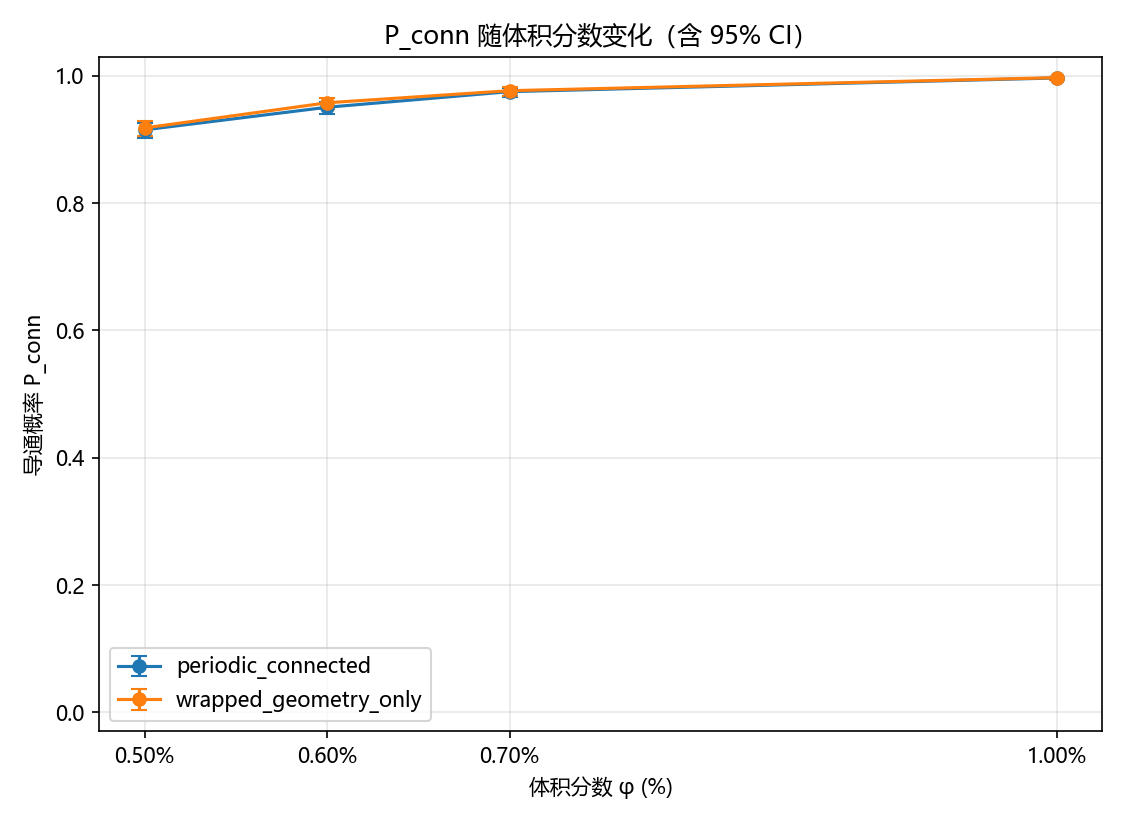
\includegraphics[width=0.72\textwidth]{version_log/2.0.0/conductive_microstructure/results/figures/problem2_p_conn.png}
    \caption{问题 2 中导通概率 $P_{\mathrm{conn}}$ 随体积分数 $\phi$ 的变化，两种边界模式下结果均随 $\phi$ 增大而单调上升。}
    \label{fig:q2_pconn}
\end{figure}

\begin{figure}[htbp]
    \centering
    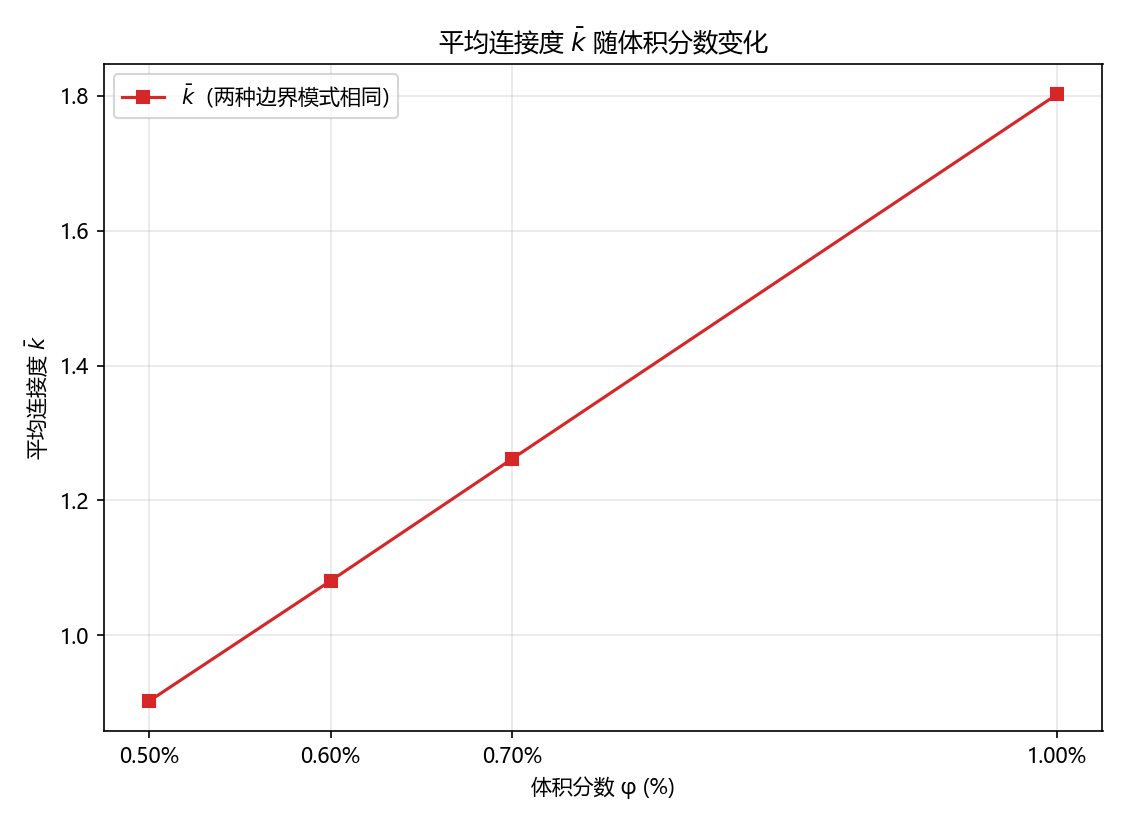
\includegraphics[width=0.72\textwidth]{version_log/2.0.0/conductive_microstructure/results/figures/problem2_kbar.png}
    \caption{问题 2 中概率云理论平均连接度 $\bar{k}$ 随体积分数 $\phi$ 的变化。随着填充率增加，单个节点的平均连接能力随之增强。}
    \label{fig:q2_kbar}
\end{figure}

\begin{figure}[htbp]
    \centering
    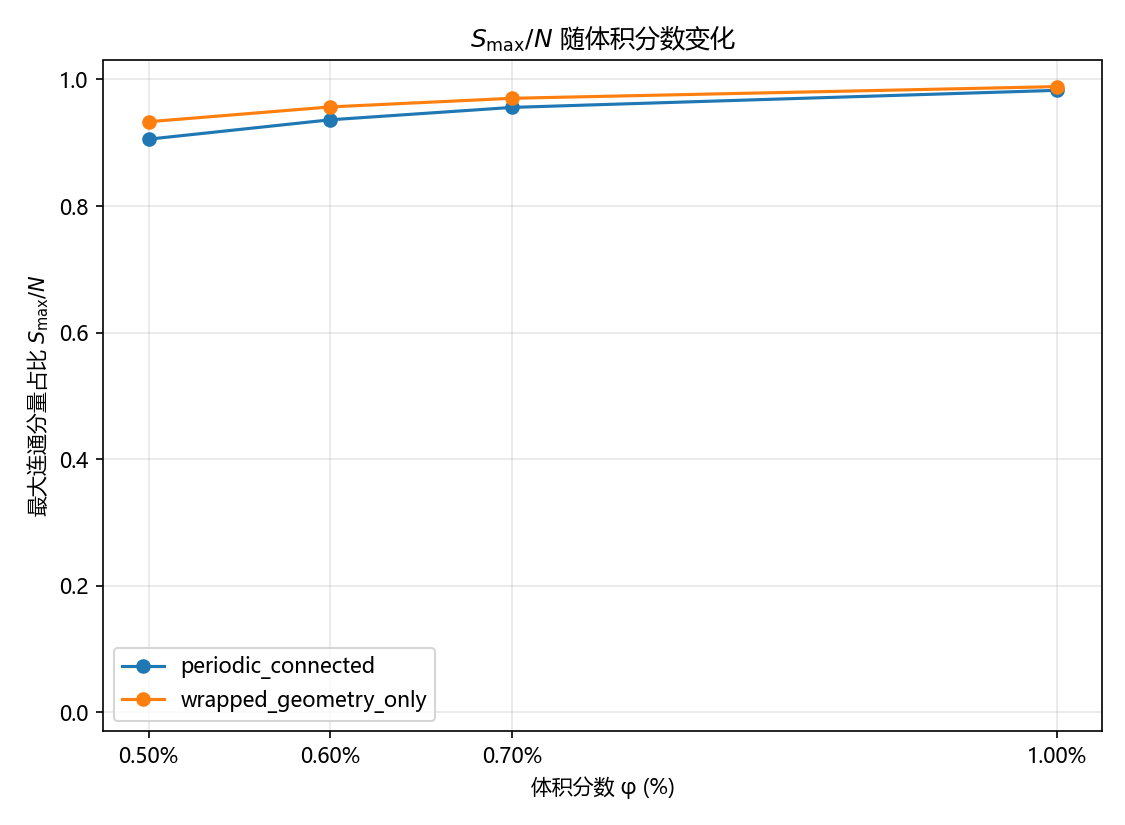
\includegraphics[width=0.72\textwidth]{version_log/2.0.0/conductive_microstructure/results/figures/problem2_smax_ratio.png}
    \caption{问题 2 中最大连通分量占比 $S_{\max}/N$ 随体积分数 $\phi$ 的变化。该指标反映了网络从分散小团簇向主导连通骨架演化的过程。}
    \label{fig:q2_smax}
\end{figure}

\begin{figure}[htbp]
    \centering
    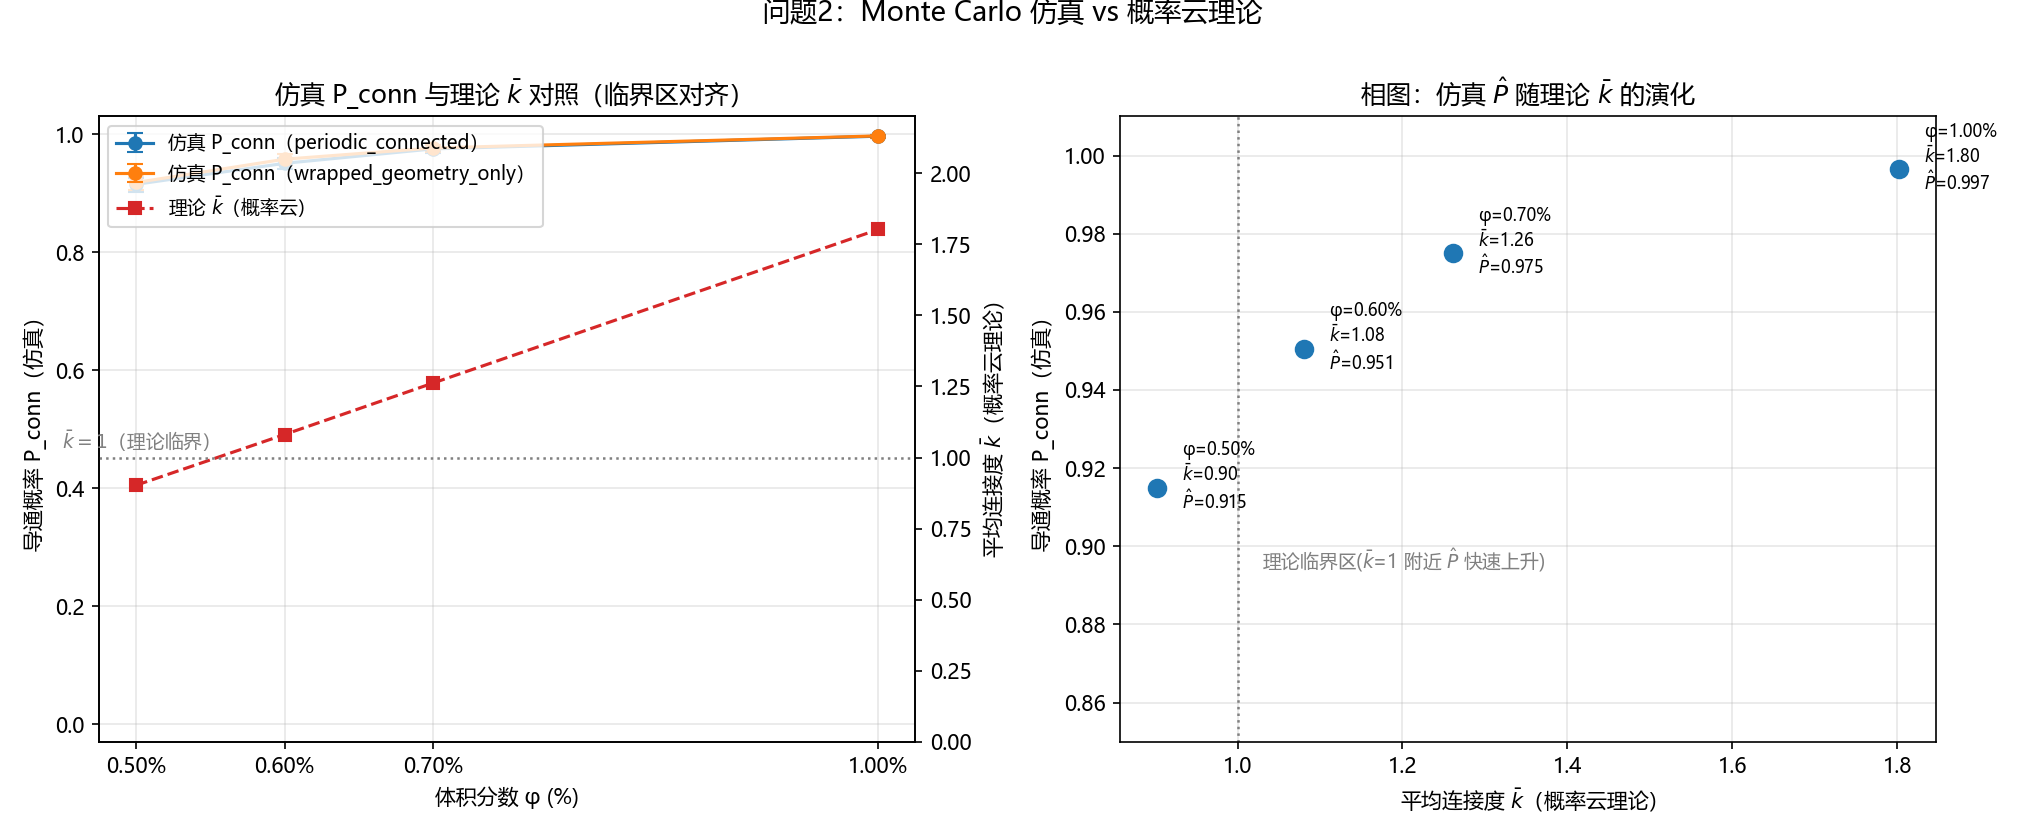
\includegraphics[width=0.92\textwidth]{version_log/2.0.0/conductive_microstructure/results/figures/problem2_theory_vs_simulation.png}
    \caption{问题 2 中 Monte Carlo 仿真与概率云理论的对照。左图展示导通概率与平均连接度随体积分数的变化，右图给出 $\hat{P}_{\mathrm{conn}}$ 与 $\bar{k}$ 的对应关系。}
    \label{fig:q2_theory_vs_sim}
\end{figure}

\section{问题 3：满足 \texorpdfstring{$P_{\mathrm{conn}}\ge 90\%$}{Pconn>=90\%} 的最低填充率}

\subsection{二分搜索与单侧置信判据}

问题 3 的目标是求满足
\[
P_{\mathrm{conn}}\ge 0.90
\]
时介质 A 的最低体积分数 $\phi_{\min}$。由于填充率越大，体系整体连边越多，贯通概率总体上单调不减，因此可在区间
\[
[\phi_{\mathrm{low}},\phi_{\mathrm{high}}]=[0.20\%,0.70\%]
\]
上采用二分搜索。

为了避免仅凭点估计作出过于乐观的判断，本文使用 Wilson 单侧 $95\%$ 置信下界
\[
p_{\mathrm{lower},95\%}\ge 0.90
\]
作为“达标”的统计判据。若直接使用 $\hat{P}_{\mathrm{conn}}\ge 0.90$，则在真实概率恰处于临界附近时，容易因抽样波动而误判；而采用单侧置信下界可以保证结论更稳健。

\subsection{理论临界值}

由问题 2 已得
\[
V_{AA}=2.5493\times 10^9\,\mathrm{nm}^3.
\]
令平均连接度满足
\[
\bar{k}=1,
\]
即可得到理论临界填充率
\[
\phi_{\mathrm{theory}}=\frac{V_A}{V_{AA}}\approx 0.005546=0.5546\%.
\]
这并不是“$90\%$ 导通”的精确解析公式，而是一个用于描述渗流临界位置的理论参考值。

\subsection{问题 3 结果}

在二分中点使用 $1000$ 次试验判定，收敛后对候选点使用 $4000$ 次试验复核，得到表 \ref{tab:q3_result}。

\begin{table}[htbp]
    \centering
    \caption{问题 3 的最低填充率结果}
    \label{tab:q3_result}
    \begin{tabular}{cccccc}
        \hline
        边界模式 & $\phi_{\min}$ & $N_A$ & $\hat{P}_{\mathrm{conn}}$ & $p_{\mathrm{lower},95\%}$ & $\phi_{\mathrm{theory}}$ \\
        \hline
        周期连续 & 0.5125\% & 363 & 0.9155 & 0.9080 & 0.5546\% \\
        仅几何回绕 & 0.4969\% & 351 & 0.9075 & 0.8997 & 0.5546\% \\
        \hline
    \end{tabular}
\end{table}

可以看到，两种模式下的最低填充率都落在 $0.50\%$ 附近，且略低于理论临界值 $0.5546\%$。这表明概率云理论给出的临界参考与真实仿真结果在量级和变化方向上是一致的。其偏低的原因在于：介质 A 长径比较大，链式连接能力较强，因此在有限尺寸盒体中，达到 $90\%$ 贯通概率时所需的体积分数可以略低于均值场意义下的 $\bar{k}=1$ 临界点。

需要如实说明的是，\texttt{wrapped\_geometry\_only} 模式下最终 $4000$ 次复核得到
\[
p_{\mathrm{lower},95\%}=0.8997,
\]
略低于 $0.90$。这说明该点位于统计临界附近，属于由有限样本波动带来的边界现象，而不是模型失效。相较于问题 2 的趋势验证，问题 3 进一步给出了概率云理论与实际临界填充率之间的定量对应关系。

\begin{figure}[htbp]
    \centering
    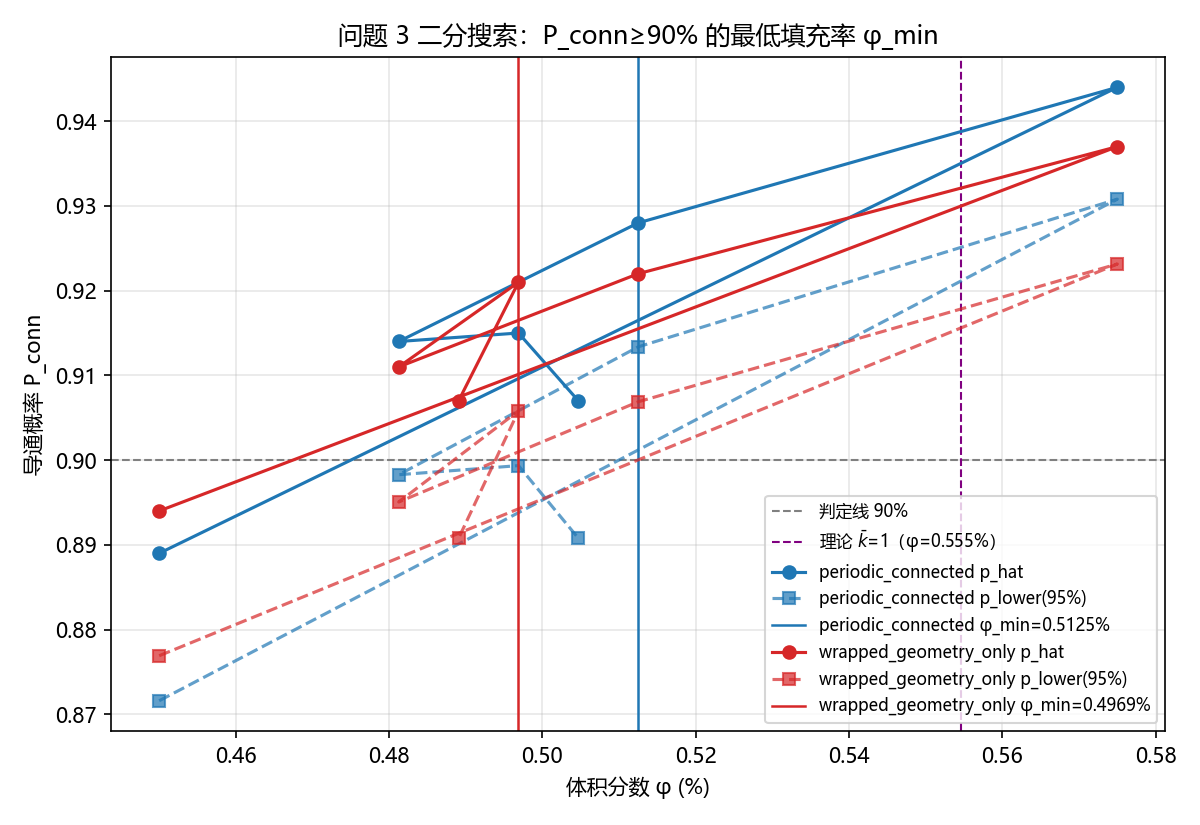
\includegraphics[width=0.72\textwidth]{version_log/2.0.0/conductive_microstructure/results/problem3/problem3_bisection.png}
    \caption{问题 3 中最低填充率的二分搜索过程示意图。图中展示了不同候选填充率下的判定结果及最终收敛区间。}
    \label{fig:q3_bisection}
\end{figure}

\section{问题 4：A/B 混合体系的最低成本组合}

\subsection{A/B 混合导通判据与成本函数}

在问题 4 中，除介质 A 外引入介质 B。其球心均匀分布在
\[
[-4800,4800]^3
\]
内，以保证球体完全落在盒内。混合体系的导通判据为：
\[
d_{AA}\le 61.8\,\mathrm{nm},\qquad
d_{AB}\le 231.8\,\mathrm{nm},\qquad
d_{BB}\le 401.8\,\mathrm{nm},
\]
且 B 球与电极平面导通的条件为球面到平面距离不超过 $\delta$，对应球心到电极面的距离阈值为 $201.8\,\mathrm{nm}$。

总成本函数写为
\[
C(N_A,N_B)=1.05\cdot N_A\frac{V_A}{10^9}+0.05\cdot N_B\frac{V_B}{10^9},
\]
其中
\[
V_B=\frac{4}{3}\pi R_B^3\approx 3.351\times 10^7\,\mathrm{nm}^3.
\]
目标是在
\[
P_{\mathrm{conn}}\ge 0.90
\]
的约束下，使成本最小。

\subsection{双介质概率云与连接矩阵}

在问题 2 的概率云思想基础上，定义混合体系中的三种等效连接体积：
\[
V_{AA},\qquad V_{AB},\qquad V_{BB}.
\]
其中 $V_{AA}$ 由问题 2 已得；$V_{BB}$ 可解析计算为半径 $401.8\,\mathrm{nm}$ 球体的体积；$V_{AB}$ 通过采样 A 的方向与 B 相对位置方向后数值积分得到。本文计算结果为
\[
V_{AA}=2.5493\times 10^9\,\mathrm{nm}^3,
\]
\[
V_{AB}=9.0877\times 10^8\,\mathrm{nm}^3,
\]
\[
V_{BB}=2.7172\times 10^8\,\mathrm{nm}^3.
\]
进一步构造连接矩阵
\[
M=
\begin{bmatrix}
\rho_A V_{AA} & \rho_B V_{AB}\\
\rho_A V_{AB} & \rho_B V_{BB}
\end{bmatrix},
\]
并以其最大特征值 $\lambda_{\max}$ 作为理论可行区的筛选指标。

\subsection{三级搜索策略}

问题 4 的求解采用“理论筛选 + Monte Carlo 边界搜索 + 成本优化确认”的三级流程：
\begin{enumerate}
    \item 在 $(N_A,N_B)$ 网格上扫描 $\lambda_{\max}$，得到理论可行区；
    \item 对每个 $N_A$ 网格点，在 $N_B\in[0,5000]$ 上用整数二分搜索满足 $p_{\mathrm{lower},95\%}\ge 0.90$ 的最小 $N_B$，得到可行边界；
    \item 沿边界计算成本，选取最小成本候选，并在其邻域用 $4000$ 次试验复核，最终确定最优解。
\end{enumerate}
之所以采用这种流程，是因为纯粹二维暴力扫描计算量极大，而理论可行区能够显著缩小需要精细仿真的范围。

\subsection{问题 4 结果与经济解释}

最终得到的最优解如表 \ref{tab:q4_result} 所示。

\begin{table}[htbp]
    \centering
    \caption{问题 4 的最低成本组合结果}
    \label{tab:q4_result}
    \begin{tabular}{cccccc}
        \hline
        边界模式 & $N_A^\ast$ & $N_B^\ast$ & 最低成本/元 & $\hat{P}_{\mathrm{conn}}$ & $p_{\mathrm{lower},95\%}$ \\
        \hline
        周期连续 & 360 & 0  & 5.3438 & 0.9147 & 0.9072 \\
        仅几何回绕 & 340 & 50 & 5.1307 & 0.9095 & 0.9018 \\
        \hline
    \end{tabular}
\end{table}

与此同时，理论层给出的 $\lambda_{\max}\ge 1$ 可行区为
\[
N_A\in[0,360],\qquad N_B\in[400,5000].
\]
与 Monte Carlo 实际边界相比，理论可行区明显偏宽松，但两者在趋势上是一致的：随着 $N_A$ 增大，所需的 $N_B$ 总体下降。这说明连接矩阵仍然成功刻画了局部连接能力的变化方向，只是有限尺寸下的实际贯通要求比均值场阈值更严格。

从工程解释看，最重要的结论不是“B 球越多越好”，而是：
\begin{quote}
    最低成本方案始终以介质 A 为主，介质 B 仅在临界区起到少量桥接补强作用。
\end{quote}
这是因为 B 球虽然单位体积成本较低，但单颗粒体积较大、点接触导电效率不如细长圆柱高；因此若试图依靠大量 B 球单独建立贯通路径，成本反而更高。只有当 A 已经接近形成主骨架时，加入少量 B 球才具有明显的边际收益。

\begin{figure}[htbp]
    \centering
    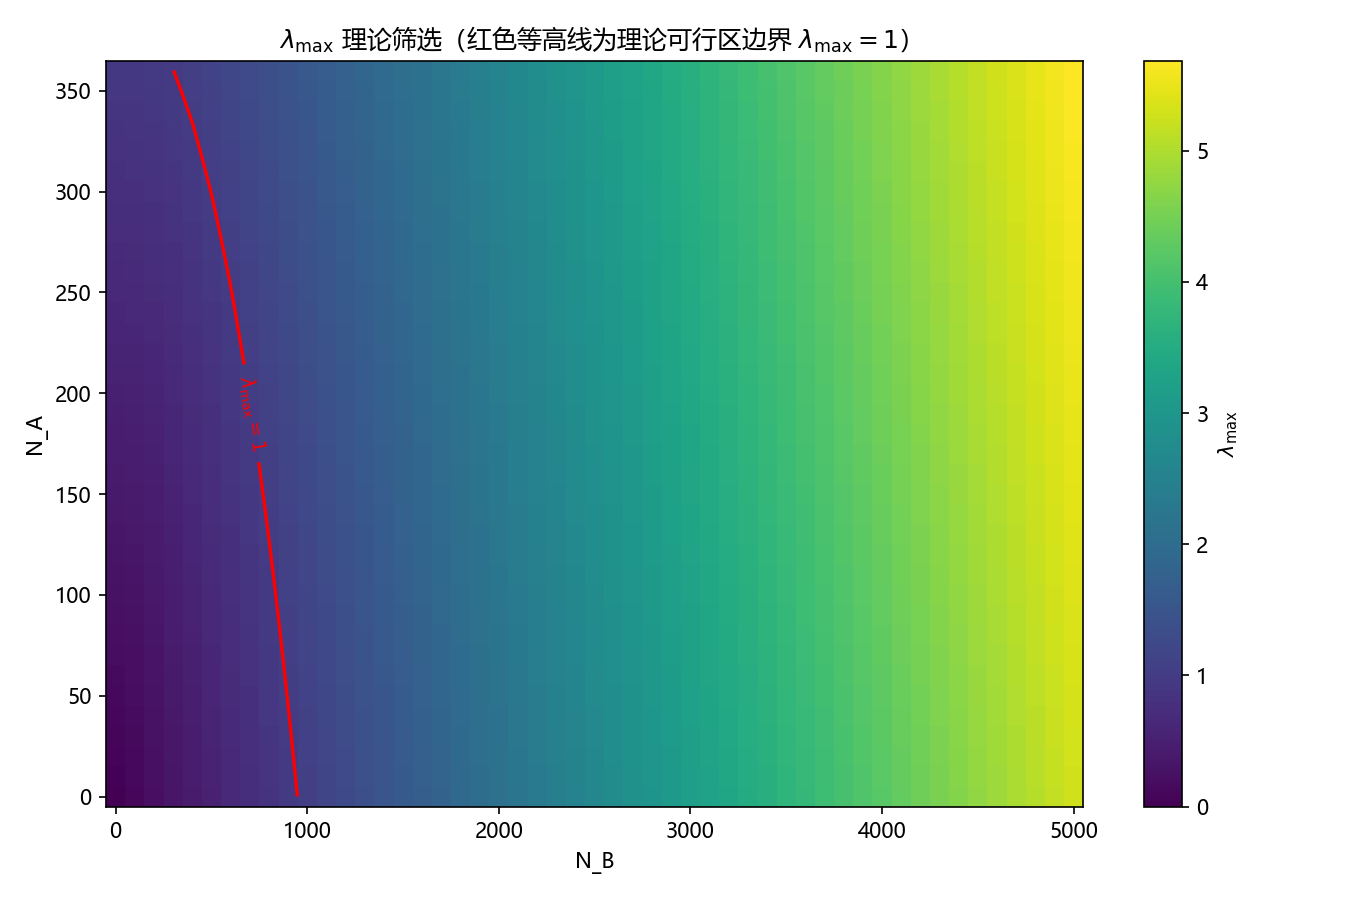
\includegraphics[width=0.78\textwidth]{version_log/2.0.0/conductive_microstructure/results/problem4/problem4_lambda_max_heatmap.png}
    \caption{问题 4 中 A/B 混合体系的 $\lambda_{\max}$ 理论热图。红色等高线对应 $\lambda_{\max}=1$，用于给出理论可行区。}
    \label{fig:q4_lambda}
\end{figure}

\begin{figure}[htbp]
    \centering
    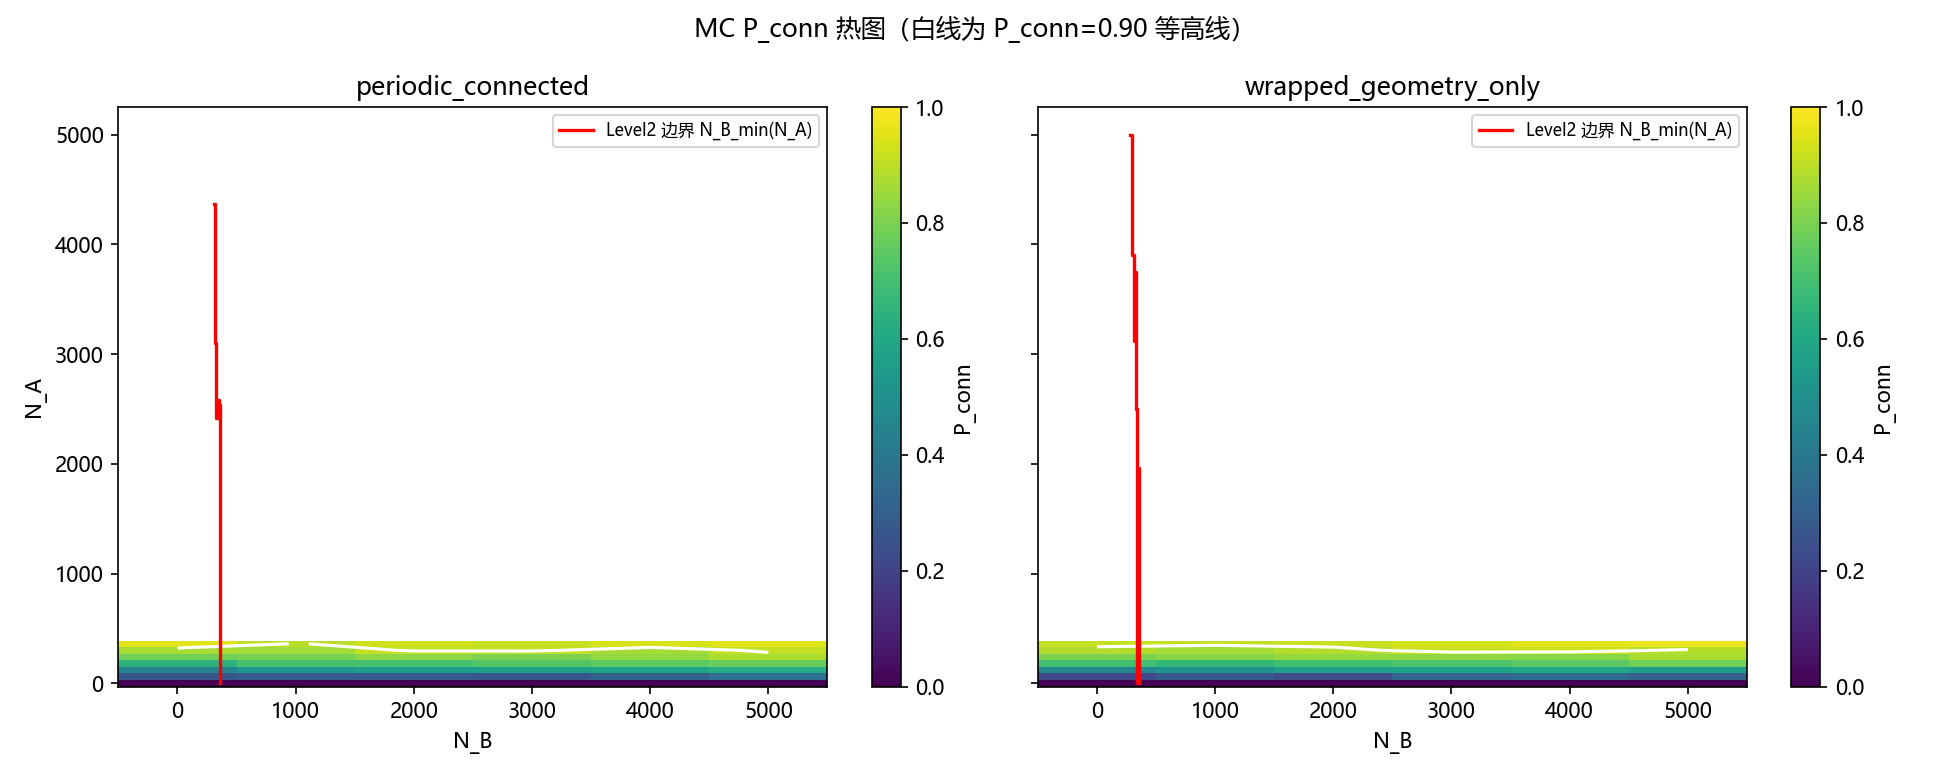
\includegraphics[width=0.92\textwidth]{version_log/2.0.0/conductive_microstructure/results/problem4/problem4_mc_pconn_heatmap.png}
    \caption{问题 4 中 A/B 混合体系的 Monte Carlo 导通概率热图。白色等高线为 $P_{\mathrm{conn}}=0.90$，红色阶梯线为二分搜索得到的可行边界。}
    \label{fig:q4_mc_heatmap}
\end{figure}

\begin{figure}[htbp]
    \centering
    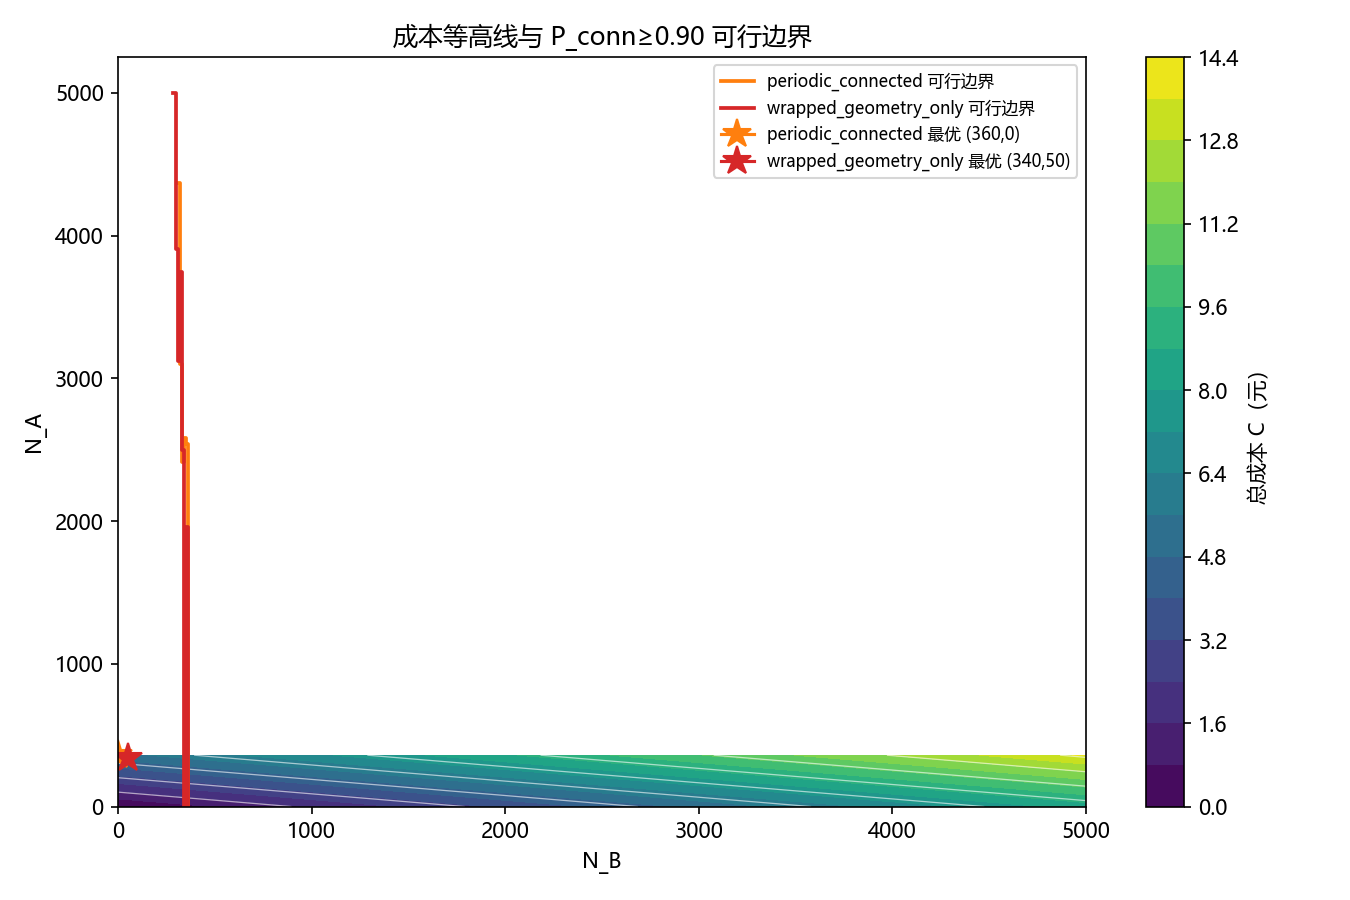
\includegraphics[width=0.78\textwidth]{version_log/2.0.0/conductive_microstructure/results/problem4/problem4_cost_boundary.png}
    \caption{问题 4 中成本等高线与可行边界。图中标出了满足 $P_{\mathrm{conn}}\ge 0.90$ 的最优组合位置。}
    \label{fig:q4_cost_boundary}
\end{figure}

\section{模型评价与结论}

\subsection{模型优点}

本文模型的主要优点体现在以下三个方面：
\begin{enumerate}
    \item 建立了统一的求解框架。问题 1 到问题 4 并非彼此割裂，而是围绕“局部连接 -- 宏观贯通 -- 优化决策”逐层展开；
    \item 理论与仿真互相支撑。概率云和连接矩阵负责解释渗流趋势与缩小搜索范围，Monte Carlo 负责给出有限尺寸盒体中的最终贯通概率；
    \item 结果具有较强可复现性。问题 3 的跨设备独立复现结果逐字节一致，说明当前随机种子派生和评估顺序设计可靠。
\end{enumerate}

\subsection{模型局限}

本文也存在以下局限：
\begin{enumerate}
    \item 圆柱之间的导通判据采用 capsule 近似，在端面附近存在微小几何误差；
    \item 概率云和连接矩阵基于各向同性随机分布的统计假设，未显式处理可能存在的取向偏置；
    \item 当前结论严格对应于题目给定的盒体尺度、几何参数和导通阈值，属于有限尺寸体系的工程结论。
\end{enumerate}

\subsection{全文结论}

综合问题 1 至问题 4 的结果，可以得到以下总体结论：
\begin{enumerate}
    \item 基于几何判距、边界处理和随机几何图的导通判定框架能够稳定刻画微构体中的导电贯通行为；
    \item 由局部连接概率云得到的等效连接体积与平均连接度，能够有效解释介质 A 体系中导通概率随填充率上升的规律；
    \item 满足 $P_{\mathrm{conn}}\ge 0.90$ 时，介质 A 的最低填充率约为 $0.50\%$，与理论临界值 $0.5546\%$ 同量级且方向一致，说明概率云理论已得到充分数值验证；
    \item 在 A/B 混合体系中，满足 $P_{\mathrm{conn}}\ge 0.90$ 的最低成本方案并不是以 B 为主体，而是以 A 为主、B 为辅的混合策略。
\end{enumerate}

因此，本文建立的“几何导通判据 -- 概率云 -- 渗流解释 -- Monte Carlo 验证 -- 优化求解”方法链，对微构体填充导电介质问题具有较好的统一解释能力和求解能力。

\section*{图表与结果文件对应说明}

正文涉及的主要图表可与现有结果文件对应如下。

公共目录：\texttt{version\_log/2.0.0/conductive\_microstructure/results/}

具体文件清单：
\begin{itemize}
    \small
    \item 问题 2 概率云图：\texttt{figures/problem2\_q\_aa.png}
    \item 问题 2 概率云积分核图：\texttt{figures/problem2\_4pir2q.png}
    \item 问题 2 导通概率图：\texttt{figures/problem2\_p\_conn.png}
    \item 问题 2 平均连接度图：\texttt{figures/problem2\_kbar.png}
    \item 问题 2 最大连通分量占比图：\texttt{figures/problem2\_smax\_ratio.png}
    \item 问题 2 理论--仿真对照图：\texttt{figures/problem2\_theory\_vs\_simulation.png}
    \item 问题 3 二分结果图：\texttt{problem3/problem3\_bisection.png}
    \item 问题 4 理论热图：\texttt{problem4/problem4\_lambda\_max\_heatmap.png}
    \item 问题 4 Monte Carlo 热图：\texttt{problem4/problem4\_mc\_pconn\_heatmap.png}
    \item 问题 4 成本边界图：\texttt{problem4/problem4\_cost\_boundary.png}
\end{itemize}

\section*{参考文献}

\begin{thebibliography}{99}
    \bibitem{huashu2026} 2026 第七届“华数杯”大学生数学建模竞赛 A 题：微构体中填充导电介质的仿真优化.
    \bibitem{attachment} 竞赛附件：\texttt{附件.xlsx}.
    \bibitem{format} 2026 第七届华数杯数学建模竞赛论文格式规范与提交说明.
\end{thebibliography}

% 说明：本文件从正文部分开始，不包含标题页、摘要页、关键词页、承诺页等第一页内容。

\section{问题重述与建模目标}

题目研究边长为 $10000\,\mathrm{nm}$ 的立方体微构体中导电介质随机填充后的贯通行为。微构体区域记为
\[
\Omega=[-5000,5000]^3,\qquad V_0=10^{12}\,\mathrm{nm}^3.
\]
体系中包含两类导电介质：
\begin{itemize}
    \item 介质 A：直圆柱，长度 $L_A=5000\,\mathrm{nm}$，半径 $R_A=30\,\mathrm{nm}$；
    \item 介质 B：球体，半径 $R_B=200\,\mathrm{nm}$。
\end{itemize}
左右带电面取为垂直于 $X$ 轴的两个平面
\[
x=-5000,\qquad x=5000.
\]
当两个导电介质之间，或导电介质与电极之间的最短距离满足
\[
d\le \delta,\qquad \delta=1.8\,\mathrm{nm}
\]
时，认为二者电学导通。若左右电极之间存在至少一条由导电介质组成的完整连接路径，则称微构体导通。

本题的四个问题可以统一归纳为：在既定几何规则和随机分布假设下，如何从局部导通判据出发，建立能够解释宏观贯通行为并完成参数优化的模型。围绕这一目标，本文建立如下统一技术路线：
\[
\boxed{
\begin{aligned}
\text{几何导通判据}
&\rightarrow
\text{局部连接概率云}
\rightarrow
\text{等效连接体积}\\
&\rightarrow
\text{随机几何图/连续渗流解释}
\rightarrow
\text{Monte Carlo 验证}\\
&\rightarrow
\text{临界填充率与成本优化}
\end{aligned}
}
\]
其中，问题 1 解决确定性结构的导通判定，问题 2 研究给定填充率时的导通概率，问题 3 求满足 $P_{\mathrm{conn}}\ge 0.90$ 时介质 A 的最低填充率，问题 4 在 $P_{\mathrm{conn}}\ge 0.90$ 的约束下求 A/B 混合体系的最低成本组合。

\section{模型假设}

为建立明确的概率测度并保持模型可计算，作如下假设：
\begin{enumerate}
    \item 所有介质位置独立均匀分布于微构体内；
    \item 介质 A 姿态服从球面各向同性分布；
    \item 介质之间允许重叠和贯穿，不考虑排斥体积效应；
    \item 不考虑重力、动态重排及时间演化，系统视为静态随机结构；
    \item 最短距离不超过 $1.8\,\mathrm{nm}$ 即视为理想导通；
    \item 同一导电介质内部视为整体等势导体；
    \item 除题目给出的边界截断/回绕规则外，不额外引入表面效应；
    \item Monte Carlo 各次试验彼此独立。
\end{enumerate}

需要指出的是，第 1、2 条是建立导通概率模型的核心统计假设。本文中的概率云与连接矩阵用于描述\textbf{局部连接能力及渗流趋势}，有限尺寸微构体中沿电极方向的实际贯通概率最终仍由 Monte Carlo 仿真确定。因此，本文不作如下过强结论：$\bar{k}>1$ 时系统一定导通，或 $\lambda_{\max}>1$ 等价于 $90\%$ 导通。

\section{问题 1：三组确定性结构的导通判定}

\subsection{附件数据解释与边界模式}

附件 \texttt{附件.xlsx} 给出三组介质 A 的端点坐标数据，每行包含一根圆柱轴线段的两个端点。对数据核对后发现，附件中的部分轴线段长度小于 $5000\,\mathrm{nm}$，且存在多行端点在周期回绕后完全重合、长度和恰好为 $5000\,\mathrm{nm}$ 的现象。这说明附件中的一行并不总是完整圆柱，而可能是\textbf{经过边界截断后的在箱片段}。

因此，对边界规则作两种解释并分别计算：
\begin{enumerate}
    \item \texttt{PERIODIC\_CONNECTED}：跨边界后仍视为同一根导体，周期回绕后重合的片段合并为同一节点；
    \item \texttt{WRAPPED\_GEOMETRY\_ONLY}：仅做几何回绕，每一行数据都视为独立节点，不承认跨边界电学连续。
\end{enumerate}
这种双模式处理既保留了题目描述下的物理解释，也便于后续做敏感性分析。

\subsection{几何导通判据与建图}

将圆柱体用 capsule 近似表示为“轴线段向外膨胀半径 $R_A$”得到的几何体，则两根介质 A 导通的条件为
\[
d_{\mathrm{seg}} \le 2R_A+\delta = 61.8\,\mathrm{nm},
\]
其中 $d_{\mathrm{seg}}$ 为两条轴线段最短距离。介质 A 与电极平面导通条件为
\[
d_{\mathrm{axis\mbox{-}plane}} \le R_A+\delta = 31.8\,\mathrm{nm}.
\]
在计算实现中，先根据边界模式构造节点，再依据圆柱--圆柱和圆柱--电极的导通判据建立无向图，最后通过并查集和多源 BFS 判断左右电极是否处于同一连通分量并提取一条贯通路径。

\subsection{问题 1 结果与解释}

三组数据的判定结果如表 \ref{tab:q1_result} 所示。

\begin{table}[htbp]
    \centering
    \caption{问题 1 三组结构的导通判定结果}
    \label{tab:q1_result}
    \begin{tabular}{cccc}
        \hline
        分组 & 数据行数 & \texttt{PERIODIC\_CONNECTED} & \texttt{WRAPPED\_GEOMETRY\_ONLY} \\
        \hline
        组1 & 12  & 导通 & 不导通 \\
        组2 & 49  & 导通 & 导通 \\
        组3 & 535 & 导通 & 导通 \\
        \hline
    \end{tabular}
\end{table}

进一步统计表明，周期连续模式下组 1 的 12 行数据会被合并为 9 个节点，组 2 的 49 行会被合并为 39 个节点，组 3 的 535 行会被合并为 357 个节点。这说明附件数据中确实存在大量被边界截断后拆开的圆柱片段。

这一问的主要意义不在于三组结果本身，而在于为后续随机填充问题建立了一个可靠的几何基线：\textbf{边界处理方式、圆柱判距方法、建图与贯通判定框架已经得到验证}。其中，组 1 在两种边界解释下结论不同，恰好说明边界规则可能对个别确定性结构敏感；而组 2、组 3 在两种模式下均导通，说明其贯通性更为稳健。

\section{问题 2：给定填充率时的导通概率}

\subsection{随机生成模型}

对问题 2，仅考虑介质 A 的随机填充。设其体积分数为 $\phi$，则圆柱数目取为
\[
N_A=\mathrm{round}\!\left(\frac{\phi V_0}{V_A}\right),\qquad
V_A=\pi R_A^2L_A\approx 1.4137\times 10^7\,\mathrm{nm}^3.
\]
圆柱中心在盒内均匀分布，方向采用球面均匀采样。为避免极区聚集，不直接令极角 $\theta\sim U(0,\pi)$，而采用
\[
z=\cos\theta\sim U(-1,1),\qquad \varphi\sim U(0,2\pi),
\]
从而保证方向关于立体角均匀。

\subsection{局部连接概率云与等效连接体积}

固定两根介质 A 的中心距为 $r$，并令两根圆柱方向独立球面均匀，则定义径向连接概率云
\[
q_{AA}(r)=P(\text{两根 A 导通}\mid \text{中心距为 }r).
\]
对应的等效连接体积定义为
\[
V_{AA}=4\pi\int_0^\infty r^2 q_{AA}(r)\,\mathrm{d}r.
\]
本文通过 Monte Carlo 对 $q_{AA}(r)$ 逐点采样，再用数值积分得到
\[
V_{AA}=2.5493\times 10^9\,\mathrm{nm}^3.
\]
进一步定义平均连接度
\[
\bar{k}=\rho_A V_{AA},\qquad \rho_A=\frac{N_A}{V_0}.
\]
它反映了随机体系中单个节点的平均连接能力，可用于解释渗流临界附近的宏观行为变化。

\begin{figure}[htbp]
    \centering
    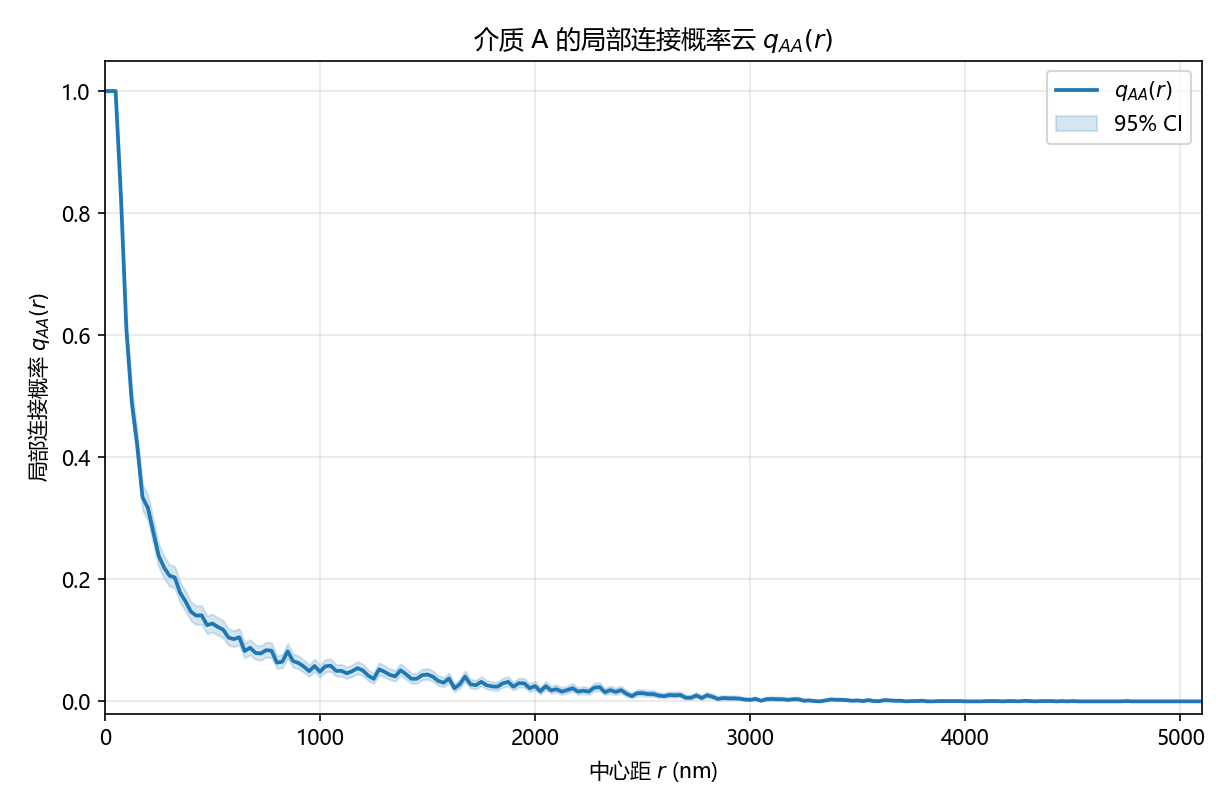
\includegraphics[width=0.75\textwidth]{version_log/2.0.0/conductive_microstructure/results/figures/problem2_q_aa.png}
    \caption{介质 A 的局部连接概率云 $q_{AA}(r)$。当中心距较小时两根圆柱几乎必连接，随着中心距增加，连接概率快速下降并形成长尾。}
    \label{fig:q2_qaa}
\end{figure}

\begin{figure}[htbp]
    \centering
    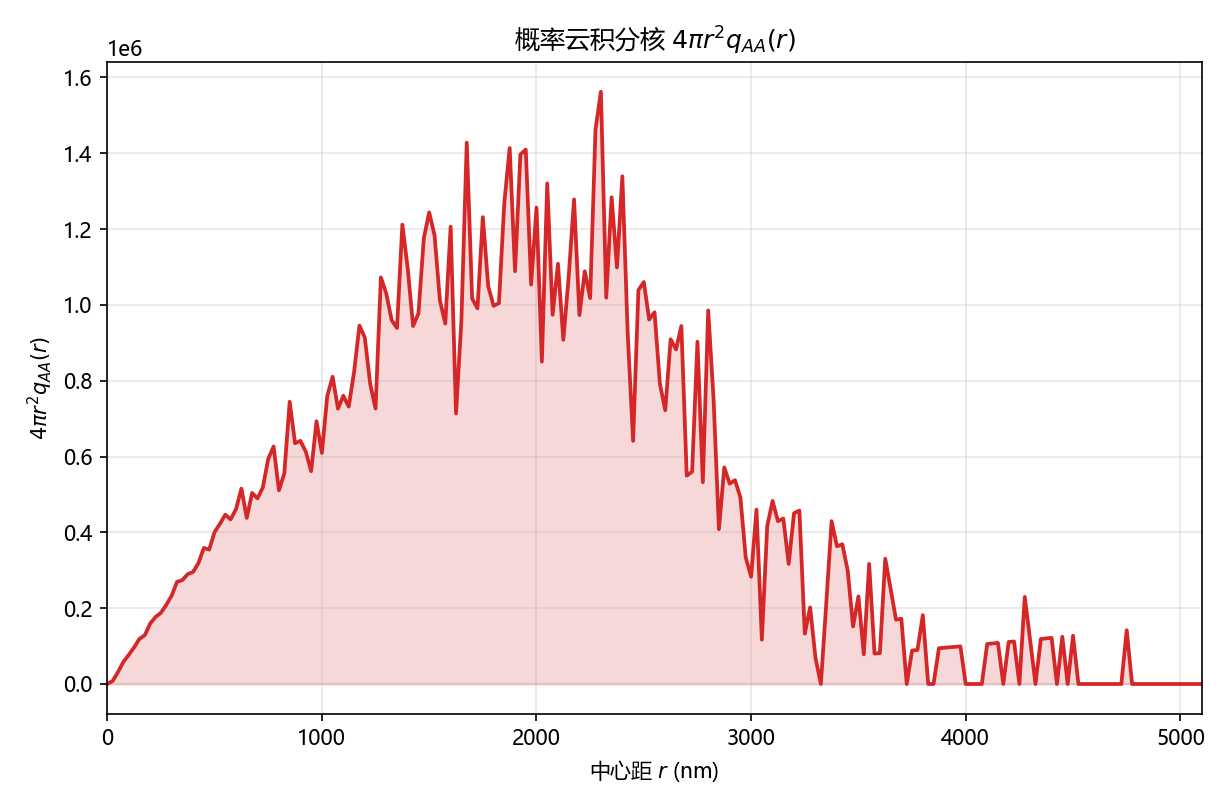
\includegraphics[width=0.75\textwidth]{version_log/2.0.0/conductive_microstructure/results/figures/problem2_4pir2q.png}
    \caption{概率云积分核 $4\pi r^2 q_{AA}(r)$。该曲线对 $r$ 的积分即为等效连接体积 $V_{AA}$。}
    \label{fig:q2_4pir2q}
\end{figure}

\subsection{Monte Carlo 贯通概率仿真}

对每组参数 $(\phi,\text{boundary mode})$，随机生成 $N_A$ 根圆柱并在边界回绕后切分为在箱片段；随后利用 AABB 宽相位筛选候选片段对，结合精确判距建立随机几何图，再判断左右电极是否连通。重复多次试验后，以
\[
\hat{P}_{\mathrm{conn}}=\frac{\text{贯通次数}}{\text{试验总次数}}
\]
估计导通概率，并给出 Wilson $95\%$ 置信区间。

\subsection{问题 2 结果与理论验证}

在 $\phi\in\{0.50\%,0.60\%,0.70\%,1.00\%\}$ 下得到的结果如表 \ref{tab:q2_result} 所示。

\begin{table}[htbp]
    \centering
    \caption{问题 2 在不同体积分数下的导通概率结果}
    \label{tab:q2_result}
    \begin{tabular}{ccccc}
        \hline
        $\phi(\%)$ & $N_A$ & 周期连续 $\hat{P}_{\mathrm{conn}}$ & 仅几何回绕 $\hat{P}_{\mathrm{conn}}$ & $\bar{k}$ \\
        \hline
        0.50 & 354 & 0.9150 & 0.9180 & 0.902 \\
        0.60 & 424 & 0.9505 & 0.9575 & 1.081 \\
        0.70 & 495 & 0.9750 & 0.9765 & 1.262 \\
        1.00 & 707 & 0.9965 & 0.9970 & 1.802 \\
        \hline
    \end{tabular}
\end{table}

结果显示：随着体积分数增加，系统导通概率单调上升；两种边界模式下的差异均小于 $0.7\%$，说明对于随机填充体系，边界解释对总体结论影响较小。更重要的是，当 $\bar{k}$ 从 $0.90$ 增加到 $1.08$ 时，导通概率恰好由“刚过 $90\%$ 阈值”跃升至接近 $95\%$。这说明：
\begin{quote}
    概率云给出的平均连接度 $\bar{k}$ 能有效刻画局部连接能力，并能正确预测宏观导通从临界区向高概率贯通区的转变趋势。
\end{quote}
与此同时，最大连通分量占比 $S_{\max}/N$ 也随体积分数单调升高：在 $\phi=0.50\%$ 时，两种边界模式下已分别达到 $0.9057$ 与 $0.9333$；到 $\phi=1.00\%$ 时则上升至 $0.9829$ 与 $0.9888$。这说明在临界区附近，网络并不是由大量彼此分离的小团簇组成，而是已经形成占主导地位的连通骨架。

因此，问题 2 为后续问题 3 和问题 4 提供了坚实的理论基础：概率云模型不仅可以解释仿真结果，而且可以作为后续优化搜索的理论先导。

\begin{figure}[htbp]
    \centering
    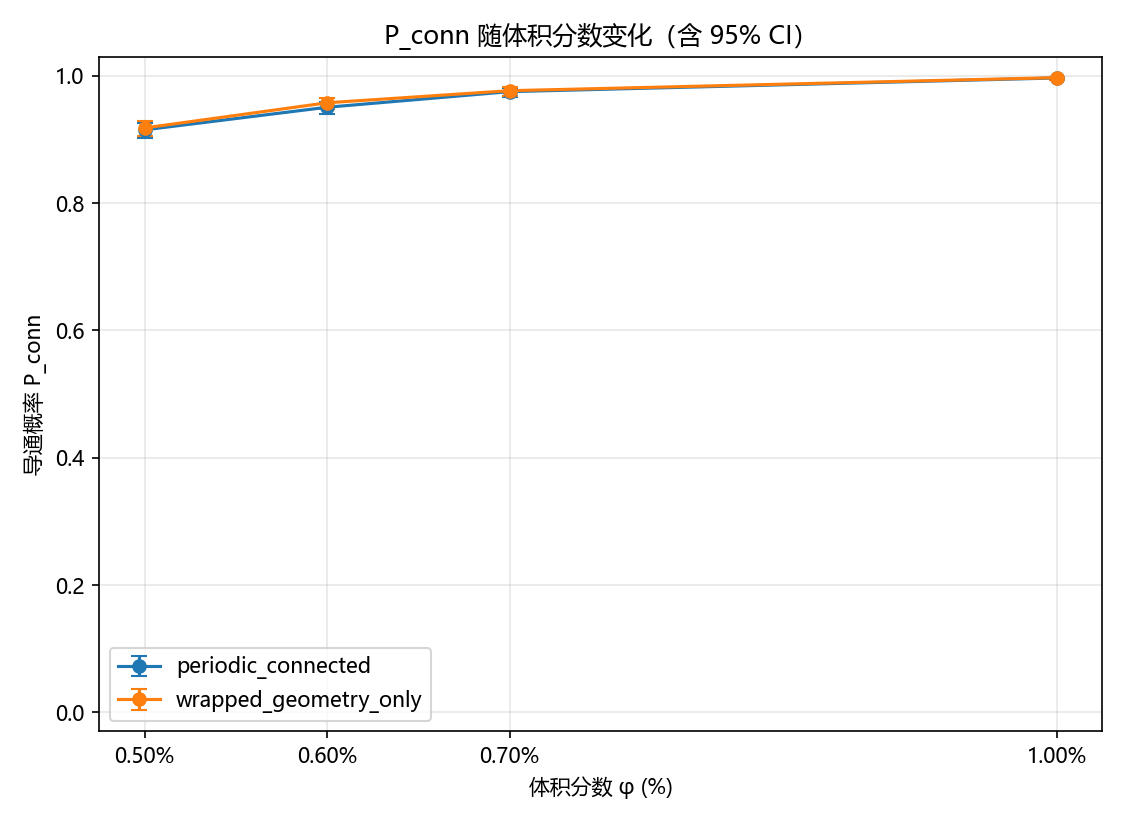
\includegraphics[width=0.72\textwidth]{version_log/2.0.0/conductive_microstructure/results/figures/problem2_p_conn.png}
    \caption{问题 2 中导通概率 $P_{\mathrm{conn}}$ 随体积分数 $\phi$ 的变化，两种边界模式下结果均随 $\phi$ 增大而单调上升。}
    \label{fig:q2_pconn}
\end{figure}

\begin{figure}[htbp]
    \centering
    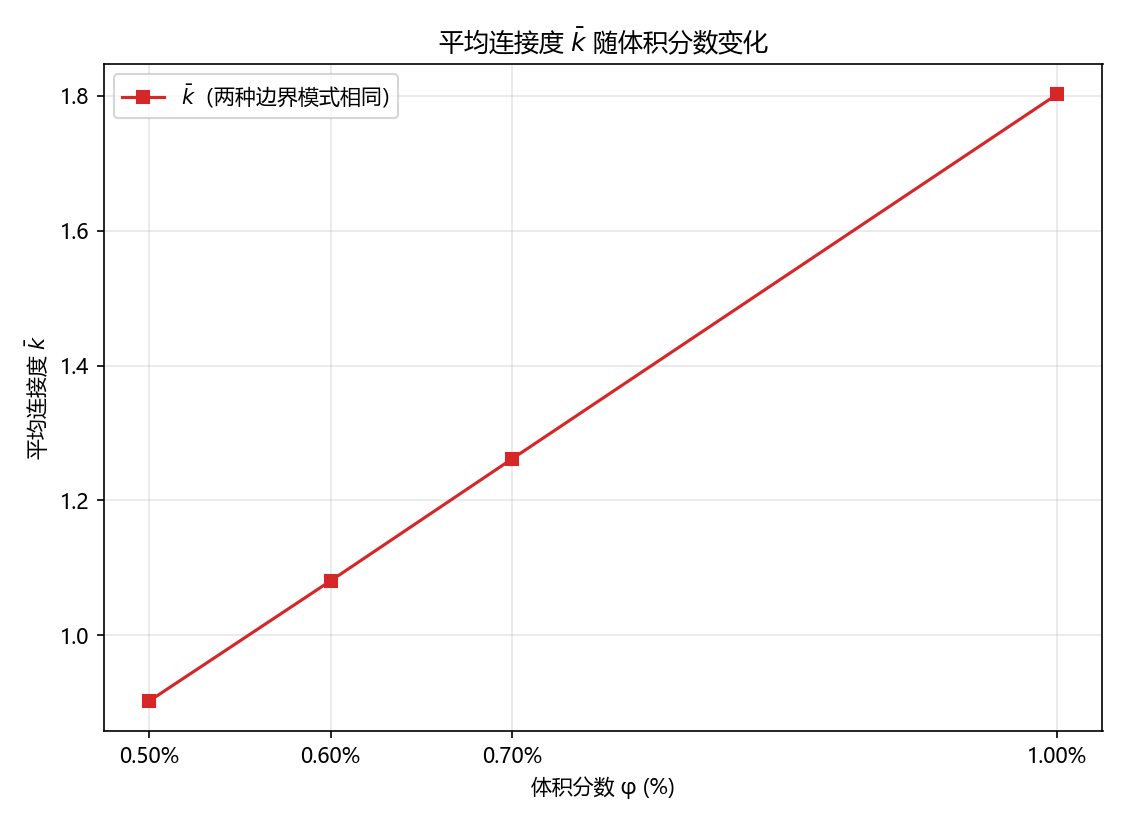
\includegraphics[width=0.72\textwidth]{version_log/2.0.0/conductive_microstructure/results/figures/problem2_kbar.png}
    \caption{问题 2 中概率云理论平均连接度 $\bar{k}$ 随体积分数 $\phi$ 的变化。随着填充率增加，单个节点的平均连接能力随之增强。}
    \label{fig:q2_kbar}
\end{figure}

\begin{figure}[htbp]
    \centering
    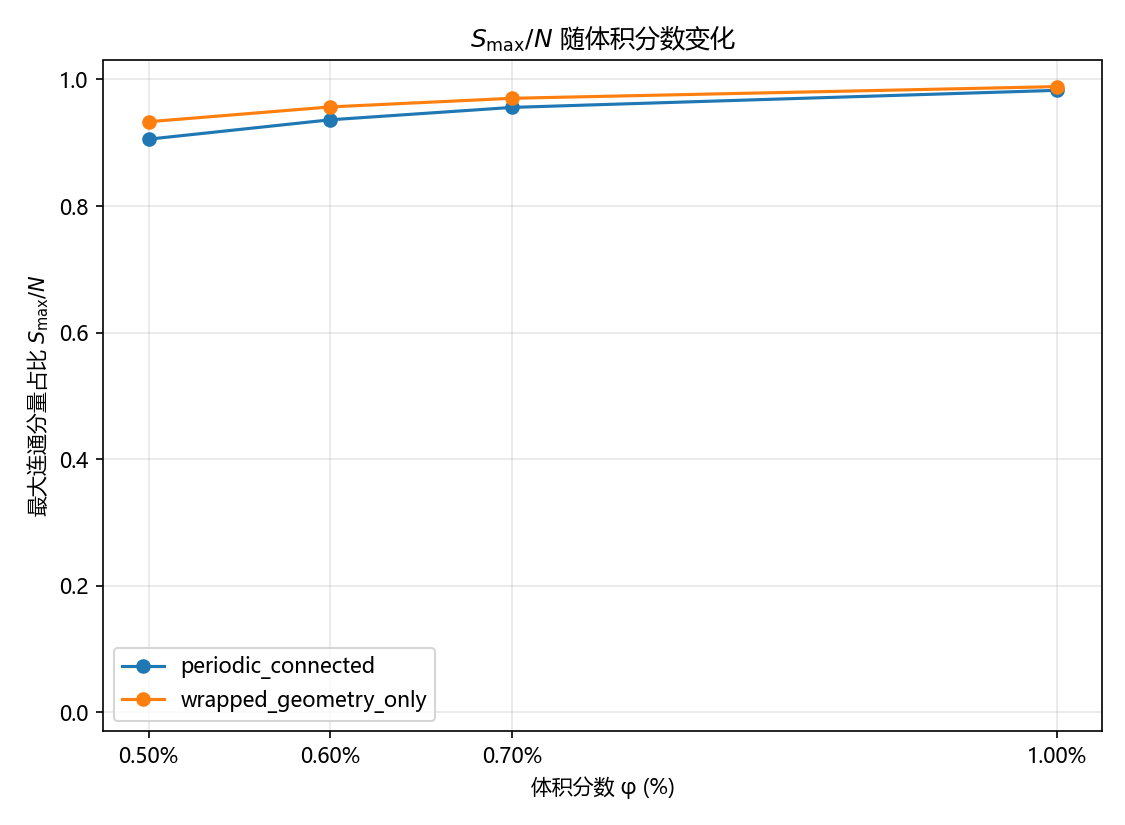
\includegraphics[width=0.72\textwidth]{version_log/2.0.0/conductive_microstructure/results/figures/problem2_smax_ratio.png}
    \caption{问题 2 中最大连通分量占比 $S_{\max}/N$ 随体积分数 $\phi$ 的变化。该指标反映了网络从分散小团簇向主导连通骨架演化的过程。}
    \label{fig:q2_smax}
\end{figure}

\begin{figure}[htbp]
    \centering
    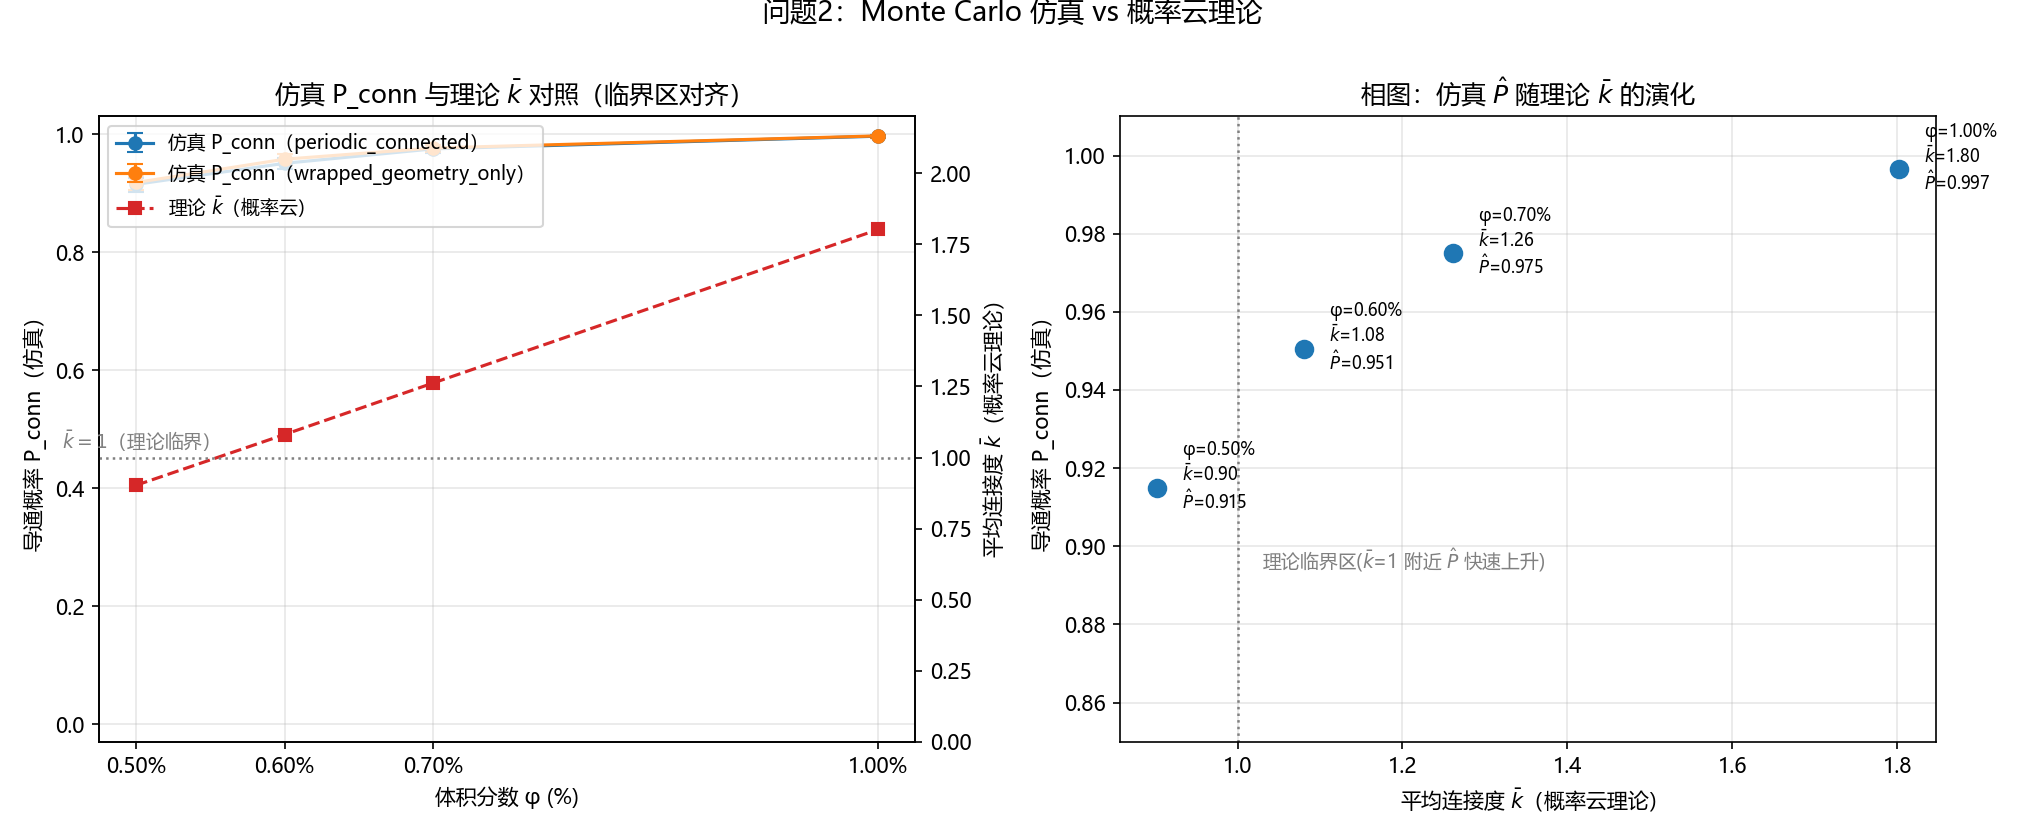
\includegraphics[width=0.92\textwidth]{version_log/2.0.0/conductive_microstructure/results/figures/problem2_theory_vs_simulation.png}
    \caption{问题 2 中 Monte Carlo 仿真与概率云理论的对照。左图展示导通概率与平均连接度随体积分数的变化，右图给出 $\hat{P}_{\mathrm{conn}}$ 与 $\bar{k}$ 的对应关系。}
    \label{fig:q2_theory_vs_sim}
\end{figure}

\section{问题 3：满足 \texorpdfstring{$P_{\mathrm{conn}}\ge 90\%$}{Pconn>=90\%} 的最低填充率}

\subsection{二分搜索与单侧置信判据}

问题 3 的目标是求满足
\[
P_{\mathrm{conn}}\ge 0.90
\]
时介质 A 的最低体积分数 $\phi_{\min}$。由于填充率越大，体系整体连边越多，贯通概率总体上单调不减，因此可在区间
\[
[\phi_{\mathrm{low}},\phi_{\mathrm{high}}]=[0.20\%,0.70\%]
\]
上采用二分搜索。

为了避免仅凭点估计作出过于乐观的判断，本文使用 Wilson 单侧 $95\%$ 置信下界
\[
p_{\mathrm{lower},95\%}\ge 0.90
\]
作为“达标”的统计判据。若直接使用 $\hat{P}_{\mathrm{conn}}\ge 0.90$，则在真实概率恰处于临界附近时，容易因抽样波动而误判；而采用单侧置信下界可以保证结论更稳健。

\subsection{理论临界值}

由问题 2 已得
\[
V_{AA}=2.5493\times 10^9\,\mathrm{nm}^3.
\]
令平均连接度满足
\[
\bar{k}=1,
\]
即可得到理论临界填充率
\[
\phi_{\mathrm{theory}}=\frac{V_A}{V_{AA}}\approx 0.005546=0.5546\%.
\]
这并不是“$90\%$ 导通”的精确解析公式，而是一个用于描述渗流临界位置的理论参考值。

\subsection{问题 3 结果}

在二分中点使用 $1000$ 次试验判定，收敛后对候选点使用 $4000$ 次试验复核，得到表 \ref{tab:q3_result}。

\begin{table}[htbp]
    \centering
    \caption{问题 3 的最低填充率结果}
    \label{tab:q3_result}
    \begin{tabular}{cccccc}
        \hline
        边界模式 & $\phi_{\min}$ & $N_A$ & $\hat{P}_{\mathrm{conn}}$ & $p_{\mathrm{lower},95\%}$ & $\phi_{\mathrm{theory}}$ \\
        \hline
        周期连续 & 0.5125\% & 363 & 0.9155 & 0.9080 & 0.5546\% \\
        仅几何回绕 & 0.4969\% & 351 & 0.9075 & 0.8997 & 0.5546\% \\
        \hline
    \end{tabular}
\end{table}

可以看到，两种模式下的最低填充率都落在 $0.50\%$ 附近，且略低于理论临界值 $0.5546\%$。这表明概率云理论给出的临界参考与真实仿真结果在量级和变化方向上是一致的。其偏低的原因在于：介质 A 长径比较大，链式连接能力较强，因此在有限尺寸盒体中，达到 $90\%$ 贯通概率时所需的体积分数可以略低于均值场意义下的 $\bar{k}=1$ 临界点。

需要如实说明的是，\texttt{wrapped\_geometry\_only} 模式下最终 $4000$ 次复核得到
\[
p_{\mathrm{lower},95\%}=0.8997,
\]
略低于 $0.90$。这说明该点位于统计临界附近，属于由有限样本波动带来的边界现象，而不是模型失效。相较于问题 2 的趋势验证，问题 3 进一步给出了概率云理论与实际临界填充率之间的定量对应关系。

\begin{figure}[htbp]
    \centering
    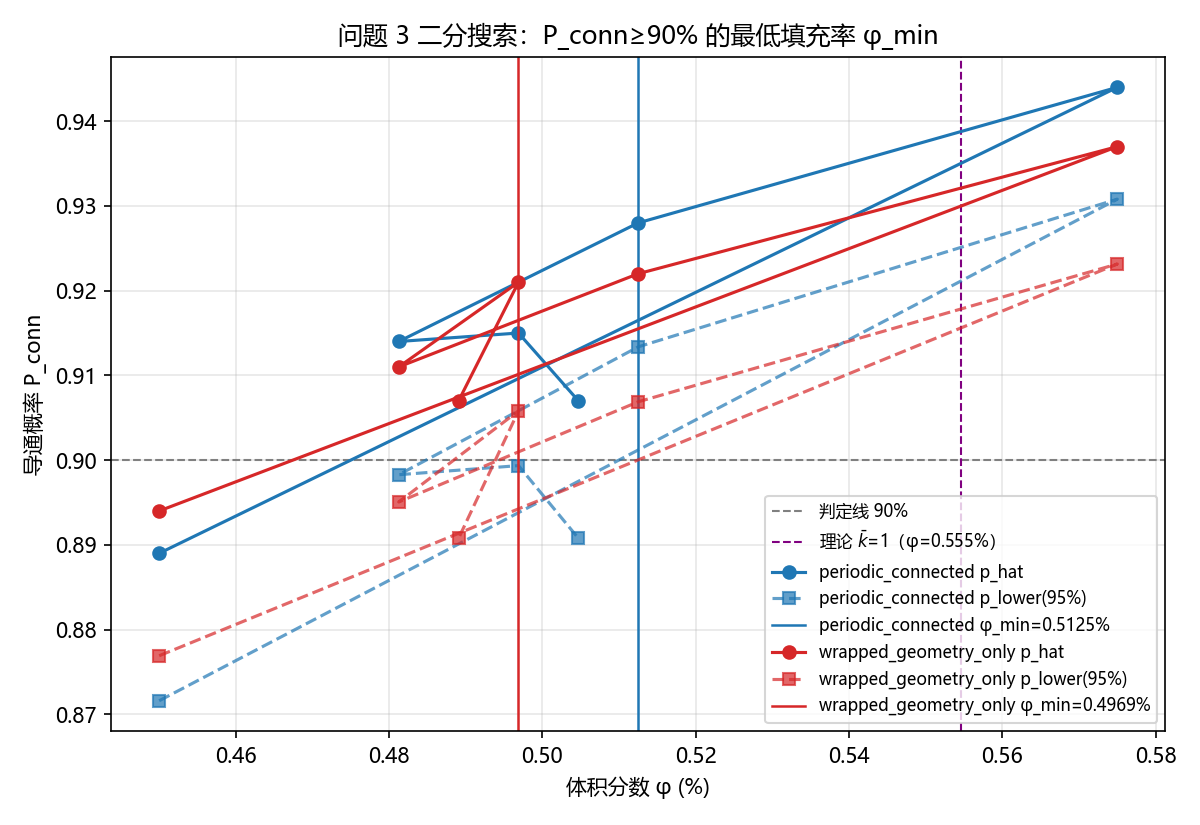
\includegraphics[width=0.72\textwidth]{version_log/2.0.0/conductive_microstructure/results/problem3/problem3_bisection.png}
    \caption{问题 3 中最低填充率的二分搜索过程示意图。图中展示了不同候选填充率下的判定结果及最终收敛区间。}
    \label{fig:q3_bisection}
\end{figure}

\section{问题 4：A/B 混合体系的最低成本组合}

\subsection{A/B 混合导通判据与成本函数}

在问题 4 中，除介质 A 外引入介质 B。其球心均匀分布在
\[
[-4800,4800]^3
\]
内，以保证球体完全落在盒内。混合体系的导通判据为：
\[
d_{AA}\le 61.8\,\mathrm{nm},\qquad
d_{AB}\le 231.8\,\mathrm{nm},\qquad
d_{BB}\le 401.8\,\mathrm{nm},
\]
且 B 球与电极平面导通的条件为球面到平面距离不超过 $\delta$，对应球心到电极面的距离阈值为 $201.8\,\mathrm{nm}$。

总成本函数写为
\[
C(N_A,N_B)=1.05\cdot N_A\frac{V_A}{10^9}+0.05\cdot N_B\frac{V_B}{10^9},
\]
其中
\[
V_B=\frac{4}{3}\pi R_B^3\approx 3.351\times 10^7\,\mathrm{nm}^3.
\]
目标是在
\[
P_{\mathrm{conn}}\ge 0.90
\]
的约束下，使成本最小。

\subsection{双介质概率云与连接矩阵}

在问题 2 的概率云思想基础上，定义混合体系中的三种等效连接体积：
\[
V_{AA},\qquad V_{AB},\qquad V_{BB}.
\]
其中 $V_{AA}$ 由问题 2 已得；$V_{BB}$ 可解析计算为半径 $401.8\,\mathrm{nm}$ 球体的体积；$V_{AB}$ 通过采样 A 的方向与 B 相对位置方向后数值积分得到。本文计算结果为
\[
V_{AA}=2.5493\times 10^9\,\mathrm{nm}^3,
\]
\[
V_{AB}=9.0877\times 10^8\,\mathrm{nm}^3,
\]
\[
V_{BB}=2.7172\times 10^8\,\mathrm{nm}^3.
\]
进一步构造连接矩阵
\[
M=
\begin{bmatrix}
\rho_A V_{AA} & \rho_B V_{AB}\\
\rho_A V_{AB} & \rho_B V_{BB}
\end{bmatrix},
\]
并以其最大特征值 $\lambda_{\max}$ 作为理论可行区的筛选指标。

\subsection{三级搜索策略}

问题 4 的求解采用“理论筛选 + Monte Carlo 边界搜索 + 成本优化确认”的三级流程：
\begin{enumerate}
    \item 在 $(N_A,N_B)$ 网格上扫描 $\lambda_{\max}$，得到理论可行区；
    \item 对每个 $N_A$ 网格点，在 $N_B\in[0,5000]$ 上用整数二分搜索满足 $p_{\mathrm{lower},95\%}\ge 0.90$ 的最小 $N_B$，得到可行边界；
    \item 沿边界计算成本，选取最小成本候选，并在其邻域用 $4000$ 次试验复核，最终确定最优解。
\end{enumerate}
之所以采用这种流程，是因为纯粹二维暴力扫描计算量极大，而理论可行区能够显著缩小需要精细仿真的范围。

\subsection{问题 4 结果与经济解释}

最终得到的最优解如表 \ref{tab:q4_result} 所示。

\begin{table}[htbp]
    \centering
    \caption{问题 4 的最低成本组合结果}
    \label{tab:q4_result}
    \begin{tabular}{cccccc}
        \hline
        边界模式 & $N_A^\ast$ & $N_B^\ast$ & 最低成本/元 & $\hat{P}_{\mathrm{conn}}$ & $p_{\mathrm{lower},95\%}$ \\
        \hline
        周期连续 & 360 & 0  & 5.3438 & 0.9147 & 0.9072 \\
        仅几何回绕 & 340 & 50 & 5.1307 & 0.9095 & 0.9018 \\
        \hline
    \end{tabular}
\end{table}

与此同时，理论层给出的 $\lambda_{\max}\ge 1$ 可行区为
\[
N_A\in[0,360],\qquad N_B\in[400,5000].
\]
与 Monte Carlo 实际边界相比，理论可行区明显偏宽松，但两者在趋势上是一致的：随着 $N_A$ 增大，所需的 $N_B$ 总体下降。这说明连接矩阵仍然成功刻画了局部连接能力的变化方向，只是有限尺寸下的实际贯通要求比均值场阈值更严格。

从工程解释看，最重要的结论不是“B 球越多越好”，而是：
\begin{quote}
    最低成本方案始终以介质 A 为主，介质 B 仅在临界区起到少量桥接补强作用。
\end{quote}
这是因为 B 球虽然单位体积成本较低，但单颗粒体积较大、点接触导电效率不如细长圆柱高；因此若试图依靠大量 B 球单独建立贯通路径，成本反而更高。只有当 A 已经接近形成主骨架时，加入少量 B 球才具有明显的边际收益。

\begin{figure}[htbp]
    \centering
    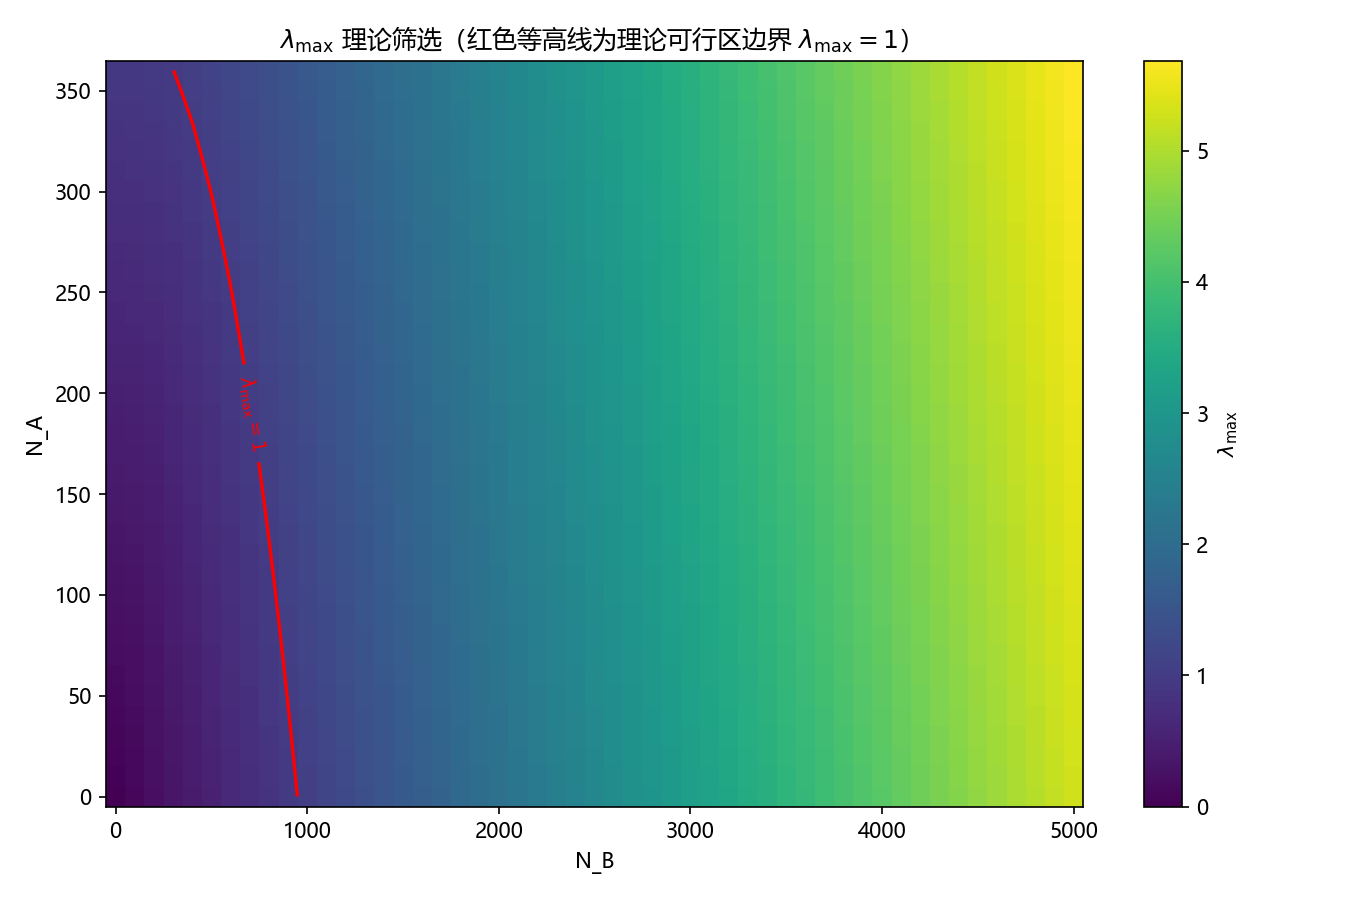
\includegraphics[width=0.78\textwidth]{version_log/2.0.0/conductive_microstructure/results/problem4/problem4_lambda_max_heatmap.png}
    \caption{问题 4 中 A/B 混合体系的 $\lambda_{\max}$ 理论热图。红色等高线对应 $\lambda_{\max}=1$，用于给出理论可行区。}
    \label{fig:q4_lambda}
\end{figure}

\begin{figure}[htbp]
    \centering
    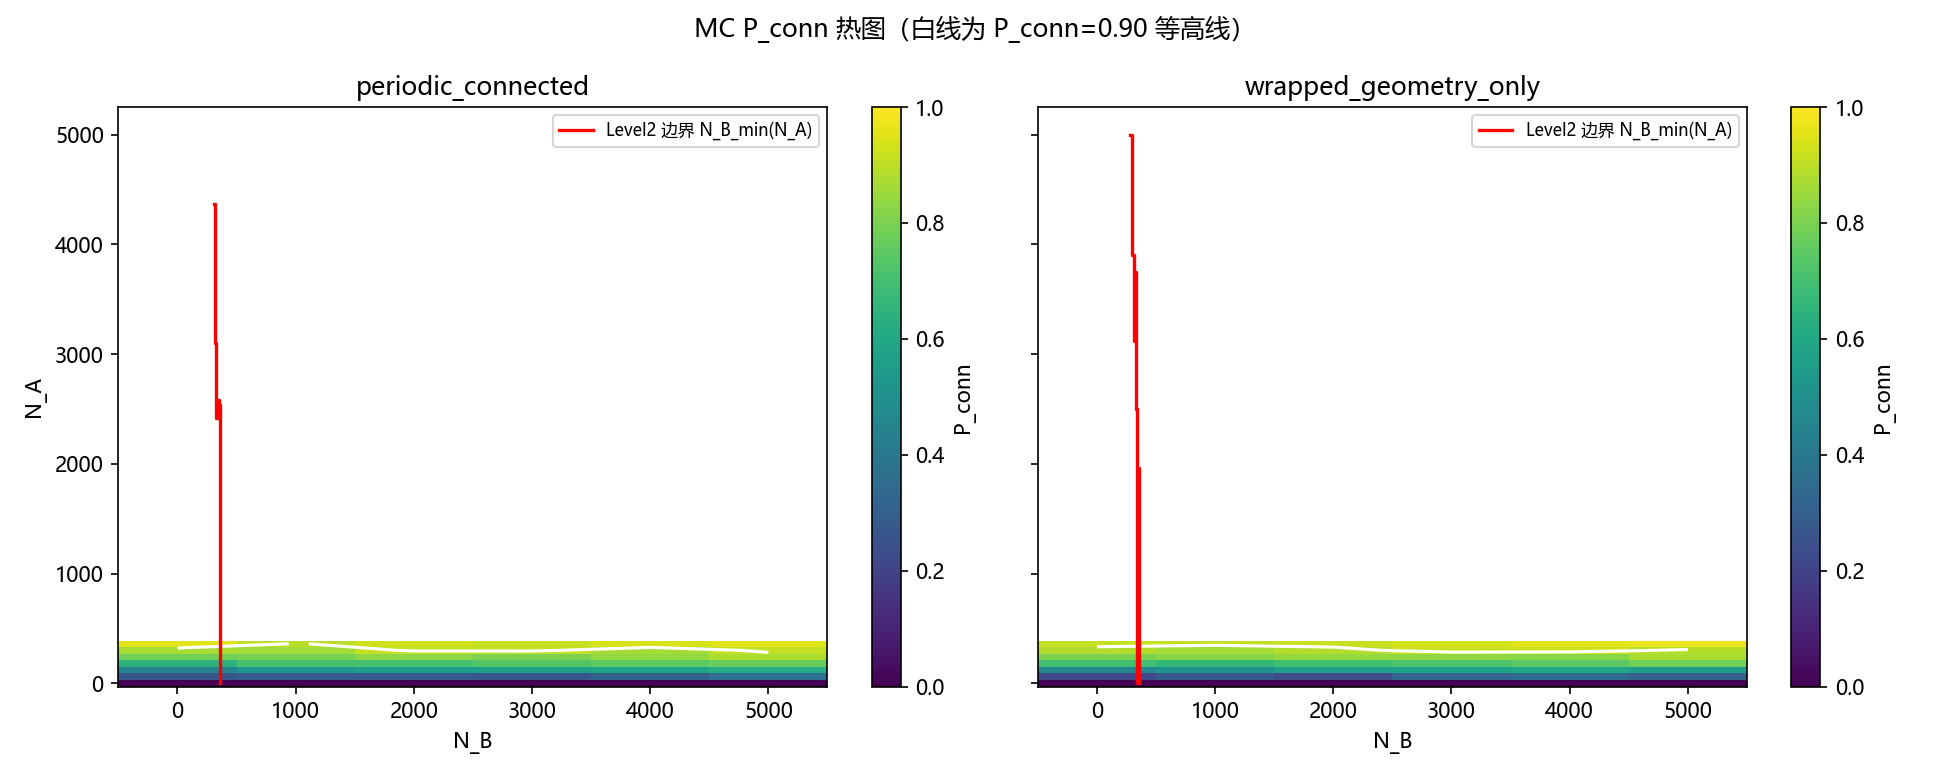
\includegraphics[width=0.92\textwidth]{version_log/2.0.0/conductive_microstructure/results/problem4/problem4_mc_pconn_heatmap.png}
    \caption{问题 4 中 A/B 混合体系的 Monte Carlo 导通概率热图。白色等高线为 $P_{\mathrm{conn}}=0.90$，红色阶梯线为二分搜索得到的可行边界。}
    \label{fig:q4_mc_heatmap}
\end{figure}

\begin{figure}[htbp]
    \centering
    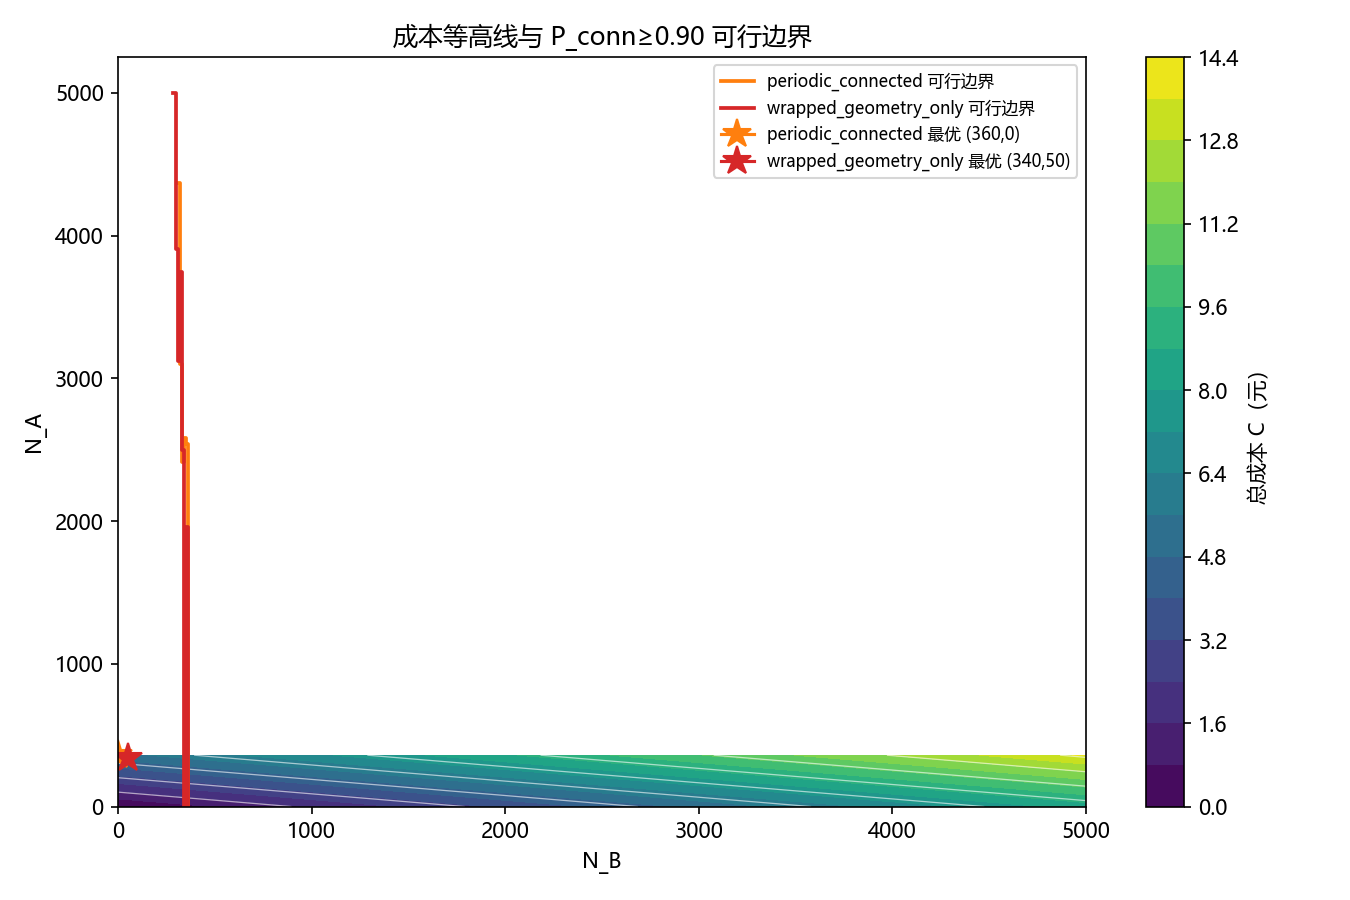
\includegraphics[width=0.78\textwidth]{version_log/2.0.0/conductive_microstructure/results/problem4/problem4_cost_boundary.png}
    \caption{问题 4 中成本等高线与可行边界。图中标出了满足 $P_{\mathrm{conn}}\ge 0.90$ 的最优组合位置。}
    \label{fig:q4_cost_boundary}
\end{figure}

\section{模型评价与结论}

\subsection{模型优点}

本文模型的主要优点体现在以下三个方面：
\begin{enumerate}
    \item 建立了统一的求解框架。问题 1 到问题 4 并非彼此割裂，而是围绕“局部连接 -- 宏观贯通 -- 优化决策”逐层展开；
    \item 理论与仿真互相支撑。概率云和连接矩阵负责解释渗流趋势与缩小搜索范围，Monte Carlo 负责给出有限尺寸盒体中的最终贯通概率；
    \item 结果具有较强可复现性。问题 3 的跨设备独立复现结果逐字节一致，说明当前随机种子派生和评估顺序设计可靠。
\end{enumerate}

\subsection{模型局限}

本文也存在以下局限：
\begin{enumerate}
    \item 圆柱之间的导通判据采用 capsule 近似，在端面附近存在微小几何误差；
    \item 概率云和连接矩阵基于各向同性随机分布的统计假设，未显式处理可能存在的取向偏置；
    \item 当前结论严格对应于题目给定的盒体尺度、几何参数和导通阈值，属于有限尺寸体系的工程结论。
\end{enumerate}

\subsection{全文结论}

综合问题 1 至问题 4 的结果，可以得到以下总体结论：
\begin{enumerate}
    \item 基于几何判距、边界处理和随机几何图的导通判定框架能够稳定刻画微构体中的导电贯通行为；
    \item 由局部连接概率云得到的等效连接体积与平均连接度，能够有效解释介质 A 体系中导通概率随填充率上升的规律；
    \item 满足 $P_{\mathrm{conn}}\ge 0.90$ 时，介质 A 的最低填充率约为 $0.50\%$，与理论临界值 $0.5546\%$ 同量级且方向一致，说明概率云理论已得到充分数值验证；
    \item 在 A/B 混合体系中，满足 $P_{\mathrm{conn}}\ge 0.90$ 的最低成本方案并不是以 B 为主体，而是以 A 为主、B 为辅的混合策略。
\end{enumerate}

因此，本文建立的“几何导通判据 -- 概率云 -- 渗流解释 -- Monte Carlo 验证 -- 优化求解”方法链，对微构体填充导电介质问题具有较好的统一解释能力和求解能力。

\section*{图表与结果文件对应说明}

正文涉及的主要图表可与现有结果文件对应如下。

公共目录：\texttt{version\_log/2.0.0/conductive\_microstructure/results/}

具体文件清单：
\begin{itemize}
    \small
    \item 问题 2 概率云图：\texttt{figures/problem2\_q\_aa.png}
    \item 问题 2 概率云积分核图：\texttt{figures/problem2\_4pir2q.png}
    \item 问题 2 导通概率图：\texttt{figures/problem2\_p\_conn.png}
    \item 问题 2 平均连接度图：\texttt{figures/problem2\_kbar.png}
    \item 问题 2 最大连通分量占比图：\texttt{figures/problem2\_smax\_ratio.png}
    \item 问题 2 理论--仿真对照图：\texttt{figures/problem2\_theory\_vs\_simulation.png}
    \item 问题 3 二分结果图：\texttt{problem3/problem3\_bisection.png}
    \item 问题 4 理论热图：\texttt{problem4/problem4\_lambda\_max\_heatmap.png}
    \item 问题 4 Monte Carlo 热图：\texttt{problem4/problem4\_mc\_pconn\_heatmap.png}
    \item 问题 4 成本边界图：\texttt{problem4/problem4\_cost\_boundary.png}
\end{itemize}

\section*{参考文献}

\begin{thebibliography}{99}
    \bibitem{huashu2026} 2026 第七届“华数杯”大学生数学建模竞赛 A 题：微构体中填充导电介质的仿真优化.
    \bibitem{attachment} 竞赛附件：\texttt{附件.xlsx}.
    \bibitem{format} 2026 第七届华数杯数学建模竞赛论文格式规范与提交说明.
\end{thebibliography}

% 说明：本文件从正文部分开始，不包含标题页、摘要页、关键词页、承诺页等第一页内容。

\section{问题重述与建模目标}

题目研究边长为 $10000\,\mathrm{nm}$ 的立方体微构体中导电介质随机填充后的贯通行为。微构体区域记为
\[
\Omega=[-5000,5000]^3,\qquad V_0=10^{12}\,\mathrm{nm}^3.
\]
体系中包含两类导电介质：
\begin{itemize}
    \item 介质 A：直圆柱，长度 $L_A=5000\,\mathrm{nm}$，半径 $R_A=30\,\mathrm{nm}$；
    \item 介质 B：球体，半径 $R_B=200\,\mathrm{nm}$。
\end{itemize}
左右带电面取为垂直于 $X$ 轴的两个平面
\[
x=-5000,\qquad x=5000.
\]
当两个导电介质之间，或导电介质与电极之间的最短距离满足
\[
d\le \delta,\qquad \delta=1.8\,\mathrm{nm}
\]
时，认为二者电学导通。若左右电极之间存在至少一条由导电介质组成的完整连接路径，则称微构体导通。

本题的四个问题可以统一归纳为：在既定几何规则和随机分布假设下，如何从局部导通判据出发，建立能够解释宏观贯通行为并完成参数优化的模型。围绕这一目标，本文建立如下统一技术路线：
\[
\boxed{
\begin{aligned}
\text{几何导通判据}
&\rightarrow
\text{局部连接概率云}
\rightarrow
\text{等效连接体积}\\
&\rightarrow
\text{随机几何图/连续渗流解释}
\rightarrow
\text{Monte Carlo 验证}\\
&\rightarrow
\text{临界填充率与成本优化}
\end{aligned}
}
\]
其中，问题 1 解决确定性结构的导通判定，问题 2 研究给定填充率时的导通概率，问题 3 求满足 $P_{\mathrm{conn}}\ge 0.90$ 时介质 A 的最低填充率，问题 4 在 $P_{\mathrm{conn}}\ge 0.90$ 的约束下求 A/B 混合体系的最低成本组合。

\section{模型假设}

为建立明确的概率测度并保持模型可计算，作如下假设：
\begin{enumerate}
    \item 所有介质位置独立均匀分布于微构体内；
    \item 介质 A 姿态服从球面各向同性分布；
    \item 介质之间允许重叠和贯穿，不考虑排斥体积效应；
    \item 不考虑重力、动态重排及时间演化，系统视为静态随机结构；
    \item 最短距离不超过 $1.8\,\mathrm{nm}$ 即视为理想导通；
    \item 同一导电介质内部视为整体等势导体；
    \item 除题目给出的边界截断/回绕规则外，不额外引入表面效应；
    \item Monte Carlo 各次试验彼此独立。
\end{enumerate}

需要指出的是，第 1、2 条是建立导通概率模型的核心统计假设。本文中的概率云与连接矩阵用于描述\textbf{局部连接能力及渗流趋势}，有限尺寸微构体中沿电极方向的实际贯通概率最终仍由 Monte Carlo 仿真确定。因此，本文不作如下过强结论：$\bar{k}>1$ 时系统一定导通，或 $\lambda_{\max}>1$ 等价于 $90\%$ 导通。

\section{问题 1：三组确定性结构的导通判定}

\subsection{附件数据解释与边界模式}

附件 \texttt{附件.xlsx} 给出三组介质 A 的端点坐标数据，每行包含一根圆柱轴线段的两个端点。对数据核对后发现，附件中的部分轴线段长度小于 $5000\,\mathrm{nm}$，且存在多行端点在周期回绕后完全重合、长度和恰好为 $5000\,\mathrm{nm}$ 的现象。这说明附件中的一行并不总是完整圆柱，而可能是\textbf{经过边界截断后的在箱片段}。

因此，对边界规则作两种解释并分别计算：
\begin{enumerate}
    \item \texttt{PERIODIC\_CONNECTED}：跨边界后仍视为同一根导体，周期回绕后重合的片段合并为同一节点；
    \item \texttt{WRAPPED\_GEOMETRY\_ONLY}：仅做几何回绕，每一行数据都视为独立节点，不承认跨边界电学连续。
\end{enumerate}
这种双模式处理既保留了题目描述下的物理解释，也便于后续做敏感性分析。

\subsection{几何导通判据与建图}

将圆柱体用 capsule 近似表示为“轴线段向外膨胀半径 $R_A$”得到的几何体，则两根介质 A 导通的条件为
\[
d_{\mathrm{seg}} \le 2R_A+\delta = 61.8\,\mathrm{nm},
\]
其中 $d_{\mathrm{seg}}$ 为两条轴线段最短距离。介质 A 与电极平面导通条件为
\[
d_{\mathrm{axis\mbox{-}plane}} \le R_A+\delta = 31.8\,\mathrm{nm}.
\]
在计算实现中，先根据边界模式构造节点，再依据圆柱--圆柱和圆柱--电极的导通判据建立无向图，最后通过并查集和多源 BFS 判断左右电极是否处于同一连通分量并提取一条贯通路径。

\subsection{问题 1 结果与解释}

三组数据的判定结果如表 \ref{tab:q1_result} 所示。

\begin{table}[htbp]
    \centering
    \caption{问题 1 三组结构的导通判定结果}
    \label{tab:q1_result}
    \begin{tabular}{cccc}
        \hline
        分组 & 数据行数 & \texttt{PERIODIC\_CONNECTED} & \texttt{WRAPPED\_GEOMETRY\_ONLY} \\
        \hline
        组1 & 12  & 导通 & 不导通 \\
        组2 & 49  & 导通 & 导通 \\
        组3 & 535 & 导通 & 导通 \\
        \hline
    \end{tabular}
\end{table}

进一步统计表明，周期连续模式下组 1 的 12 行数据会被合并为 9 个节点，组 2 的 49 行会被合并为 39 个节点，组 3 的 535 行会被合并为 357 个节点。这说明附件数据中确实存在大量被边界截断后拆开的圆柱片段。

这一问的主要意义不在于三组结果本身，而在于为后续随机填充问题建立了一个可靠的几何基线：\textbf{边界处理方式、圆柱判距方法、建图与贯通判定框架已经得到验证}。其中，组 1 在两种边界解释下结论不同，恰好说明边界规则可能对个别确定性结构敏感；而组 2、组 3 在两种模式下均导通，说明其贯通性更为稳健。

\section{问题 2：给定填充率时的导通概率}

\subsection{随机生成模型}

对问题 2，仅考虑介质 A 的随机填充。设其体积分数为 $\phi$，则圆柱数目取为
\[
N_A=\mathrm{round}\!\left(\frac{\phi V_0}{V_A}\right),\qquad
V_A=\pi R_A^2L_A\approx 1.4137\times 10^7\,\mathrm{nm}^3.
\]
圆柱中心在盒内均匀分布，方向采用球面均匀采样。为避免极区聚集，不直接令极角 $\theta\sim U(0,\pi)$，而采用
\[
z=\cos\theta\sim U(-1,1),\qquad \varphi\sim U(0,2\pi),
\]
从而保证方向关于立体角均匀。

\subsection{局部连接概率云与等效连接体积}

固定两根介质 A 的中心距为 $r$，并令两根圆柱方向独立球面均匀，则定义径向连接概率云
\[
q_{AA}(r)=P(\text{两根 A 导通}\mid \text{中心距为 }r).
\]
对应的等效连接体积定义为
\[
V_{AA}=4\pi\int_0^\infty r^2 q_{AA}(r)\,\mathrm{d}r.
\]
本文通过 Monte Carlo 对 $q_{AA}(r)$ 逐点采样，再用数值积分得到
\[
V_{AA}=2.5493\times 10^9\,\mathrm{nm}^3.
\]
进一步定义平均连接度
\[
\bar{k}=\rho_A V_{AA},\qquad \rho_A=\frac{N_A}{V_0}.
\]
它反映了随机体系中单个节点的平均连接能力，可用于解释渗流临界附近的宏观行为变化。

\begin{figure}[htbp]
    \centering
    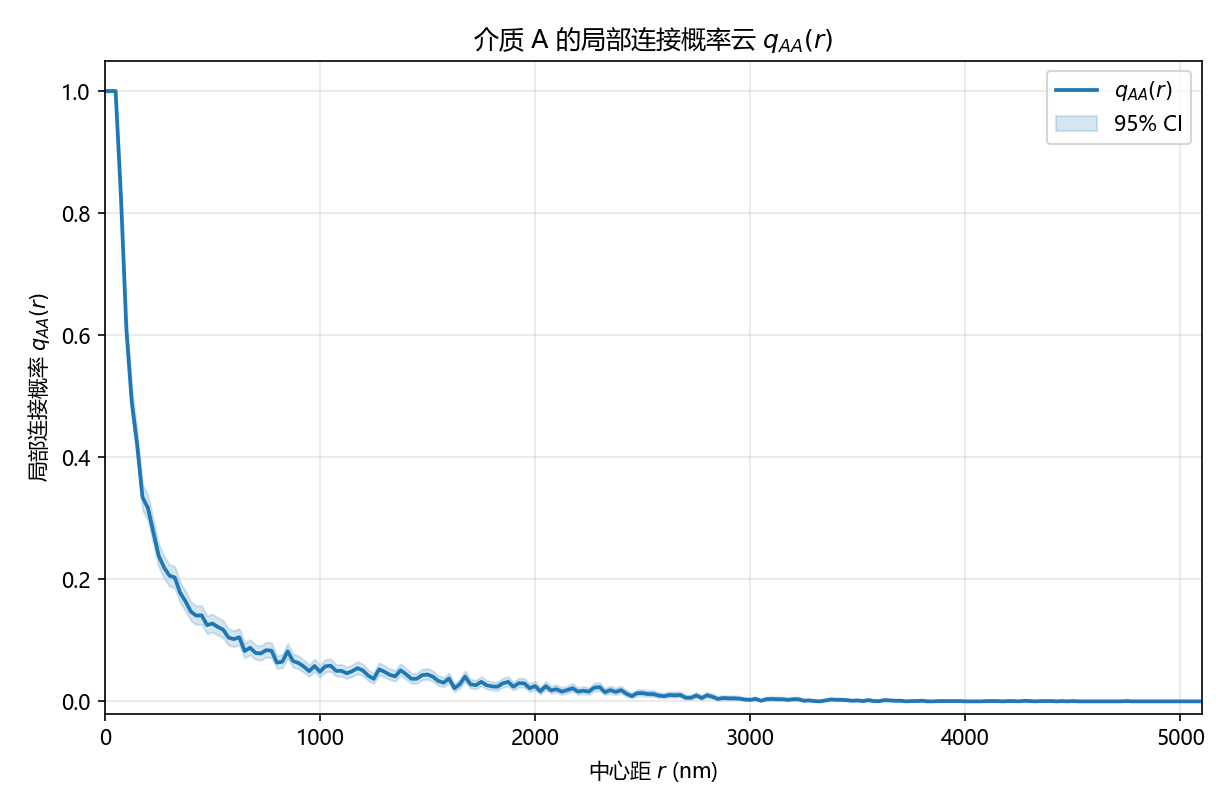
\includegraphics[width=0.75\textwidth]{version_log/2.0.0/conductive_microstructure/results/figures/problem2_q_aa.png}
    \caption{介质 A 的局部连接概率云 $q_{AA}(r)$。当中心距较小时两根圆柱几乎必连接，随着中心距增加，连接概率快速下降并形成长尾。}
    \label{fig:q2_qaa}
\end{figure}

\begin{figure}[htbp]
    \centering
    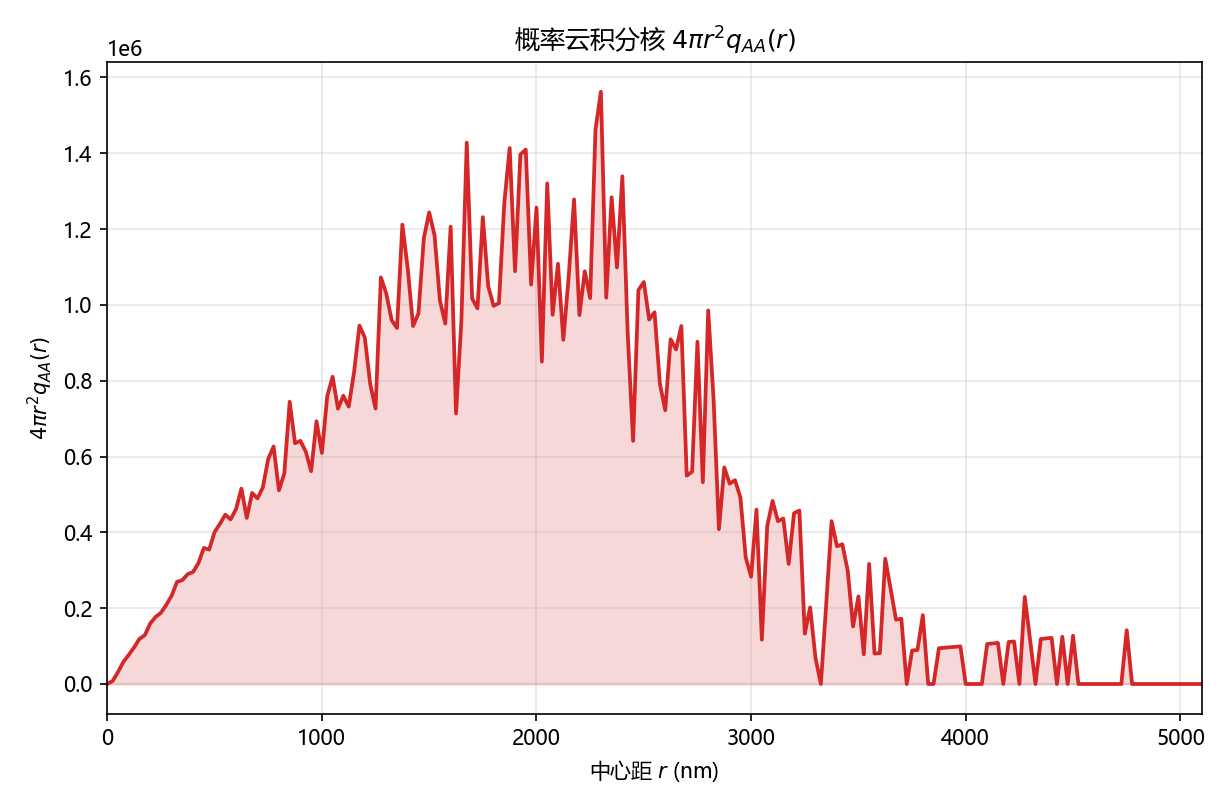
\includegraphics[width=0.75\textwidth]{version_log/2.0.0/conductive_microstructure/results/figures/problem2_4pir2q.png}
    \caption{概率云积分核 $4\pi r^2 q_{AA}(r)$。该曲线对 $r$ 的积分即为等效连接体积 $V_{AA}$。}
    \label{fig:q2_4pir2q}
\end{figure}

\subsection{Monte Carlo 贯通概率仿真}

对每组参数 $(\phi,\text{boundary mode})$，随机生成 $N_A$ 根圆柱并在边界回绕后切分为在箱片段；随后利用 AABB 宽相位筛选候选片段对，结合精确判距建立随机几何图，再判断左右电极是否连通。重复多次试验后，以
\[
\hat{P}_{\mathrm{conn}}=\frac{\text{贯通次数}}{\text{试验总次数}}
\]
估计导通概率，并给出 Wilson $95\%$ 置信区间。

\subsection{问题 2 结果与理论验证}

在 $\phi\in\{0.50\%,0.60\%,0.70\%,1.00\%\}$ 下得到的结果如表 \ref{tab:q2_result} 所示。

\begin{table}[htbp]
    \centering
    \caption{问题 2 在不同体积分数下的导通概率结果}
    \label{tab:q2_result}
    \begin{tabular}{ccccc}
        \hline
        $\phi(\%)$ & $N_A$ & 周期连续 $\hat{P}_{\mathrm{conn}}$ & 仅几何回绕 $\hat{P}_{\mathrm{conn}}$ & $\bar{k}$ \\
        \hline
        0.50 & 354 & 0.9150 & 0.9180 & 0.902 \\
        0.60 & 424 & 0.9505 & 0.9575 & 1.081 \\
        0.70 & 495 & 0.9750 & 0.9765 & 1.262 \\
        1.00 & 707 & 0.9965 & 0.9970 & 1.802 \\
        \hline
    \end{tabular}
\end{table}

结果显示：随着体积分数增加，系统导通概率单调上升；两种边界模式下的差异均小于 $0.7\%$，说明对于随机填充体系，边界解释对总体结论影响较小。更重要的是，当 $\bar{k}$ 从 $0.90$ 增加到 $1.08$ 时，导通概率恰好由“刚过 $90\%$ 阈值”跃升至接近 $95\%$。这说明：
\begin{quote}
    概率云给出的平均连接度 $\bar{k}$ 能有效刻画局部连接能力，并能正确预测宏观导通从临界区向高概率贯通区的转变趋势。
\end{quote}
与此同时，最大连通分量占比 $S_{\max}/N$ 也随体积分数单调升高：在 $\phi=0.50\%$ 时，两种边界模式下已分别达到 $0.9057$ 与 $0.9333$；到 $\phi=1.00\%$ 时则上升至 $0.9829$ 与 $0.9888$。这说明在临界区附近，网络并不是由大量彼此分离的小团簇组成，而是已经形成占主导地位的连通骨架。

因此，问题 2 为后续问题 3 和问题 4 提供了坚实的理论基础：概率云模型不仅可以解释仿真结果，而且可以作为后续优化搜索的理论先导。

\begin{figure}[htbp]
    \centering
    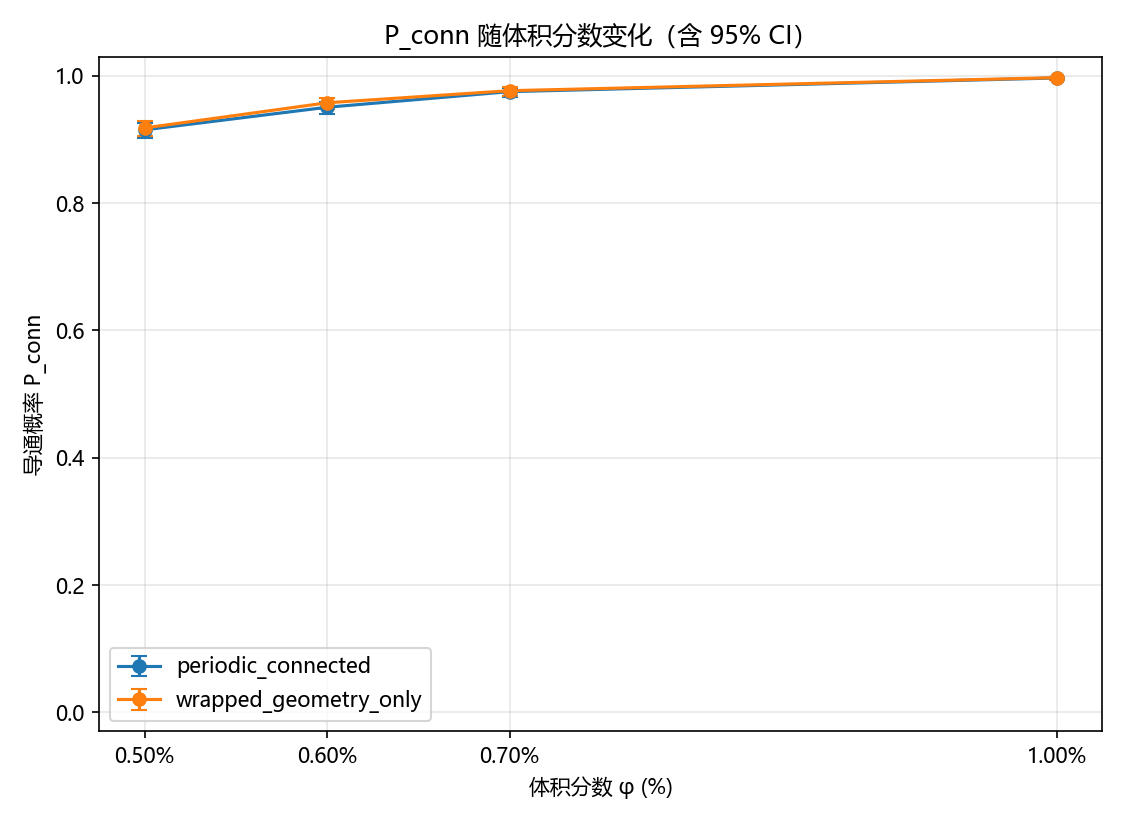
\includegraphics[width=0.72\textwidth]{version_log/2.0.0/conductive_microstructure/results/figures/problem2_p_conn.png}
    \caption{问题 2 中导通概率 $P_{\mathrm{conn}}$ 随体积分数 $\phi$ 的变化，两种边界模式下结果均随 $\phi$ 增大而单调上升。}
    \label{fig:q2_pconn}
\end{figure}

\begin{figure}[htbp]
    \centering
    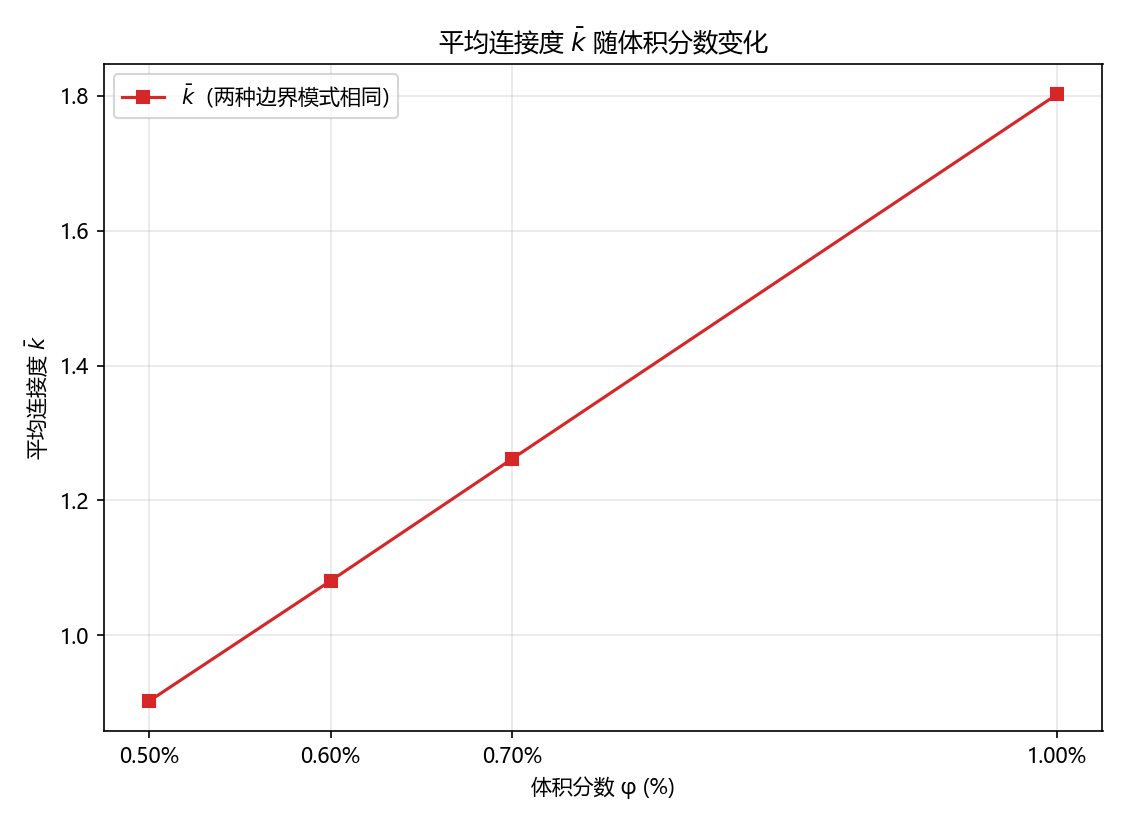
\includegraphics[width=0.72\textwidth]{version_log/2.0.0/conductive_microstructure/results/figures/problem2_kbar.png}
    \caption{问题 2 中概率云理论平均连接度 $\bar{k}$ 随体积分数 $\phi$ 的变化。随着填充率增加，单个节点的平均连接能力随之增强。}
    \label{fig:q2_kbar}
\end{figure}

\begin{figure}[htbp]
    \centering
    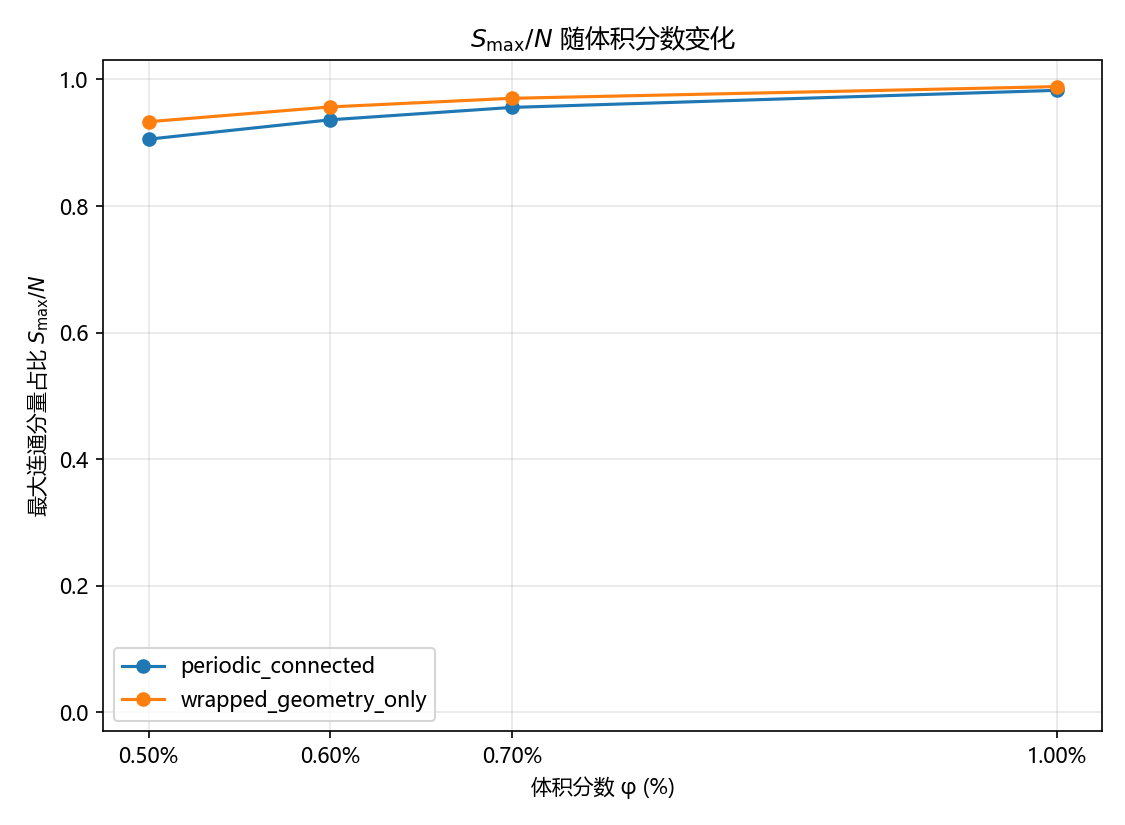
\includegraphics[width=0.72\textwidth]{version_log/2.0.0/conductive_microstructure/results/figures/problem2_smax_ratio.png}
    \caption{问题 2 中最大连通分量占比 $S_{\max}/N$ 随体积分数 $\phi$ 的变化。该指标反映了网络从分散小团簇向主导连通骨架演化的过程。}
    \label{fig:q2_smax}
\end{figure}

\begin{figure}[htbp]
    \centering
    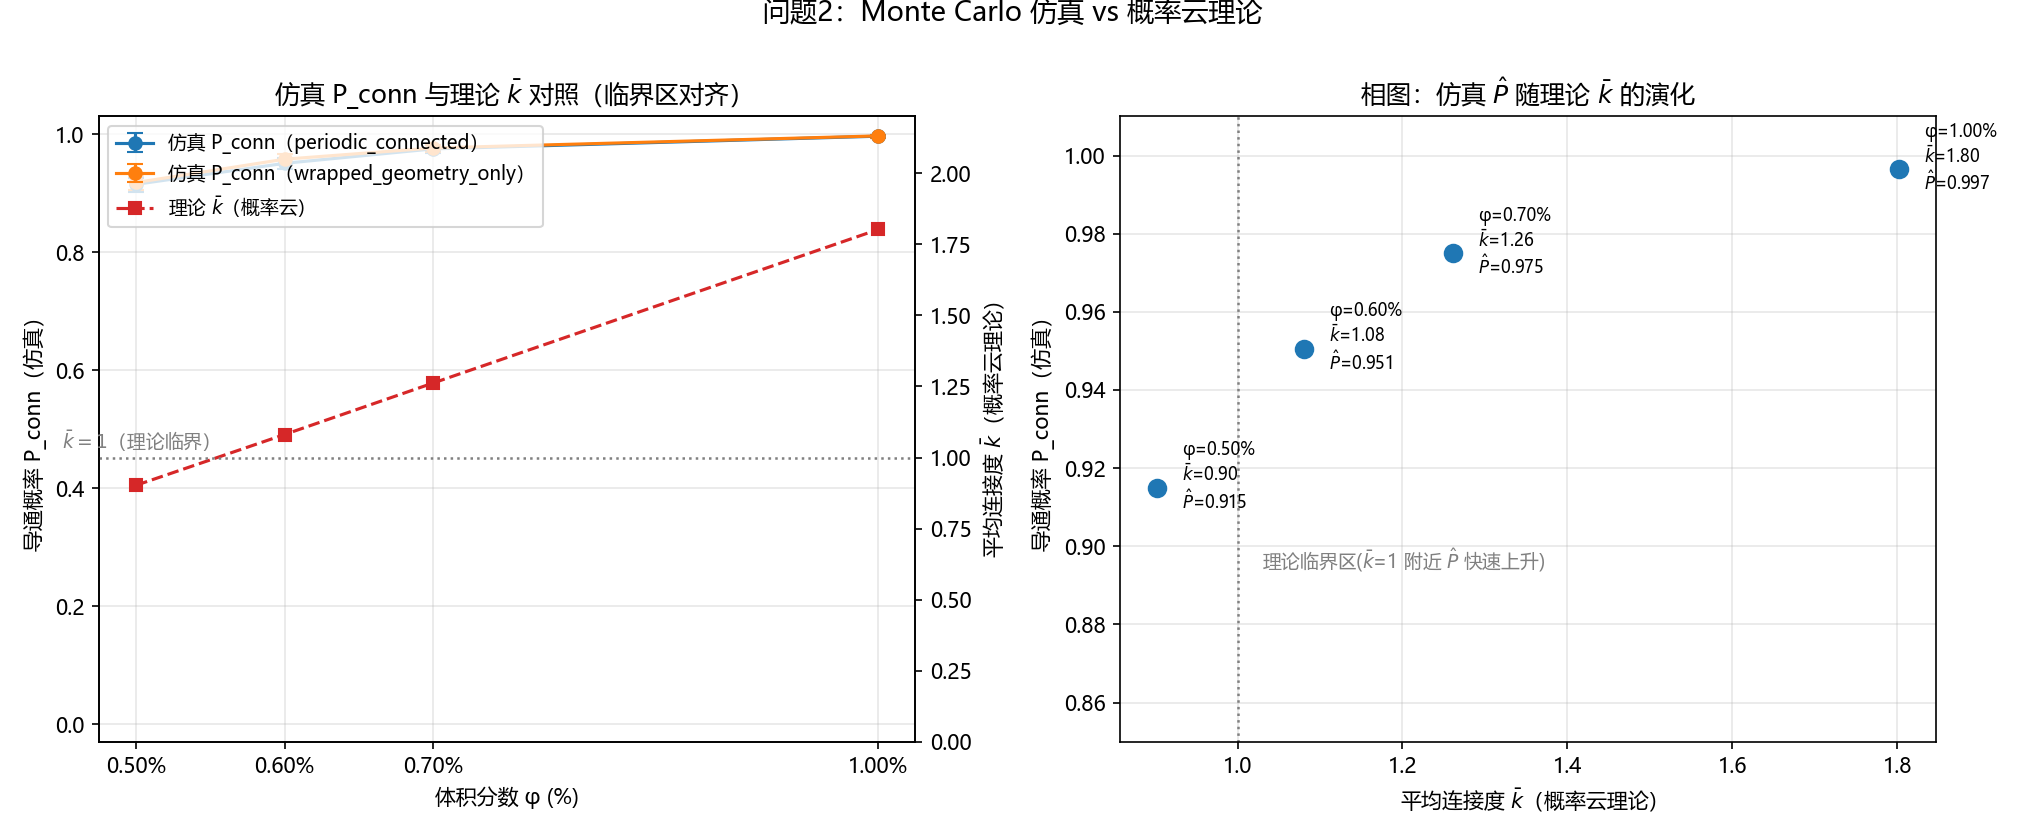
\includegraphics[width=0.92\textwidth]{version_log/2.0.0/conductive_microstructure/results/figures/problem2_theory_vs_simulation.png}
    \caption{问题 2 中 Monte Carlo 仿真与概率云理论的对照。左图展示导通概率与平均连接度随体积分数的变化，右图给出 $\hat{P}_{\mathrm{conn}}$ 与 $\bar{k}$ 的对应关系。}
    \label{fig:q2_theory_vs_sim}
\end{figure}

\section{问题 3：满足 \texorpdfstring{$P_{\mathrm{conn}}\ge 90\%$}{Pconn>=90\%} 的最低填充率}

\subsection{二分搜索与单侧置信判据}

问题 3 的目标是求满足
\[
P_{\mathrm{conn}}\ge 0.90
\]
时介质 A 的最低体积分数 $\phi_{\min}$。由于填充率越大，体系整体连边越多，贯通概率总体上单调不减，因此可在区间
\[
[\phi_{\mathrm{low}},\phi_{\mathrm{high}}]=[0.20\%,0.70\%]
\]
上采用二分搜索。

为了避免仅凭点估计作出过于乐观的判断，本文使用 Wilson 单侧 $95\%$ 置信下界
\[
p_{\mathrm{lower},95\%}\ge 0.90
\]
作为“达标”的统计判据。若直接使用 $\hat{P}_{\mathrm{conn}}\ge 0.90$，则在真实概率恰处于临界附近时，容易因抽样波动而误判；而采用单侧置信下界可以保证结论更稳健。

\subsection{理论临界值}

由问题 2 已得
\[
V_{AA}=2.5493\times 10^9\,\mathrm{nm}^3.
\]
令平均连接度满足
\[
\bar{k}=1,
\]
即可得到理论临界填充率
\[
\phi_{\mathrm{theory}}=\frac{V_A}{V_{AA}}\approx 0.005546=0.5546\%.
\]
这并不是“$90\%$ 导通”的精确解析公式，而是一个用于描述渗流临界位置的理论参考值。

\subsection{问题 3 结果}

在二分中点使用 $1000$ 次试验判定，收敛后对候选点使用 $4000$ 次试验复核，得到表 \ref{tab:q3_result}。

\begin{table}[htbp]
    \centering
    \caption{问题 3 的最低填充率结果}
    \label{tab:q3_result}
    \begin{tabular}{cccccc}
        \hline
        边界模式 & $\phi_{\min}$ & $N_A$ & $\hat{P}_{\mathrm{conn}}$ & $p_{\mathrm{lower},95\%}$ & $\phi_{\mathrm{theory}}$ \\
        \hline
        周期连续 & 0.5125\% & 363 & 0.9155 & 0.9080 & 0.5546\% \\
        仅几何回绕 & 0.4969\% & 351 & 0.9075 & 0.8997 & 0.5546\% \\
        \hline
    \end{tabular}
\end{table}

可以看到，两种模式下的最低填充率都落在 $0.50\%$ 附近，且略低于理论临界值 $0.5546\%$。这表明概率云理论给出的临界参考与真实仿真结果在量级和变化方向上是一致的。其偏低的原因在于：介质 A 长径比较大，链式连接能力较强，因此在有限尺寸盒体中，达到 $90\%$ 贯通概率时所需的体积分数可以略低于均值场意义下的 $\bar{k}=1$ 临界点。

需要如实说明的是，\texttt{wrapped\_geometry\_only} 模式下最终 $4000$ 次复核得到
\[
p_{\mathrm{lower},95\%}=0.8997,
\]
略低于 $0.90$。这说明该点位于统计临界附近，属于由有限样本波动带来的边界现象，而不是模型失效。相较于问题 2 的趋势验证，问题 3 进一步给出了概率云理论与实际临界填充率之间的定量对应关系。

\begin{figure}[htbp]
    \centering
    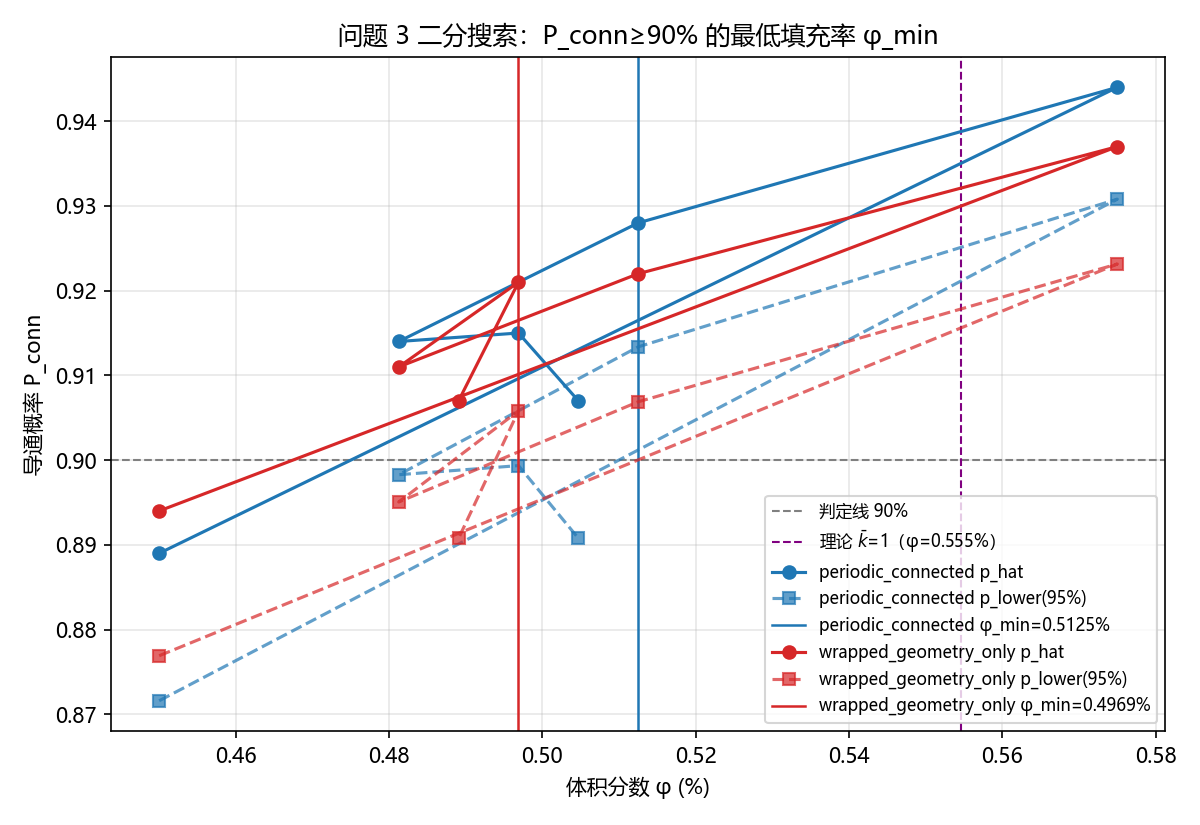
\includegraphics[width=0.72\textwidth]{version_log/2.0.0/conductive_microstructure/results/problem3/problem3_bisection.png}
    \caption{问题 3 中最低填充率的二分搜索过程示意图。图中展示了不同候选填充率下的判定结果及最终收敛区间。}
    \label{fig:q3_bisection}
\end{figure}

\section{问题 4：A/B 混合体系的最低成本组合}

\subsection{A/B 混合导通判据与成本函数}

在问题 4 中，除介质 A 外引入介质 B。其球心均匀分布在
\[
[-4800,4800]^3
\]
内，以保证球体完全落在盒内。混合体系的导通判据为：
\[
d_{AA}\le 61.8\,\mathrm{nm},\qquad
d_{AB}\le 231.8\,\mathrm{nm},\qquad
d_{BB}\le 401.8\,\mathrm{nm},
\]
且 B 球与电极平面导通的条件为球面到平面距离不超过 $\delta$，对应球心到电极面的距离阈值为 $201.8\,\mathrm{nm}$。

总成本函数写为
\[
C(N_A,N_B)=1.05\cdot N_A\frac{V_A}{10^9}+0.05\cdot N_B\frac{V_B}{10^9},
\]
其中
\[
V_B=\frac{4}{3}\pi R_B^3\approx 3.351\times 10^7\,\mathrm{nm}^3.
\]
目标是在
\[
P_{\mathrm{conn}}\ge 0.90
\]
的约束下，使成本最小。

\subsection{双介质概率云与连接矩阵}

在问题 2 的概率云思想基础上，定义混合体系中的三种等效连接体积：
\[
V_{AA},\qquad V_{AB},\qquad V_{BB}.
\]
其中 $V_{AA}$ 由问题 2 已得；$V_{BB}$ 可解析计算为半径 $401.8\,\mathrm{nm}$ 球体的体积；$V_{AB}$ 通过采样 A 的方向与 B 相对位置方向后数值积分得到。本文计算结果为
\[
V_{AA}=2.5493\times 10^9\,\mathrm{nm}^3,
\]
\[
V_{AB}=9.0877\times 10^8\,\mathrm{nm}^3,
\]
\[
V_{BB}=2.7172\times 10^8\,\mathrm{nm}^3.
\]
进一步构造连接矩阵
\[
M=
\begin{bmatrix}
\rho_A V_{AA} & \rho_B V_{AB}\\
\rho_A V_{AB} & \rho_B V_{BB}
\end{bmatrix},
\]
并以其最大特征值 $\lambda_{\max}$ 作为理论可行区的筛选指标。

\subsection{三级搜索策略}

问题 4 的求解采用“理论筛选 + Monte Carlo 边界搜索 + 成本优化确认”的三级流程：
\begin{enumerate}
    \item 在 $(N_A,N_B)$ 网格上扫描 $\lambda_{\max}$，得到理论可行区；
    \item 对每个 $N_A$ 网格点，在 $N_B\in[0,5000]$ 上用整数二分搜索满足 $p_{\mathrm{lower},95\%}\ge 0.90$ 的最小 $N_B$，得到可行边界；
    \item 沿边界计算成本，选取最小成本候选，并在其邻域用 $4000$ 次试验复核，最终确定最优解。
\end{enumerate}
之所以采用这种流程，是因为纯粹二维暴力扫描计算量极大，而理论可行区能够显著缩小需要精细仿真的范围。

\subsection{问题 4 结果与经济解释}

最终得到的最优解如表 \ref{tab:q4_result} 所示。

\begin{table}[htbp]
    \centering
    \caption{问题 4 的最低成本组合结果}
    \label{tab:q4_result}
    \begin{tabular}{cccccc}
        \hline
        边界模式 & $N_A^\ast$ & $N_B^\ast$ & 最低成本/元 & $\hat{P}_{\mathrm{conn}}$ & $p_{\mathrm{lower},95\%}$ \\
        \hline
        周期连续 & 360 & 0  & 5.3438 & 0.9147 & 0.9072 \\
        仅几何回绕 & 340 & 50 & 5.1307 & 0.9095 & 0.9018 \\
        \hline
    \end{tabular}
\end{table}

与此同时，理论层给出的 $\lambda_{\max}\ge 1$ 可行区为
\[
N_A\in[0,360],\qquad N_B\in[400,5000].
\]
与 Monte Carlo 实际边界相比，理论可行区明显偏宽松，但两者在趋势上是一致的：随着 $N_A$ 增大，所需的 $N_B$ 总体下降。这说明连接矩阵仍然成功刻画了局部连接能力的变化方向，只是有限尺寸下的实际贯通要求比均值场阈值更严格。

从工程解释看，最重要的结论不是“B 球越多越好”，而是：
\begin{quote}
    最低成本方案始终以介质 A 为主，介质 B 仅在临界区起到少量桥接补强作用。
\end{quote}
这是因为 B 球虽然单位体积成本较低，但单颗粒体积较大、点接触导电效率不如细长圆柱高；因此若试图依靠大量 B 球单独建立贯通路径，成本反而更高。只有当 A 已经接近形成主骨架时，加入少量 B 球才具有明显的边际收益。

\begin{figure}[htbp]
    \centering
    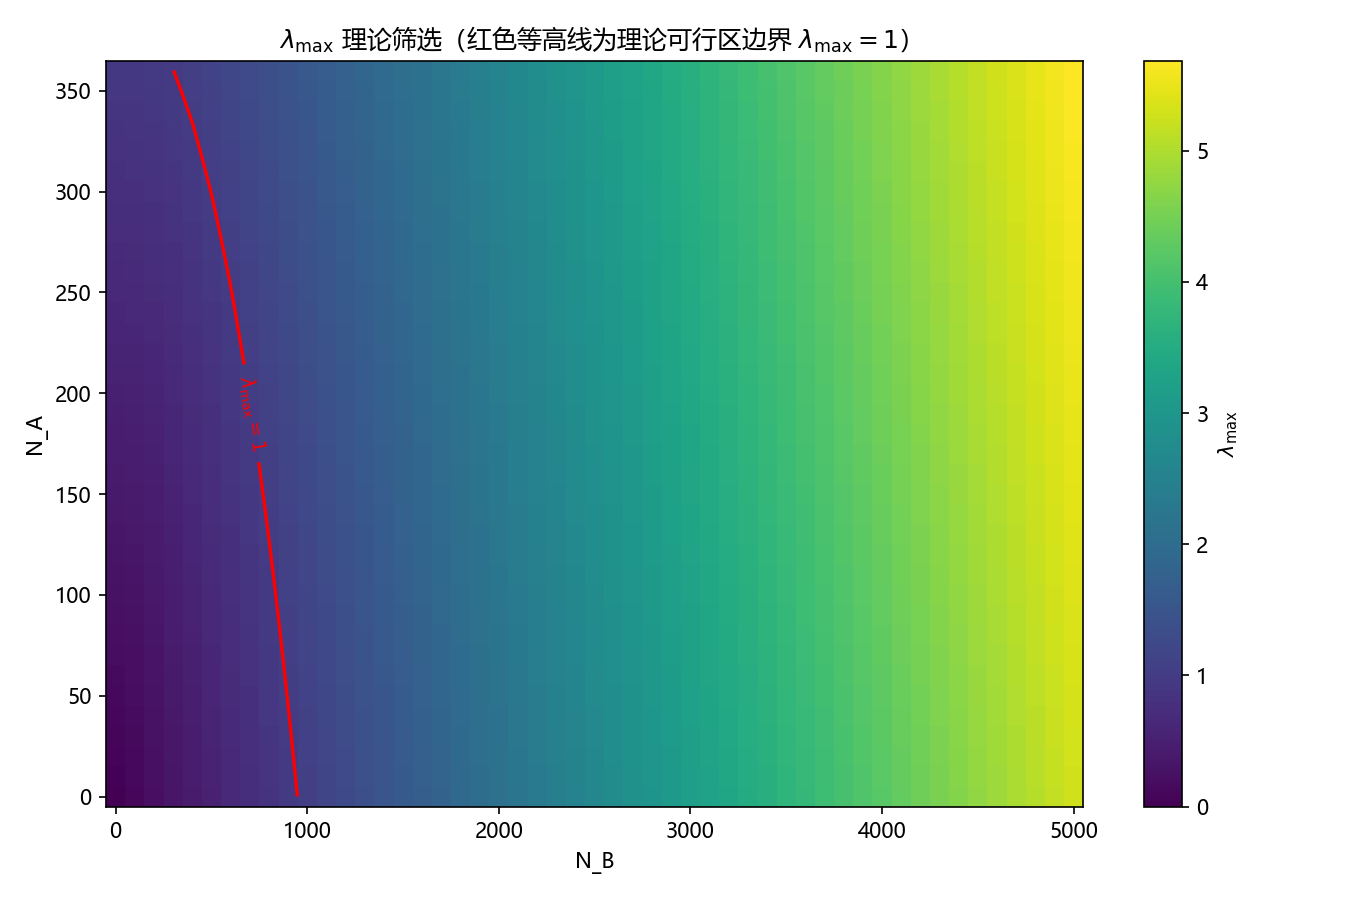
\includegraphics[width=0.78\textwidth]{version_log/2.0.0/conductive_microstructure/results/problem4/problem4_lambda_max_heatmap.png}
    \caption{问题 4 中 A/B 混合体系的 $\lambda_{\max}$ 理论热图。红色等高线对应 $\lambda_{\max}=1$，用于给出理论可行区。}
    \label{fig:q4_lambda}
\end{figure}

\begin{figure}[htbp]
    \centering
    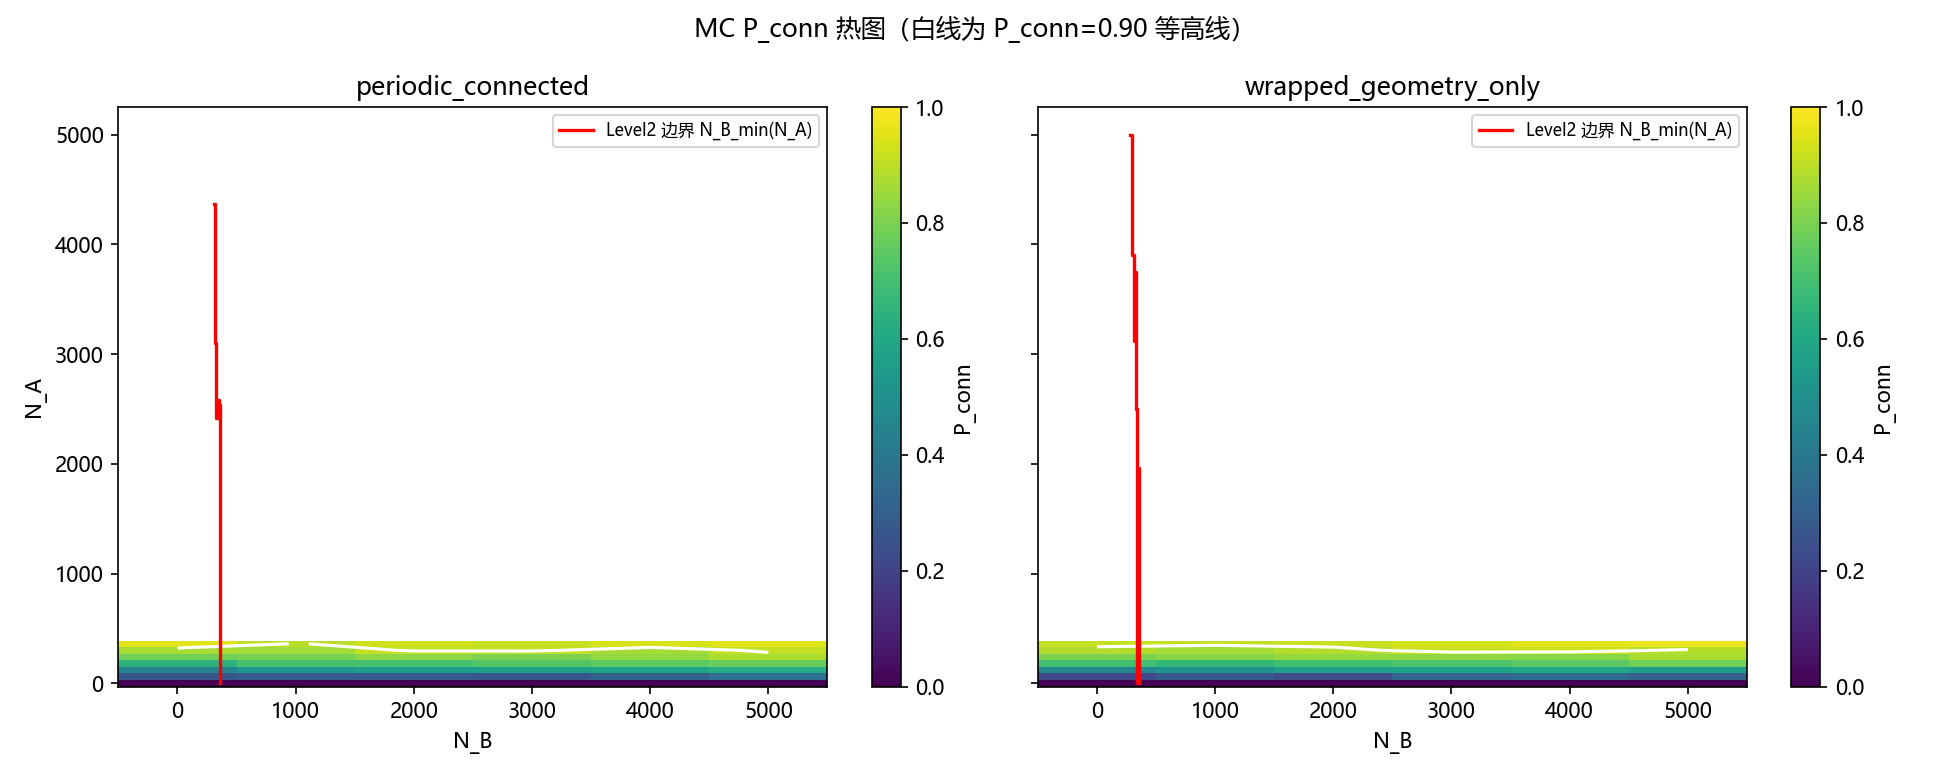
\includegraphics[width=0.92\textwidth]{version_log/2.0.0/conductive_microstructure/results/problem4/problem4_mc_pconn_heatmap.png}
    \caption{问题 4 中 A/B 混合体系的 Monte Carlo 导通概率热图。白色等高线为 $P_{\mathrm{conn}}=0.90$，红色阶梯线为二分搜索得到的可行边界。}
    \label{fig:q4_mc_heatmap}
\end{figure}

\begin{figure}[htbp]
    \centering
    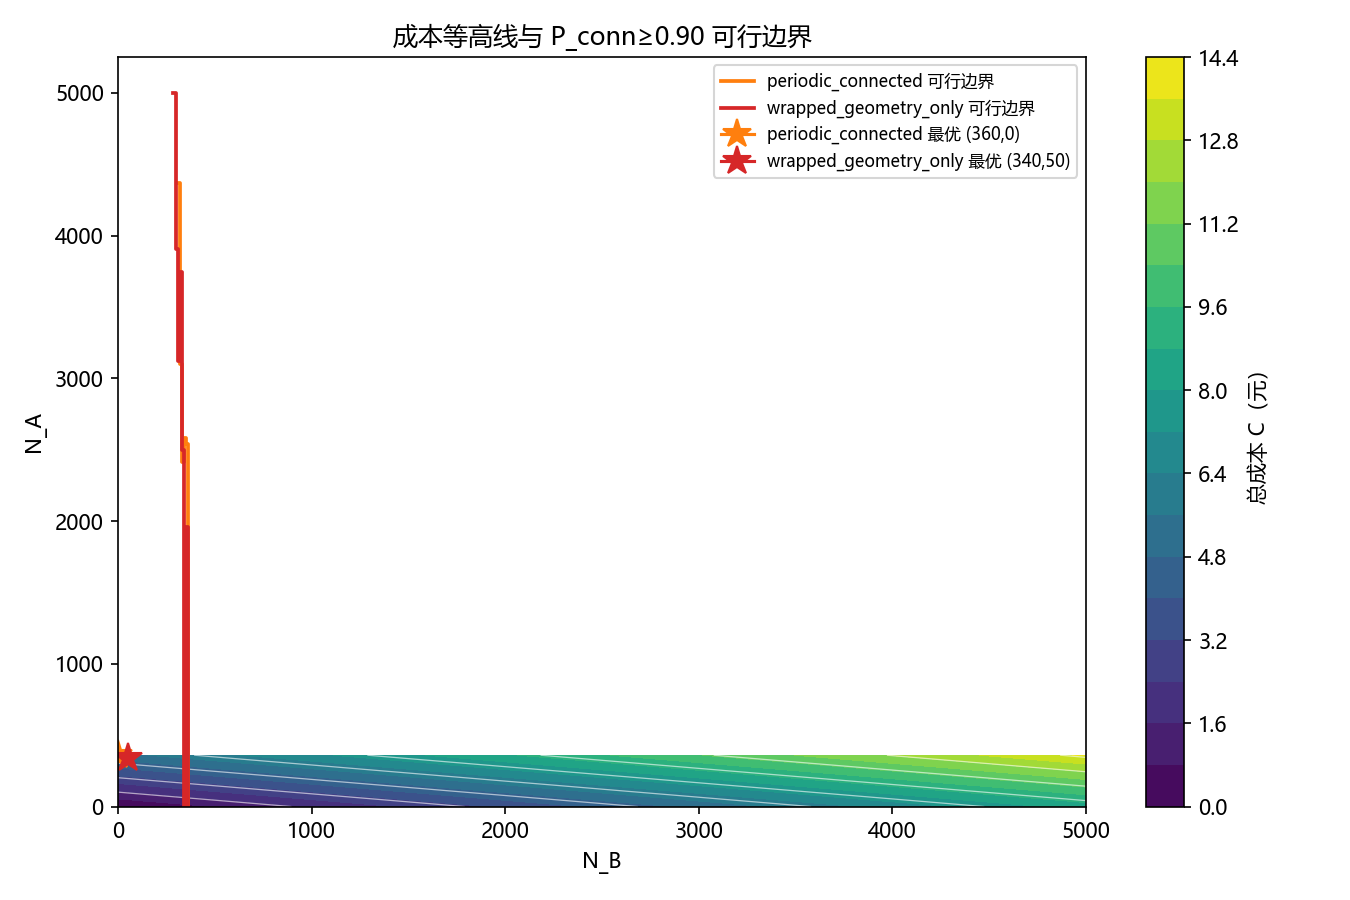
\includegraphics[width=0.78\textwidth]{version_log/2.0.0/conductive_microstructure/results/problem4/problem4_cost_boundary.png}
    \caption{问题 4 中成本等高线与可行边界。图中标出了满足 $P_{\mathrm{conn}}\ge 0.90$ 的最优组合位置。}
    \label{fig:q4_cost_boundary}
\end{figure}

\section{模型评价与结论}

\subsection{模型优点}

本文模型的主要优点体现在以下三个方面：
\begin{enumerate}
    \item 建立了统一的求解框架。问题 1 到问题 4 并非彼此割裂，而是围绕“局部连接 -- 宏观贯通 -- 优化决策”逐层展开；
    \item 理论与仿真互相支撑。概率云和连接矩阵负责解释渗流趋势与缩小搜索范围，Monte Carlo 负责给出有限尺寸盒体中的最终贯通概率；
    \item 结果具有较强可复现性。问题 3 的跨设备独立复现结果逐字节一致，说明当前随机种子派生和评估顺序设计可靠。
\end{enumerate}

\subsection{模型局限}

本文也存在以下局限：
\begin{enumerate}
    \item 圆柱之间的导通判据采用 capsule 近似，在端面附近存在微小几何误差；
    \item 概率云和连接矩阵基于各向同性随机分布的统计假设，未显式处理可能存在的取向偏置；
    \item 当前结论严格对应于题目给定的盒体尺度、几何参数和导通阈值，属于有限尺寸体系的工程结论。
\end{enumerate}

\subsection{全文结论}

综合问题 1 至问题 4 的结果，可以得到以下总体结论：
\begin{enumerate}
    \item 基于几何判距、边界处理和随机几何图的导通判定框架能够稳定刻画微构体中的导电贯通行为；
    \item 由局部连接概率云得到的等效连接体积与平均连接度，能够有效解释介质 A 体系中导通概率随填充率上升的规律；
    \item 满足 $P_{\mathrm{conn}}\ge 0.90$ 时，介质 A 的最低填充率约为 $0.50\%$，与理论临界值 $0.5546\%$ 同量级且方向一致，说明概率云理论已得到充分数值验证；
    \item 在 A/B 混合体系中，满足 $P_{\mathrm{conn}}\ge 0.90$ 的最低成本方案并不是以 B 为主体，而是以 A 为主、B 为辅的混合策略。
\end{enumerate}

因此，本文建立的“几何导通判据 -- 概率云 -- 渗流解释 -- Monte Carlo 验证 -- 优化求解”方法链，对微构体填充导电介质问题具有较好的统一解释能力和求解能力。

\section*{图表与结果文件对应说明}

正文涉及的主要图表可与现有结果文件对应如下。

公共目录：\texttt{version\_log/2.0.0/conductive\_microstructure/results/}

具体文件清单：
\begin{itemize}
    \small
    \item 问题 2 概率云图：\texttt{figures/problem2\_q\_aa.png}
    \item 问题 2 概率云积分核图：\texttt{figures/problem2\_4pir2q.png}
    \item 问题 2 导通概率图：\texttt{figures/problem2\_p\_conn.png}
    \item 问题 2 平均连接度图：\texttt{figures/problem2\_kbar.png}
    \item 问题 2 最大连通分量占比图：\texttt{figures/problem2\_smax\_ratio.png}
    \item 问题 2 理论--仿真对照图：\texttt{figures/problem2\_theory\_vs\_simulation.png}
    \item 问题 3 二分结果图：\texttt{problem3/problem3\_bisection.png}
    \item 问题 4 理论热图：\texttt{problem4/problem4\_lambda\_max\_heatmap.png}
    \item 问题 4 Monte Carlo 热图：\texttt{problem4/problem4\_mc\_pconn\_heatmap.png}
    \item 问题 4 成本边界图：\texttt{problem4/problem4\_cost\_boundary.png}
\end{itemize}

\section*{参考文献}

\begin{thebibliography}{99}
    \bibitem{huashu2026} 2026 第七届“华数杯”大学生数学建模竞赛 A 题：微构体中填充导电介质的仿真优化.
    \bibitem{attachment} 竞赛附件：\texttt{附件.xlsx}.
    \bibitem{format} 2026 第七届华数杯数学建模竞赛论文格式规范与提交说明.
\end{thebibliography}
